
\chapter{Методы моделирования ондуляторного излучения от электронного сгустка с конечным эмиттансом} \label{chapt2}
При обсуждении методов моделирования рассматривается только ондуляторное излучение. Отчасти это мотивировано относительной простотой рассмотрения ондуляторного излучения, по сравнению, например, с вигглерным \cite{geloni_brightness_2014}. С другой стороны, при рассмотрении источников четвёртного поколения, излучение из ондуляторов обладает высокой степенью поперечной когерентности, что и представляет интерес в рамках данной работы. Тем не менее, формула~\ref{eq:E_bunch} применима и для вигглерного излучения, и для излучения из поворотных магнитов. Для расчёта конечного поля по формуле~\ref{eq:E_bunch} необходимо сгенерировать $N_e$ полей от каждого электрона и сложить их. Таким образом получится одна реализация поля, далее необходимо повторить операцию генерации поля для $N_b$ реализаций и усреднить модули квадратов полей по получившемуся статистическому ансамблю. Метод является крайне медленным, поэтому в случае продольно некогерентного источника подойдёт метод реализованный в коде SRW \cite{chubar_accurate_1998}, \cite{chubar_simulation_2006}. Он основан на сложение интенсивностей полей от каждого электрона, где отсутствует необходимость усреднять по статистическому ансамблю, что ускоряет процесс вычисления. Оба метода будут обсуждаться в настоящей главе. 

Альтернативный подход в моделировании частично когерентного излучения основывается на декомпозиции функции поперечной когерентности на Гаусс-Шелл моды (разложение по полиномам Эрмита) описываемый в работах \cite{singer_modelling_2011}, \cite{hua_application_2012}, \cite{khubbutdinov_coherence_2019}, \cite{noauthor_iucr_nodate}. Однако, как отмечают авторы в \cite{khubbutdinov_coherence_2019}, \cite{noauthor_iucr_nodate} и аналитически описывается в \cite{geloni_transverse_2008}, разложение по полиномам Эрмита не применимо в случае, когда источник имеет высокую степень когерентности. Так как функции, которые описывают поведение ондуляторного излучения и в дальней зоне, и на источнике, имеют не гауссову природу.

В текущей главе описывается новый алгоритм моделирования синхротронного излучения. Алгоритм основывается на прямом моделировании стохастических процессов при генерации синхротронного излучения, вызванных дробовым шумом в электронном сгустке, с последующим ограничением пространственных гармоник шума эффективными размерами излучения. По своей природе алгоритм имеет оценочный характер, именно поэтому в главе приведён сравнительный анализ результатов СЕРВАЛа с методом сложения амплитуд, на примере ряда оптических систем. СЕРВАЛ показал себя, как мощный инструмент для оценки когерентных свойств синхротронного излучения, точность которого мало уступает методу сложения амплитуд, но при этом метод имеет преимущество в быстродействии. 
\section{Расчёт ондуляторного излучения прямым моделированием методом Монте-Карло}
Формула~\ref{eq:E_bunch} используется напрямую при моделирования ондуляторного излучения, как продольно когерентного, так и некогерентного. Распределение поля $\bar{E}_{\bot}(z_0, \omega, \vec{\eta}, \vec{\l}, \vec{r}_{\bot})$ может быть получено и аналитически, и численно, взятием интеграла по траекториям электрона в ондуляторе. В случае численного подхода излучение может быть рассчитано на любой частоте из первых принципов. При аналитическом подходе выражение для излучения на резонансной частоте $\omega$ фундаментальной гармоники от одного электрона\footnote{более общая формула для поля с некоторой отстройкой поля $\Delta \omega$ может быть найдена, например, в~\cite{onuki_undulators_2003}} с некоторыми углом $\vec{\eta}_k$ и координатой $\vec{\l}_k$ на входе в идеальный планарный ондулятор может быть записано как: 
\begin{align}
	\bar{E}_{\bot}(z_0, \omega, \vec{\eta}_k, \vec{l}_k, \vec{\theta} \;) =
&	-\frac{\omega e A_{JJ} L_w}{2c^2z_0}\frac{K}{\gamma}\exp{\bigg[i \frac{\omega z_0}{2c} \bigg|\vec{\theta} - \vec{\l}/z_0\bigg|^2 \bigg]} \cr & \times \sinc \bigg[\frac{\omega L_s |\vec{\theta} - (\vec{\l}/z_0) - \vec{\eta}|^2}{4c}\bigg],
	\label{eq:single_electron_far_field}
\end{align}
где $\vec{\theta} = \vec{r}/z_0$, $e$ -- заряд электрона, $\gamma$ -- Лоренц-фактор, $K$ -- параметр ондуляторности, $k_w = 2 \pi / \lambda_w$, где $\lambda_w$ -- период ондулятора. $A_{JJ} = J_0(\zeta) - J_1(\zeta)$, $\zeta = K^2/(4 + 2K^2)$ и $J_n$ -- функция Бесселя первого рода $n$ порядка. Формула \ref{eq:single_electron_far_field} даёт распределение амплитуды поля в дальней зоне. Определение дальней зоны для ондуляторного излучения обсуждается в~\cite{geloni_fourier_2007}. Чтобы получить точное выражение, это поле должно быть распространено обратно в центр ондулятора с помощью пропагатора свободного пространства~\cite{voelz_computational_2011},~\cite{schmidt_numerical_2010}, что даёт распределение поля в мнимом источнике излучения:
\begin{align}
	\bar{E}_{\bot}(0, \omega, \vec{\eta}, \vec{\l}, \vec{r}_{\bot}) =
	i \frac{e A_{JJ} \omega}{2 c^2}\frac{K}{\gamma} &\exp{\big[i \frac{\omega}{c} (\vec{r}_{\bot} - \vec{l})\big]}\cr & \times \bigg [\pi - 2\text{Si} \bigg( \cfrac{i \omega |\vec{r}_{\bot} - \vec{l}|^2}{L_w c}\bigg)\bigg], 
	\label{eq:single_electron_near_field_z=0}
\end{align}
после этого поле можно распространять на любое расстояние вдоль оптической оси $z$, что показано в~\cite{geloni_fourier_2007}. Таким образом, снова применяя пропагатор свободного пространства, получается:
\begin{align}
	\bar{E}_{\bot}(&z_0, \omega, \vec{\eta}_k, \vec{\l}_k, \vec{r}_{\bot}) =
		\frac{e A_{JJ} \omega}{2 c^2}\frac{K}{\gamma} \exp{\bigg[i \frac{\omega}{2 z_0 c} (|\vec{r}_{\bot} - \vec{l}|^2 - |\vec{r}_{\bot} - \vec{l} - z_0 \vec{\eta}|^2) \bigg]} \cr & \times	\bigg \{ \text{Ei} \bigg[ \cfrac{i \omega (\vec{r}_{\bot} - \vec{l} - z_0 \vec{\eta})^2}{2z_0c - L_w c}\bigg] - \text{Ei} \bigg[ \cfrac{i \omega (\vec{r}_{\bot} - \vec{l} - z_0 \vec{\eta})^2}{2z_0c + L_w c} \bigg] \bigg\}.
	\label{eq:single_electron_near_field}
\end{align}
Рассчитанное поле по формуле~\ref{eq:single_electron_near_field} может быть использовано для любого значения $z_0$, кроме точки $z_0 = L_w/2$ и $r_{\bot} = 0$, см.~\cite{geloni_fourier_2007}, это выражение действительно как для дальней зоны, так и для ближней. Обе формулы \ref{eq:single_electron_far_field} и \ref{eq:single_electron_near_field} получены аналитически, взятием интеграла по траектории электрона в идеальном синусоидальном магнитном поле, при этом расчёт поля по формуле~\ref{eq:single_electron_near_field} значительно более трудоёмкий, чем по формуле~\ref{eq:single_electron_far_field}\footnote{Необходимо дважды численно взять интеграл $\text{Ei}(\cdot)$}. При использовании численных методик для взятия интеграла по траекториям в случае немодельных магнитных полей можно рассчитывать поля для любой частоты излучения. В итоге, рассчитанные поля $\bar{E}_{\bot}(z_0, \omega, \vec{\eta}_k, \vec{\l}_k, \vec{r}_{\bot})$ имеют практическую ценность при вычислении излучения от всего электронного сгустка по формуле~\ref{eq:E_bunch}. Для простоты, в дальнейшем все расчёты ондуляторного излучения проведены для резонансной частоты фундаментальной гармоники.
 
\subsection{Метод сложения амплитуд}
После расчёта суммарного поля c $N_e$ электронами по формуле~\ref{eq:E_bunch}, получившиеся монохроматическое поле по своей сути есть одна статистическая реализация. Это означает следующее: если измерить распределение интенсивности поля на детекторе от пролёта одного электронного сгустка, используя монохроматор, который позволит разрешить один спектральный спайк излучения в $\omega$-пространстве, то на детекторе будет распределение, эквивалентное по своим свойствам представленному на Рис.~\ref{fig:spikes2}. 
\begin{figure}[H]
	\centering 	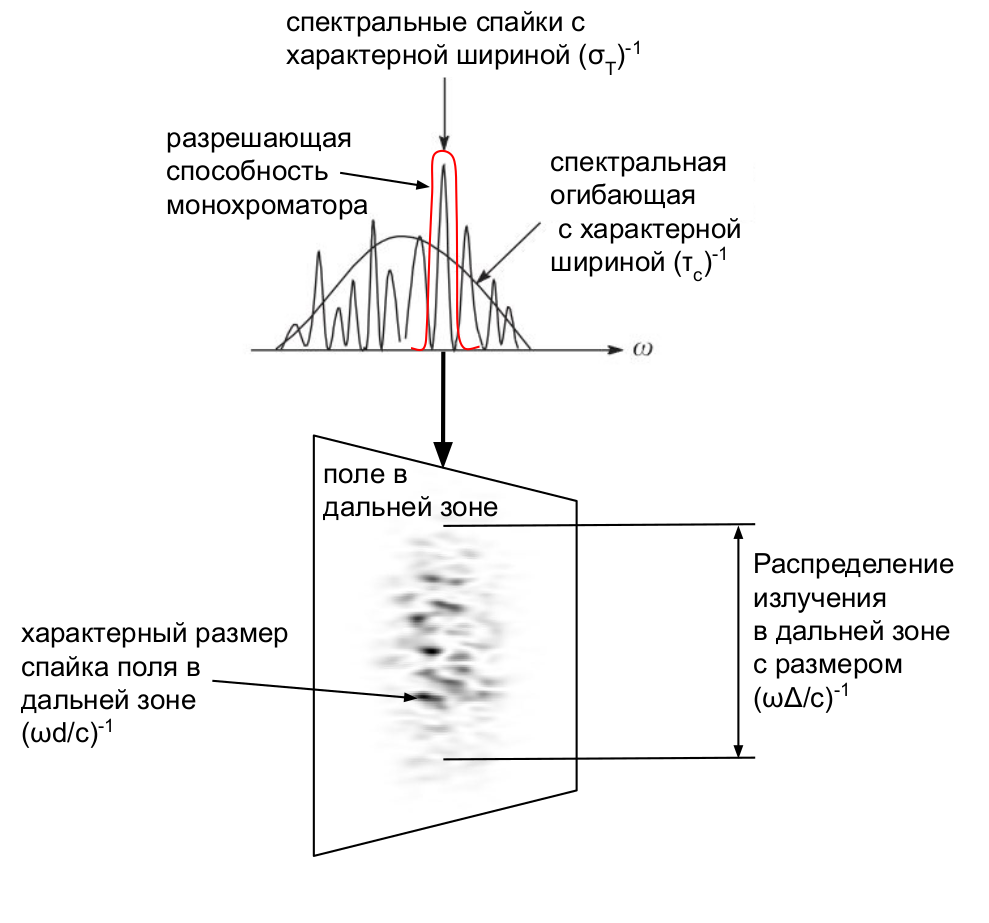
\includegraphics[width=0.7\linewidth]{spikes2.png}
	\caption{Спайковая структура излучения синхротронного излучения. Красной линией обозначена разрешающая способность монохроматора}
	\label{fig:spikes2}
\end{figure}
\noindent После усреднения по $N_b$ реализациям (с идеальным монохроматором\footnote{другими словами, монохроматором разрешается один спектральный спайк}), наблюдаемая интенсивность даётся выражением: 
\begin{align}
	I_{\omega} = \bigg \langle \bigg|\sum\limits_{k=1}^{N_e} \bar{E}(\vec{\eta}_k, \vec{\l}_k, z, \vec{r}, \omega) \exp{(i \omega t_k)}\bigg|^2 \bigg \rangle,
	\label{eq:I_MC} 
\end{align}
\noindent результирующая интенсивность будет сходиться к некоторой гладкой функции поперечных координат. В грубом приближении усреднённое угловое и пространственное распределение интенсивности излучения является свёрткой соответствующего распределения излучения от одного электрона с распределением всего электронного сгустка. Общая схема метода сложения амплитуд изображена на Рис.~\ref{fig:MC_scheme}. 
\begin{figure}[H] 
	\centering 	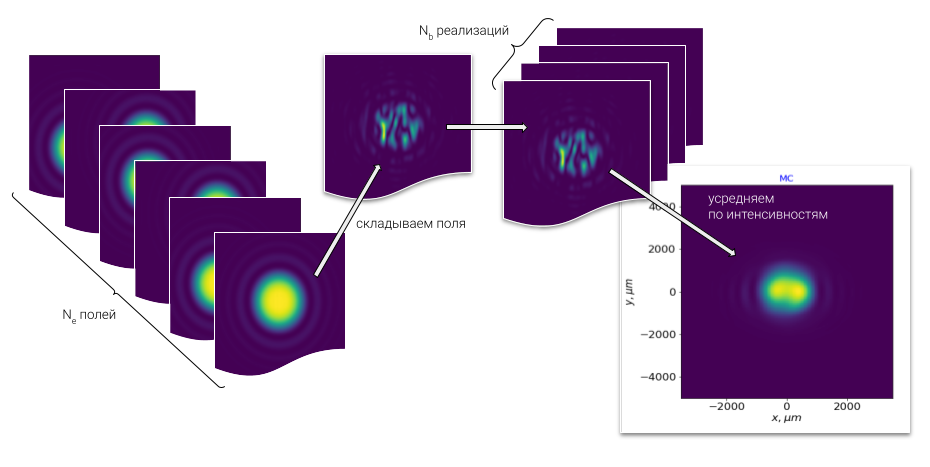
\includegraphics[width=0.99\linewidth]{MC_scheme.png}
	\caption{Схема работы метода сложения амплитуд}
	\label{fig:MC_scheme}
\end{figure}
Данный подход является наиболее прямым подходом в задаче моделирования частично когерентного излучения. Время расчёта, в таком случае, может быть оценено, как время затрачиваемое на расчёт одной реализации поля $N_e$ раз по формуле~\ref{eq:single_electron_far_field} или~\ref{eq:single_electron_near_field}, в последней, как уже упоминалось, необходимо дважды численно взять интеграл $\textup{Ei}(\cdot)$ и усреднить по $N_b$ реализациям поля $\bar{E}_{b}$. Итого, если за $\tau_{calc}$ взять время расчёта одного поля формуле~\ref{eq:single_electron_far_field} или~\ref{eq:single_electron_near_field}, то расчёт результирующего поля $\bar{E}_{b}$ в сумме займёт $T_{calc} = \tau_{calc} \cdot N_e \cdot N_b$.

\subsection{Метод сложения интенсивностей}
В случае полностью некогерентного излучения время расчёта можно сократить за счёт фазового фактора $\exp{(i \omega t_k)}$, который эффективно приводит к тому, что излучение отдельного электрона в электронном сгустке на каждом периоде ондулятора коррелирует только само с собой, \cite{geloni_transverse_2008}. Если расписать выражение~\ref{eq:I_MC}, получим: 
\begin{align}
	I_{\omega} = \sum\limits_{k=1}^{N_e} \bar{E}(\vec{\eta}_k, \vec{\l}_k, z, \vec{r}, \omega)\bar{E}^{*}(\vec{\eta}_k, \vec{\l}_k, z, \vec{r}, \omega) + \cr
	\bigg \langle \underset{k \neq n}{\sum\limits_{k=1}^{N_e} \sum\limits_{n=1}^{N_e}} \bar{E}(\vec{\eta}_k, \vec{\l}_k, z, \vec{r}, \omega)\bar{E}^{*}(\vec{\eta}_n, \vec{\l}_n, z, \vec{r}, \omega) & \exp{\big[i \omega (t_k - t_n)\big]}\bigg \rangle,
	\label{eq:I_SRW_with_explicit_sum} 
\end{align}
в котором после усреднения второе слагаемое будет равно нулю, так как $t_k$ и $t_n$ считаются независимыми случайными величинами. Таким образом формула~\ref{eq:I_MC} упрощается до 
\begin{align}
 	I_{\omega} = \sum\limits_{k=1}^{N_e} \bigg|\bar{E}(\vec{\eta}_k, \vec{\l}_k, z, \vec{r}, \omega)\bigg|^2,
 	\label{eq:I_SRW} 
\end{align}
а время расчёта уменьшается до $T_{calc} = \tau_{calc} \cdot N_e$. Этот метод, для условности, будет носить название метода сложения интенсивностей. Общая схема метода представлена на Рис.~\ref{fig:SRW_scheme}.
\begin{figure}[H] 
	\centering 	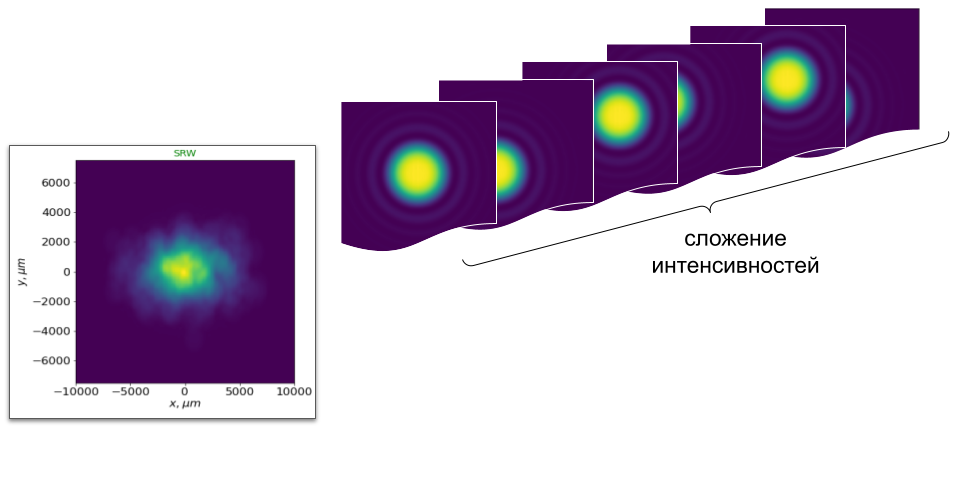
\includegraphics[width=0.99\linewidth]{SRW_scheme.png}
	\caption{Схема метода сложения интенсивностей}
	\label{fig:SRW_scheme}
\end{figure}
\noindent  Недостатком такого подхода можно считать потерю фазовой информации об излучении и, следовательно, невозможности расчёта функции поперечной когерентности первого порядка. Тем не менее, подход, основанный на формуле~\ref{eq:I_SRW}, даёт мощный метод расчёта наблюдаемых интенсивностей для частично когерентного излучения. Именно этот подход реализован в широко распространённом коде SRW.

В заключении к двум предыдущим разделам необходимо отметить: $N_b$ -- это физическая величина. Если разрешить монохроматором один спектральный спайк и набрать статистику, например, из десяти электронных сгустков, полученная интенсивность на детекторе будет соответствовать десяти реализациям поля. Иначе дело обстоит с числом макроэлектронов -- $N_e$. Для достоверного моделирования поперечной спайковой структуры синхротронного излучения необходимо взять число $N_e$ как минимум больше, чем характерное количество поперечных пространственных гармоник (спайков). Иначе, мелкие детали спайковой структуры не будут  разрешены монохроматором.
  
\section{Учёт влияния размера электронного сгустка на расходимость излучения при помощи прямых методов Монте-Карло}
При помощи метода сложения амплитуд можно получить поля, в которых видно влияние продольной когерентности\footnote{В смысле установленном в Главе~\ref{chapt1}.} излучения и размера электронного сгустка на расходимость излучения.
\subsection{Влияние размера электронного сгустка на расходимость излучения}
Первый эффект -- влияние размера электронного сгустка на расходимость излучения и, следовательно, на поперечный размер излучения в дальней зоне. Этот эффект обсуждается в работе~\cite{chubar_simulation_2006} разработчиком кода SRW применительно к когерентному синхротронному излучению (англ. coherent synchrotron radiation (CSR)). Под CSR подразумевает продольно когерентное излучение, реализуемое, когда длина электронного сгустка много меньше излучаемой длины волны. На примере CSR можно наблюдать следующий эффект: если электронный сгусток меньше или сравним с размером перетяжки излучения на источнике, наблюдается обычная расходимость излучения, определяемая свёрткой натуральной расходимости синхротронного излучения с расходимостью электронного сгустка.
\begin{figure}[H]
	\centering 	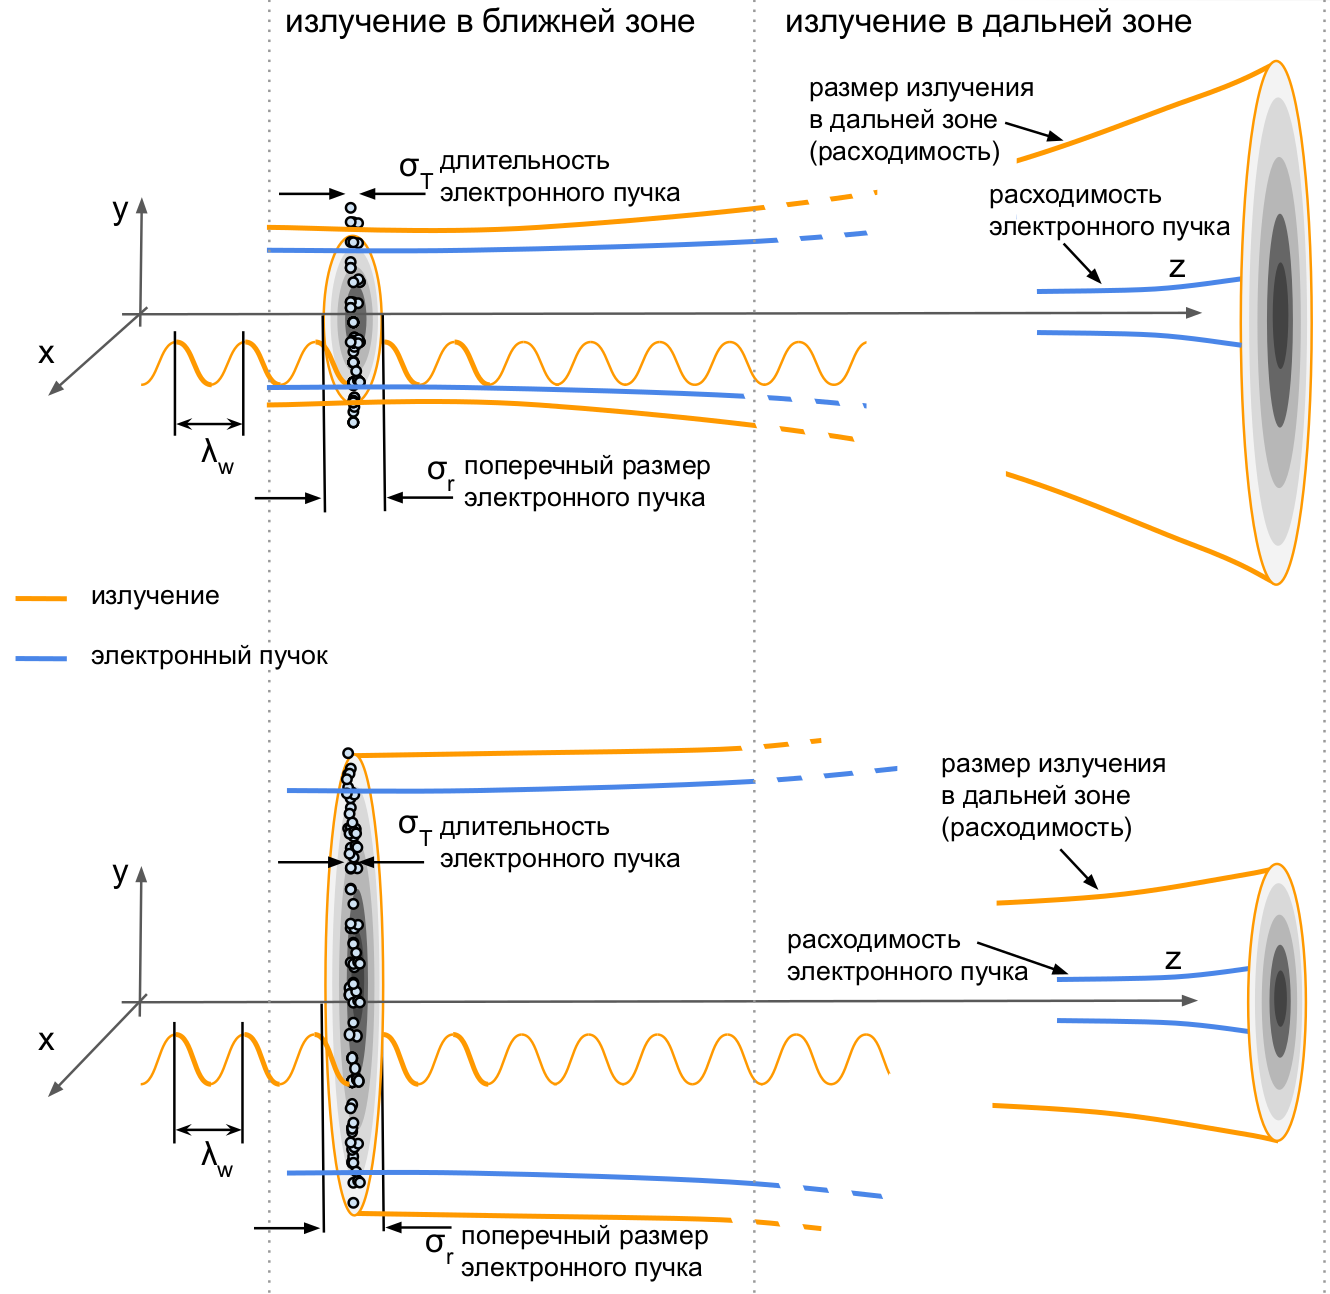
\includegraphics[width=0.99\linewidth]{diff_divergence_coh_scheme.png}
	\caption{Схема эффекта зависимости расходимости излучения от размера электронного сгустка. Рисунок разделён на две части: ближняя зона, источник излучения -- слева и дальняя зона -- справа. Жёлтой линией схематично изображён характерный поперечный размер излучения, синей линей характерный поперечный размер электронного сгустка, жёлтая волнистая линия символизирует длину волны излучения в сравнении с продольным размером электронного сгустка. Важно отметить, масштабы для обоих рисунков (верхнего и нижнего) одинаковы. Расходимости электронных сгустков (сверху и снизу) одинаковы.}
	\label{fig:diff_divergence_coh_scheme}
\end{figure}
Однако, при увеличении размера электронного сгустка, при той же расходимости, наблюдается эффект уменьшения расходимости излучения. Как отмечает автор в~\cite{chubar_simulation_2006}, этот эффект объясняется с точки зрения гауссовой оптики: при увеличении размера источника, угловой размер должен уменьшаться, формула~\ref{eq:photons_emittance}. На Рис~\ref{fig:diff_divergence_coh_scheme} изображена схема, описывающая этот эффект.

При расчёте ондуляторного излучения методом сложения амплитуд этот эффект выглядит следующим образом, \rr{Рис.~\ref{fig:diff_coh_incoh_rad}}.
\begin{figure}[H] 
	\centering 	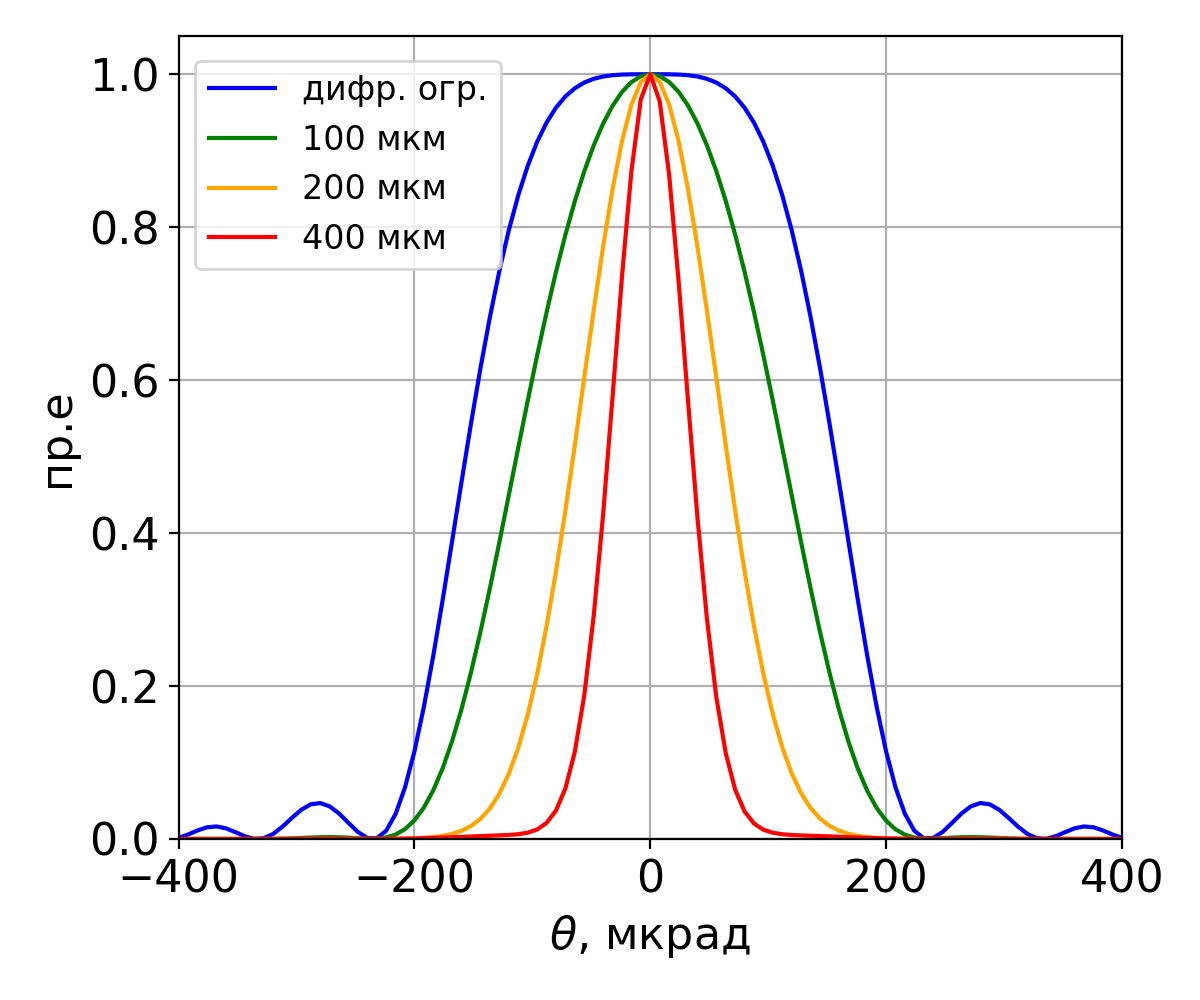
\includegraphics[width=0.5\linewidth]{diff_divergence_coh.png}
	\caption{Расходимость излучения от электронного сгустка с размерами, указанными в легенде. Расходимость электронного сгустка много меньше натуральной расходимости синхротронного излучения.}
	\label{fig:diff_coh_incoh_rad}
\end{figure}
Расчёт проводился для модельных параметров электронного сгустка: расходимость была взята много меньшей, чем натуральная расходимость ондуляторного излучения, размеры электронного сгустка указаны в легенде к Рис.~\ref{fig:diff_coh_incoh_rad}, резонансная энергия на $12,4$ эВ, ондулятор с $200$ периодами, длина периода ондулятора $18$ мм. Синяя линия на Рис.~\ref{fig:diff_coh_incoh_rad} отвечает случаю электронного сгустка с бесконечно малым эмиттансом.

\subsection{Различие расходимости излучения для случая продольно когерентного и некогерентного излучения}
В зависимости от длительности электронного сгустка результирующее поле $\bar{E}_{b}$ будет вести себя по-разному. В случае короткого электронного сгустка: $\omega \sigma_T \ll 1$, где $\sigma_T$ -- длительность электронного сгустка, излучение будет продольно когерентным, а в случай длинного электронного сгустка, а именно  $\omega \sigma_T \gg 1$, соответствует продольно некогерентному излучению. 

\begin{figure}[H] 
	\centering 	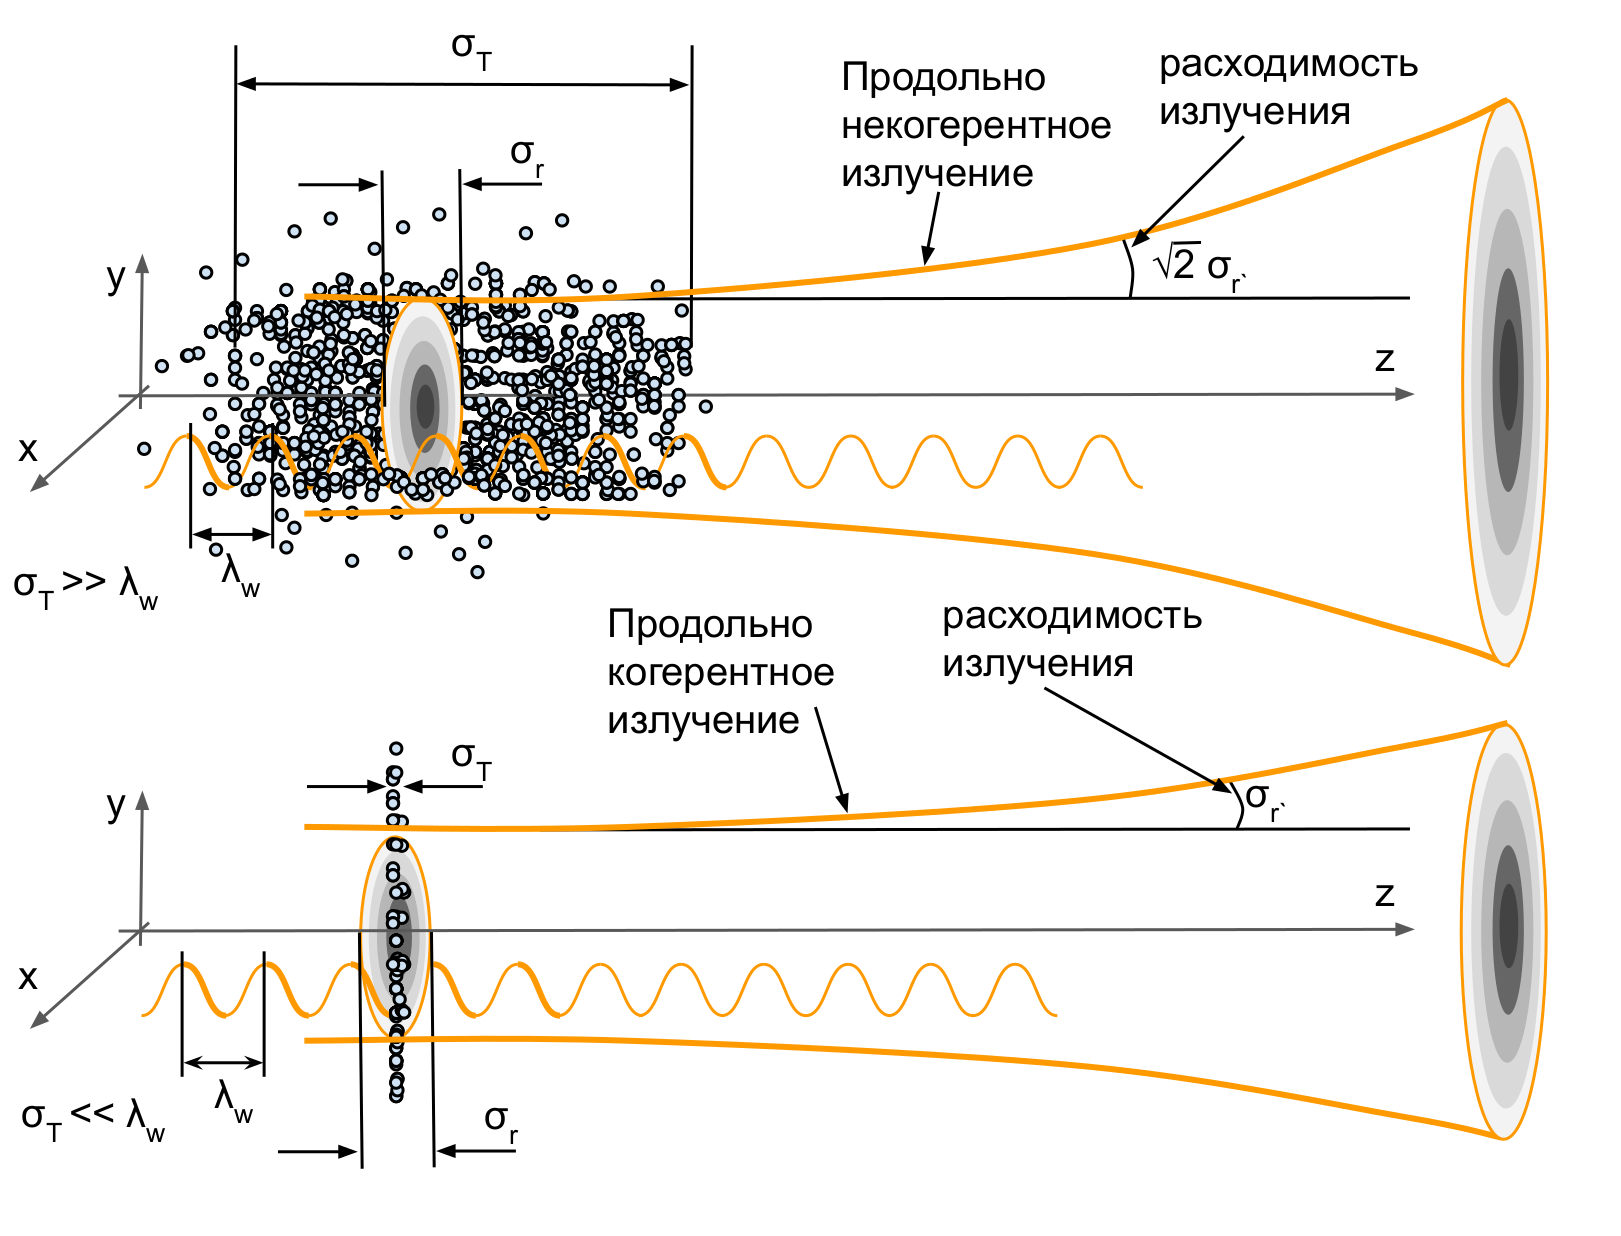
\includegraphics[width=0.99\linewidth]{coh_incoh_divergence.png}
	\caption{Схема эффекта зависимости расходимости излучения от продольной когерентности излучения. Жёлтой линией обозначен характерный поперечный размер излучения, жёлтой волнистой -- длина волны излучения с сравнение в продольным размером электронного сгустка. На рисунке обозначено, что в случае продольно некогерентного излучения расходимость в $\sqrt{2}$ раз больше, чем в случае продольно когерентного излучения.}
	\label{fig:coh_incoh_divergence}
\end{figure}
Расчёт проводился дли гипотетического случая электронного сгустка с поперечными размерами электронного сгустка много меньшими натуральных размеров излучения в перетяжке\footnote{Чтобы для продольно когерентного случая избежать эффекта, описанного в предыдущем разделе}, $\sigma_x' = 20$ мкрад, $\sigma_y' = 20$ мкрад на резонансной энергии $300$ эВ. Ондулятор с $200$ периодами, длина периода ондулятора $18$ мм. 

\begin{figure}[H] 
	\centering 	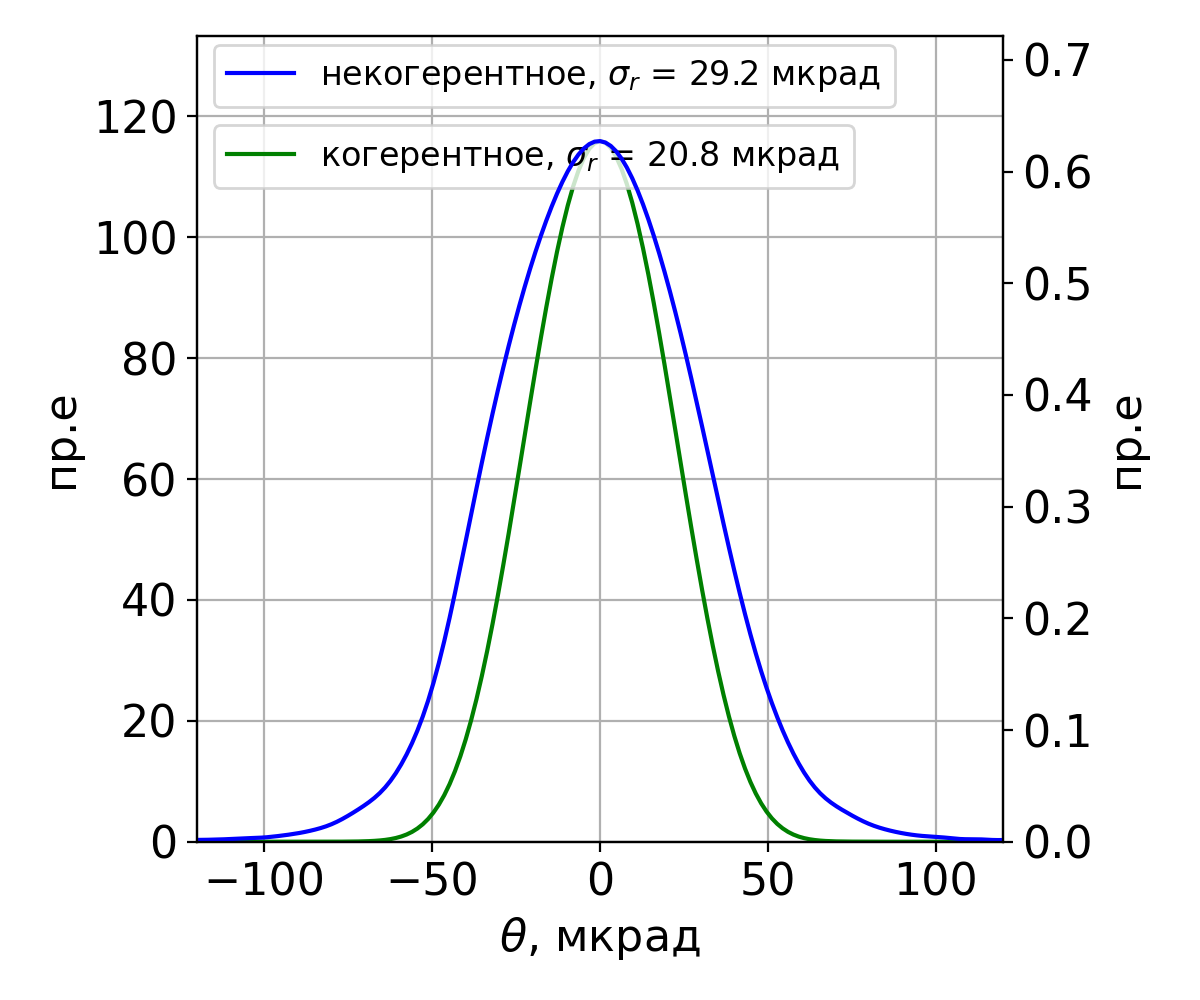
\includegraphics[width=0.5\linewidth]{diff_coh_incoh_rad.png}
	\caption{Расходимость излучения в случае продольно когерентного излучения (зелёная линия), и продольно некогерентного излучения (синяя линия).}
	\label{fig:diff_coh_incoh_rad}
\end{figure}
\noindent Этот эффект, по всей видимости, не обсуждался в литературе, однако, заслуживает дальнейшего исследования.
\section{Описание метода СЕРВАЛ}
Предлагаемый алгоритм основывается на моделировании стохастического характера ондуляторного синхротронного излучения комплексным гауссовым шумом с последующим его ограничением эффективным размером излучения на источнике. Алгоритм описывает продольное \textit{некогерентное} ондуляторное излучение. Для начала алгоритм будет представлен в общем виде, без уточнения, чем определяется вид гладких функций, задающих эффективный размер и расходимость излучения. 
\subsection{Алгоритм создания поля}
Алгоритм выполняется в три этапа: создание комплексного гауссового шума; его ограничение размерами излучения в перетяжке в $r$-пространстве; его ограничение расходимостью излучения в $k$-пространстве\footnote{Излучение от всего электронного сгустка.}. Полное описание алгоритма приведено ниже: 
\begin{enumerate}
\item \label{noise} Создание комлексного гауссового шума $Z = X + iY$ в $r\omega$-пространстве, где величины $X$ и $Y$ подчиняются нормальному распределению.
\begin{figure}[H] 
	\centering 	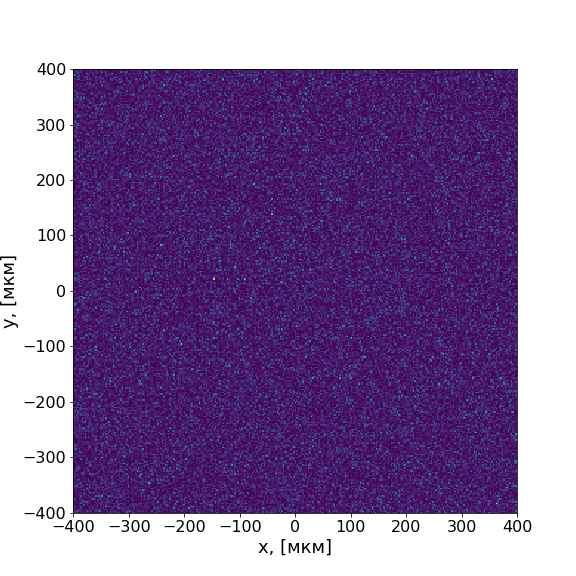
\includegraphics[width=0.45\linewidth]{1-X_noise.png}
	\caption{Интенсивность комплексного гауссового шума}
	\label{fig:1-noise}
\end{figure}
\item \label{beam_s} Ограничение шума эффективным размером электромагнитного излучения в источнике излучения в \textit{$r$}-пространстве.
\begin{figure}[H]
	\centering
	\begin{minipage}{0.45\textwidth}
		\centering
		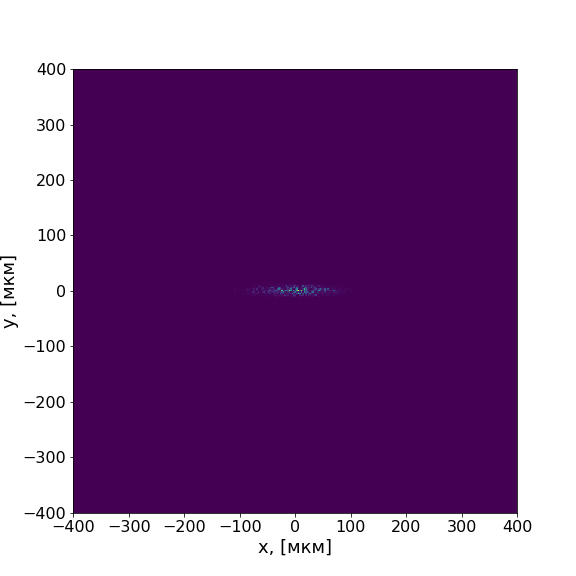
\includegraphics[width=1\linewidth]{2-X_e-beam-size.png}
		\caption{Размер излучение с наложенным шумом в $r$-пространстве}
		\label{fig:2-beam_size_k}
	\end{minipage}
	\begin{minipage}{0.45\textwidth}
		\centering
		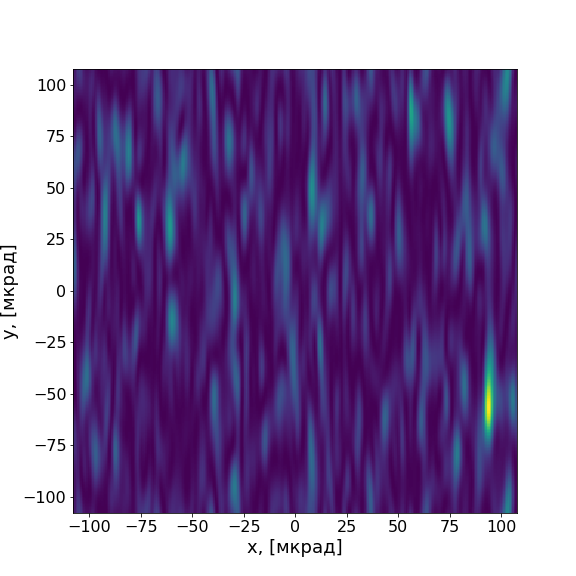
\includegraphics[width=1\linewidth]{2-X_e-beam-divergence.png}
		\caption{Размер излучение с наложенным шумом $k$-пространстве}
		\label{fig:2-beam_size_s}
	\end{minipage}\hfill
\end{figure}
\item \label{beam_k} Ограничение пространственных частот эффективной расходимостью излучения.
\begin{figure}[H]
	\centering
	\begin{minipage}{0.45\textwidth}
		\centering
		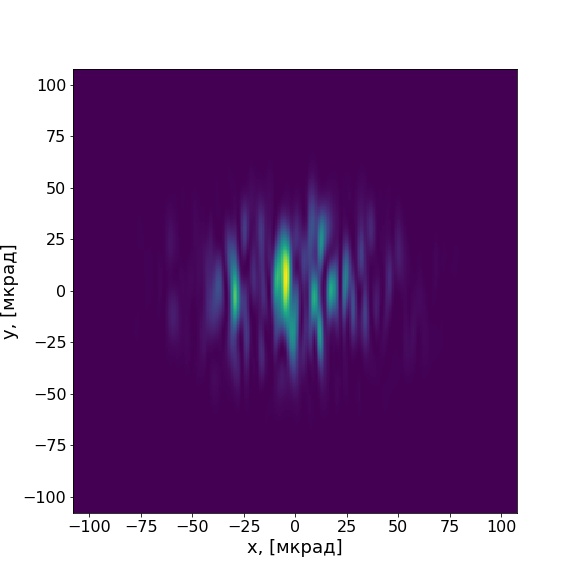
\includegraphics[width=1\linewidth]{3-X_radaition_divergence.png}
		\caption{Расходимость излучения в источнике}
		\label{fig:3-beam_s}
	\end{minipage}
	\begin{minipage}{0.45\textwidth}
		\centering
		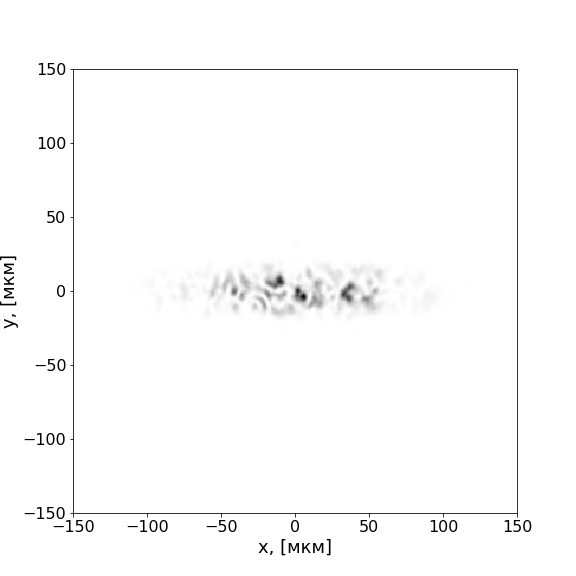
\includegraphics[width=1\linewidth]{3-X_radaition_size.png}
		\caption{Размер излучения в источнике}
		\label{fig:3-beam_k}
	\end{minipage}
\end{figure}
\end{enumerate}
\noindent Получившиеся распространение поля есть распределение поля в источнике излучения (центре ондулятора). Излучение монохроматично, т.е. продольно разрешён один спайк.

Быстродействие алгоритма можно оценить следующим образом: алгоритм генерирует $N_x \cdot N_y \cdot N_b$ случайных величин, подчиняющихся распределению $Z$, где $N_b$ -- количество реализаций поля, совершает одно преобразование Фурье (преобразование поля на Рис.~\ref{fig:2-beam_size_k} в поле на Рис.~\ref{fig:2-beam_size_s}) и два раза умножает поле на гладкие функции. Получившееся распределение, представленное на Рис.~\ref{fig:3-beam_k}, уже готово к распространению, так как пропагатор через свободное пространство работает именно в $k$-пространстве. 

Показательно сравнить быстродействие разобранных алгоритмов (Таблица~\ref{tab:speed}). При сравнении использовалась поперечная сетка $N_x \times N_y = 501 \times 501$, для расчёта поля в дальней зоне использовалась формула~\ref{eq:single_electron_far_field}. Сравнение производилось для разного количества макроэлектронов в методе сложения амплитуд.
\begin{table}[H]
	\caption{Быстродействие метода сложения амплитуд и СЕРВАЛа}
	\label{tab:speed}	
	\begin{tabular}{l|c|c|c}
	$N_e$ & МСА, сек/реализация &СЕРВАЛ, сек/реализация \\ 
	\hline
	100   & 2.8 & 0.020\\
	\hline 
	200   & 5.5 & 0.020 \\
	\hline 
	400   & 11  & 0.020 \\
	\end{tabular}
\end{table} 
\noindent Быстродействие метода сложения амплитуд и СЕРВАЛа сравнивается напрямую, так как в обоих методах есть необходимость усреднять по реализациям. Однако, для метода сложения интенсивностей нет понятия реализации поля, если только количество макроэлектронов. Для прямого сравнения СЕРВАЛА и метода сложения интенсивностей необходимо сравнивать быстроту генерации одного поля. Для той же плотности точек поперечной сетки, при равном числе реализаций и количестве макроэлектронов -- 400, расчёт поля СЕРВАЛом занял \textbf{8 сек}, методом сложения интенсивностей\footnote{Здесь снова стоит отметить, при использовании метода сложения интенсивностей теряется вся фазовая информация о поле, метод позволяет моделировать только наблюдаемые интенсивности полей.} \textbf{15 сек}. 
\subsection{Выбор подходящих распределений для ограничения пространственных гармоник шума}
До этого момента не обсуждался конкретный вид распределений, используемых для ограничения пространственных гармоник шума при генерации поля методом СЕРВАЛ. Вопрос выбора таких распределений сводится к нахождению пространственного и углового распределения поля в центре ондулятора. Поле в центре ондулятора может быть получено обратным распространением излучения из дальней зоны обратно в центр ондулятора при помощи пропагатора излучения в свободном пространстве. Однако, нахождение аналитического решения уравнения Максвелла в дальней зоне от целого электронного сгустка -- не тривиальная задача. Для оценки можно предположить, что распределение поля ондуляторного излучения от электронного сгустка с конечным эмиттансом, в целом, может быть представлено, как свёртка распределения поля ондуляторного излучения от одного электрона с распределением фазового пространства электронного сгустка~\cite{geloni_transverse_2008},~\cite{chubar_simulation_2006}.

Для СЕРВАЛа можно предложить, как минимум, три вида таких распределений. Для пространственного распределения источника в $r$-пространстве:
\begin{enumerate}[label=\Roman*.]
	\item \label{amplitude} ${A}_{b} (\vec{r}_{\bot}) = \big(\bar{E}_{\bot}(0, \vec{l}, \vec{\eta}, \vec{r}_{\bot}) \ast f_l(\vec{l})\big)(\vec{l})$ \\

	\item \label{intensity} ${A}_{b} (\vec{r}_{\bot}) = \sqrt{\big(\bar{E}^2_{\bot}(0,  \vec{l}, \vec{\eta}, \vec{r}_{\bot}) \ast f_l^2(\vec{l})\big)(\vec{l})}$ \\

	\item \label{e-beam} ${A}_{b} (\vec{r}_{\bot}) = f_l(\vec{l})$,
\end{enumerate}
и для расходимости источника в $k$-пространстве:
\begin{enumerate}[label=\Roman*.]
	\item \label{amplitude} $\hat{{A}}_{b} (\vec{\theta}_{\bot}) = \big(\hat{\bar{E}}_{\bot}(0,  \vec{l}, \vec{\eta}, \vec{\theta}_{\bot}) \ast \hat{f}_{\eta}(\vec{\eta})\big)(\vec{\eta})$\\
	
	\item \label{intensity} $\hat{{A}}_{b} (\vec{\theta}_{\bot}) = \sqrt{\big(\hat{\bar{E}}^2_{\bot}(0,  \vec{l}, \vec{\eta}, \vec{\theta}_{\bot}) \ast \hat{f_{\eta}^2}(\vec{\eta})\big)(\vec{\eta})}$\\
	
	\item \label{e-beam} $\hat{{A}}_{b} (\vec{\theta}_{\bot}) = \hat{f}_{\eta}(\vec{\eta})$,
\end{enumerate}
где ${A}_{b} (\vec{r})$ и $\hat{{A}}_{b} (\vec{\theta})$ гладкие функции поперечных координат в $r$- и $k$-пространствах, соответствующие шагам~\ref{beam_s} и~\ref{beam_k} в алгоритме,  $f(\vec{l}, \vec{\eta}) = f_l(\vec{l}) f_{\eta}(\vec{\eta})$ распределение фазового пространства электронного сгустка, и поле $\bar{E}_{\bot}(z=0, \vec{\l}, \vec{\eta}, \vec{r}_{\bot})$, $\hat{\bar{E}}_{\bot}(z=0 , \vec{\l}, \vec{\eta}, \vec{\theta}_{\bot})$ -- распределения поля в $r$ и $k$-пространствах, взятое в центре ондулятора, от электронного сгустка с бесконечно малым эмиттансом по формулам \ref{eq:single_electron_far_field} и \ref{eq:single_electron_near_field_z=0} или рассчитанные числено.

При выборе подходящих распределений было проведено сравнение с эталонным в этой работе методом сложения амплитуд. Для начала необходимо проверить распределение интенсивности поля на источнике. Для метода сложения амплитуд поле было рассчитано в дальней зоне и распространено назад в центр ондулятора. Результаты сравнения приведены на Рис.~\ref{fig:SERVAL_envelopes_comparison_source}-\ref{fig:SERVAL_envelopes_comparison_far_zone}. В работе использовались следующие параметры ондулятора, приведённые в Таблице~\ref{tab:undulator_parameters}.
\begin{table}[H]
	\caption{Параметры ондулятора}
	\label{tab:undulator_parameters}	
	\begin{tabular}{l|c|r}	
		$E_{ph},  [\textup{эВ}]/\lambda, [\textup{\AA}$]& $\lambda_w, [\textup{мм}]$ & периодов\\ 
		\hline	%0.65-1.35
		2167/5.72    &  18      & 200   
	\end{tabular}
\end{table}
\noindent Расчёты были проведены с использование параметров электронного сгустка ЦКП «СКИФ» для одного из прямых промежутков (Таблице~\ref{tab:SKIF parameters}).
\begin{table}[H]
	\caption{Параметры электронного сгустка}
	\label{tab:SKIF parameters}	
	\begin{tabular}{l|c|c|c|r}
		$E, \textup{[ГэВ]}$ & $\sigma_x, \textup{[мкм]}$ & $\sigma_y, \textup{[мкм]}$ & $\sigma_{x'}, \textup{[мкрад]}$ & $\sigma_{y'}, \textup{[мкрад]}$ \\ 
		\hline
		3          &38                          & 4.7                        & 25                          & 20 
	\end{tabular}
\end{table} 
\begin{figure}[H] 
	\centering 	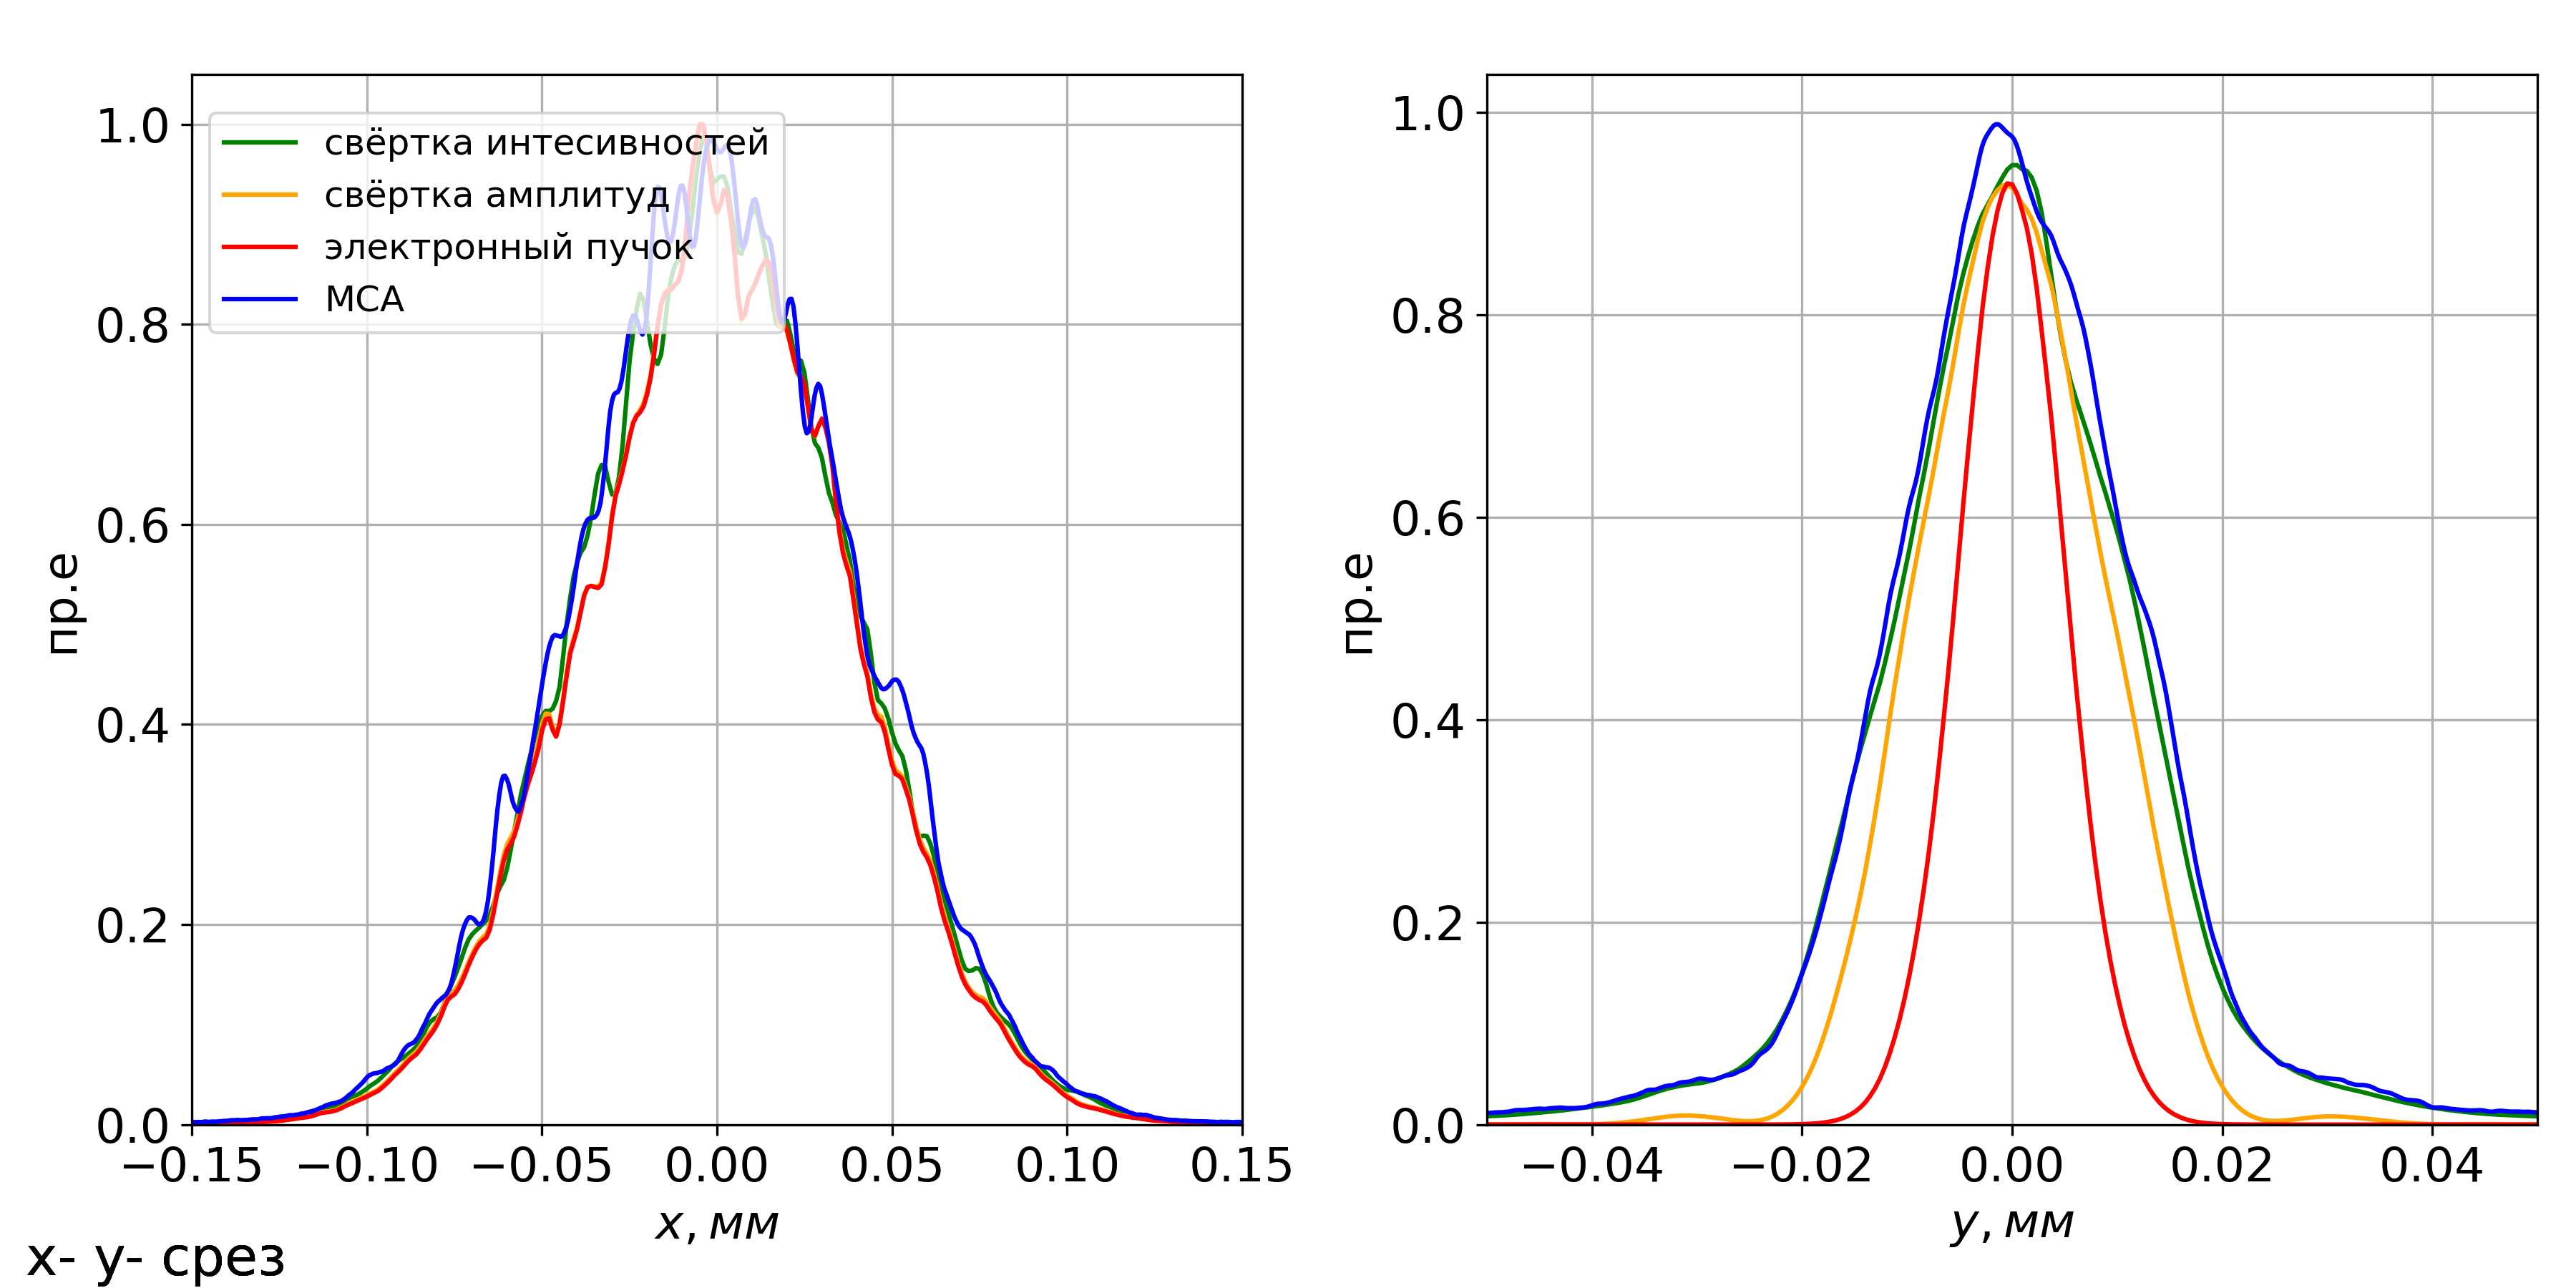
\includegraphics[width=0.99\linewidth]{SERVAL_envelopes_comparison_source.png}
	\caption{Распределение поля на источнике излучения для разных функций в сравнении с методом сложения амплитуд}
	\label{fig:SERVAL_envelopes_comparison_source}
\end{figure}
\noindent Видно, что оптимальные результаты достигаются при использовании свёртки~\ref{intensity} Однако, если размер электронного сгустка много больше или даже сравним с натуральным размером излучения в перетяжке, то можно использовать любые из представленных функций для $r$-пространства. Необходимо так же сравнить корреляционные функции получившихся полей~\ref{fig:SERVAL_envelopes_comparison_source} в дальней зоне на 25 м от ондулятора, используя формулу~\ref{eq:g1}.
\begin{figure}[H] 
	\centering 	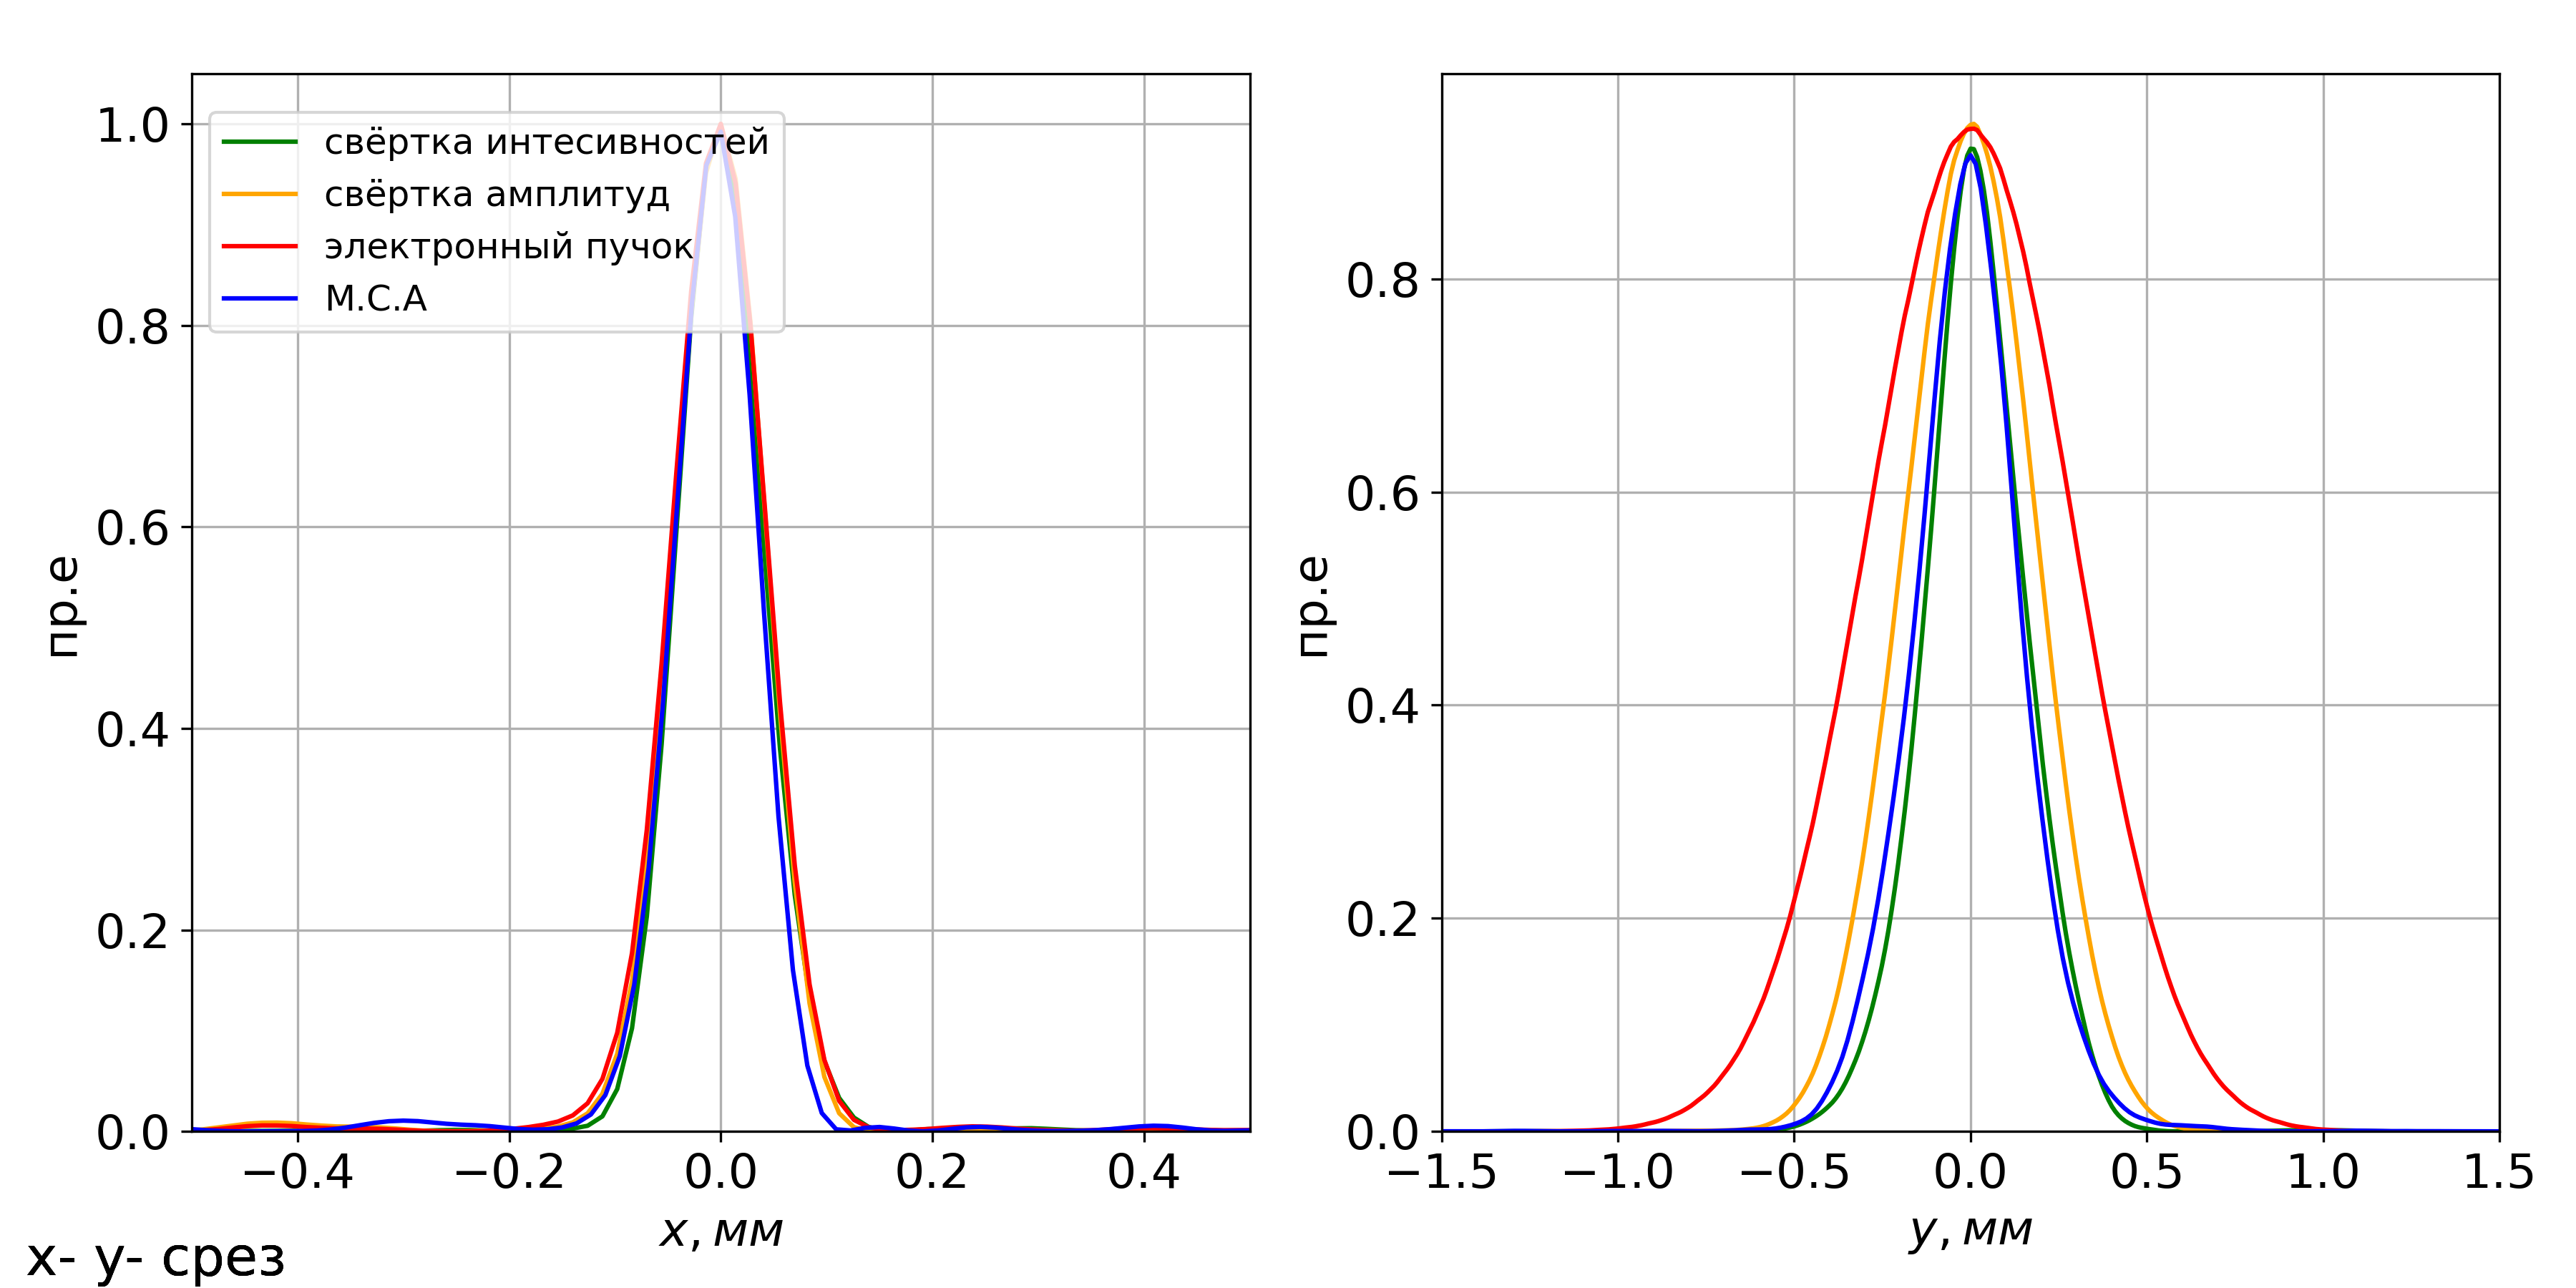
\includegraphics[width=0.99\linewidth]{SERVAL_corr_comparison.png}
	\caption{Функции поперечной когерентности на расстоянии $25$ м от источника}
	\label{fig:SERVAL_corr_comparison}
\end{figure}
\noindent Для распределения расходимости следует использовать свёртку интенсивностей.
\begin{figure}[H] 
	\centering 	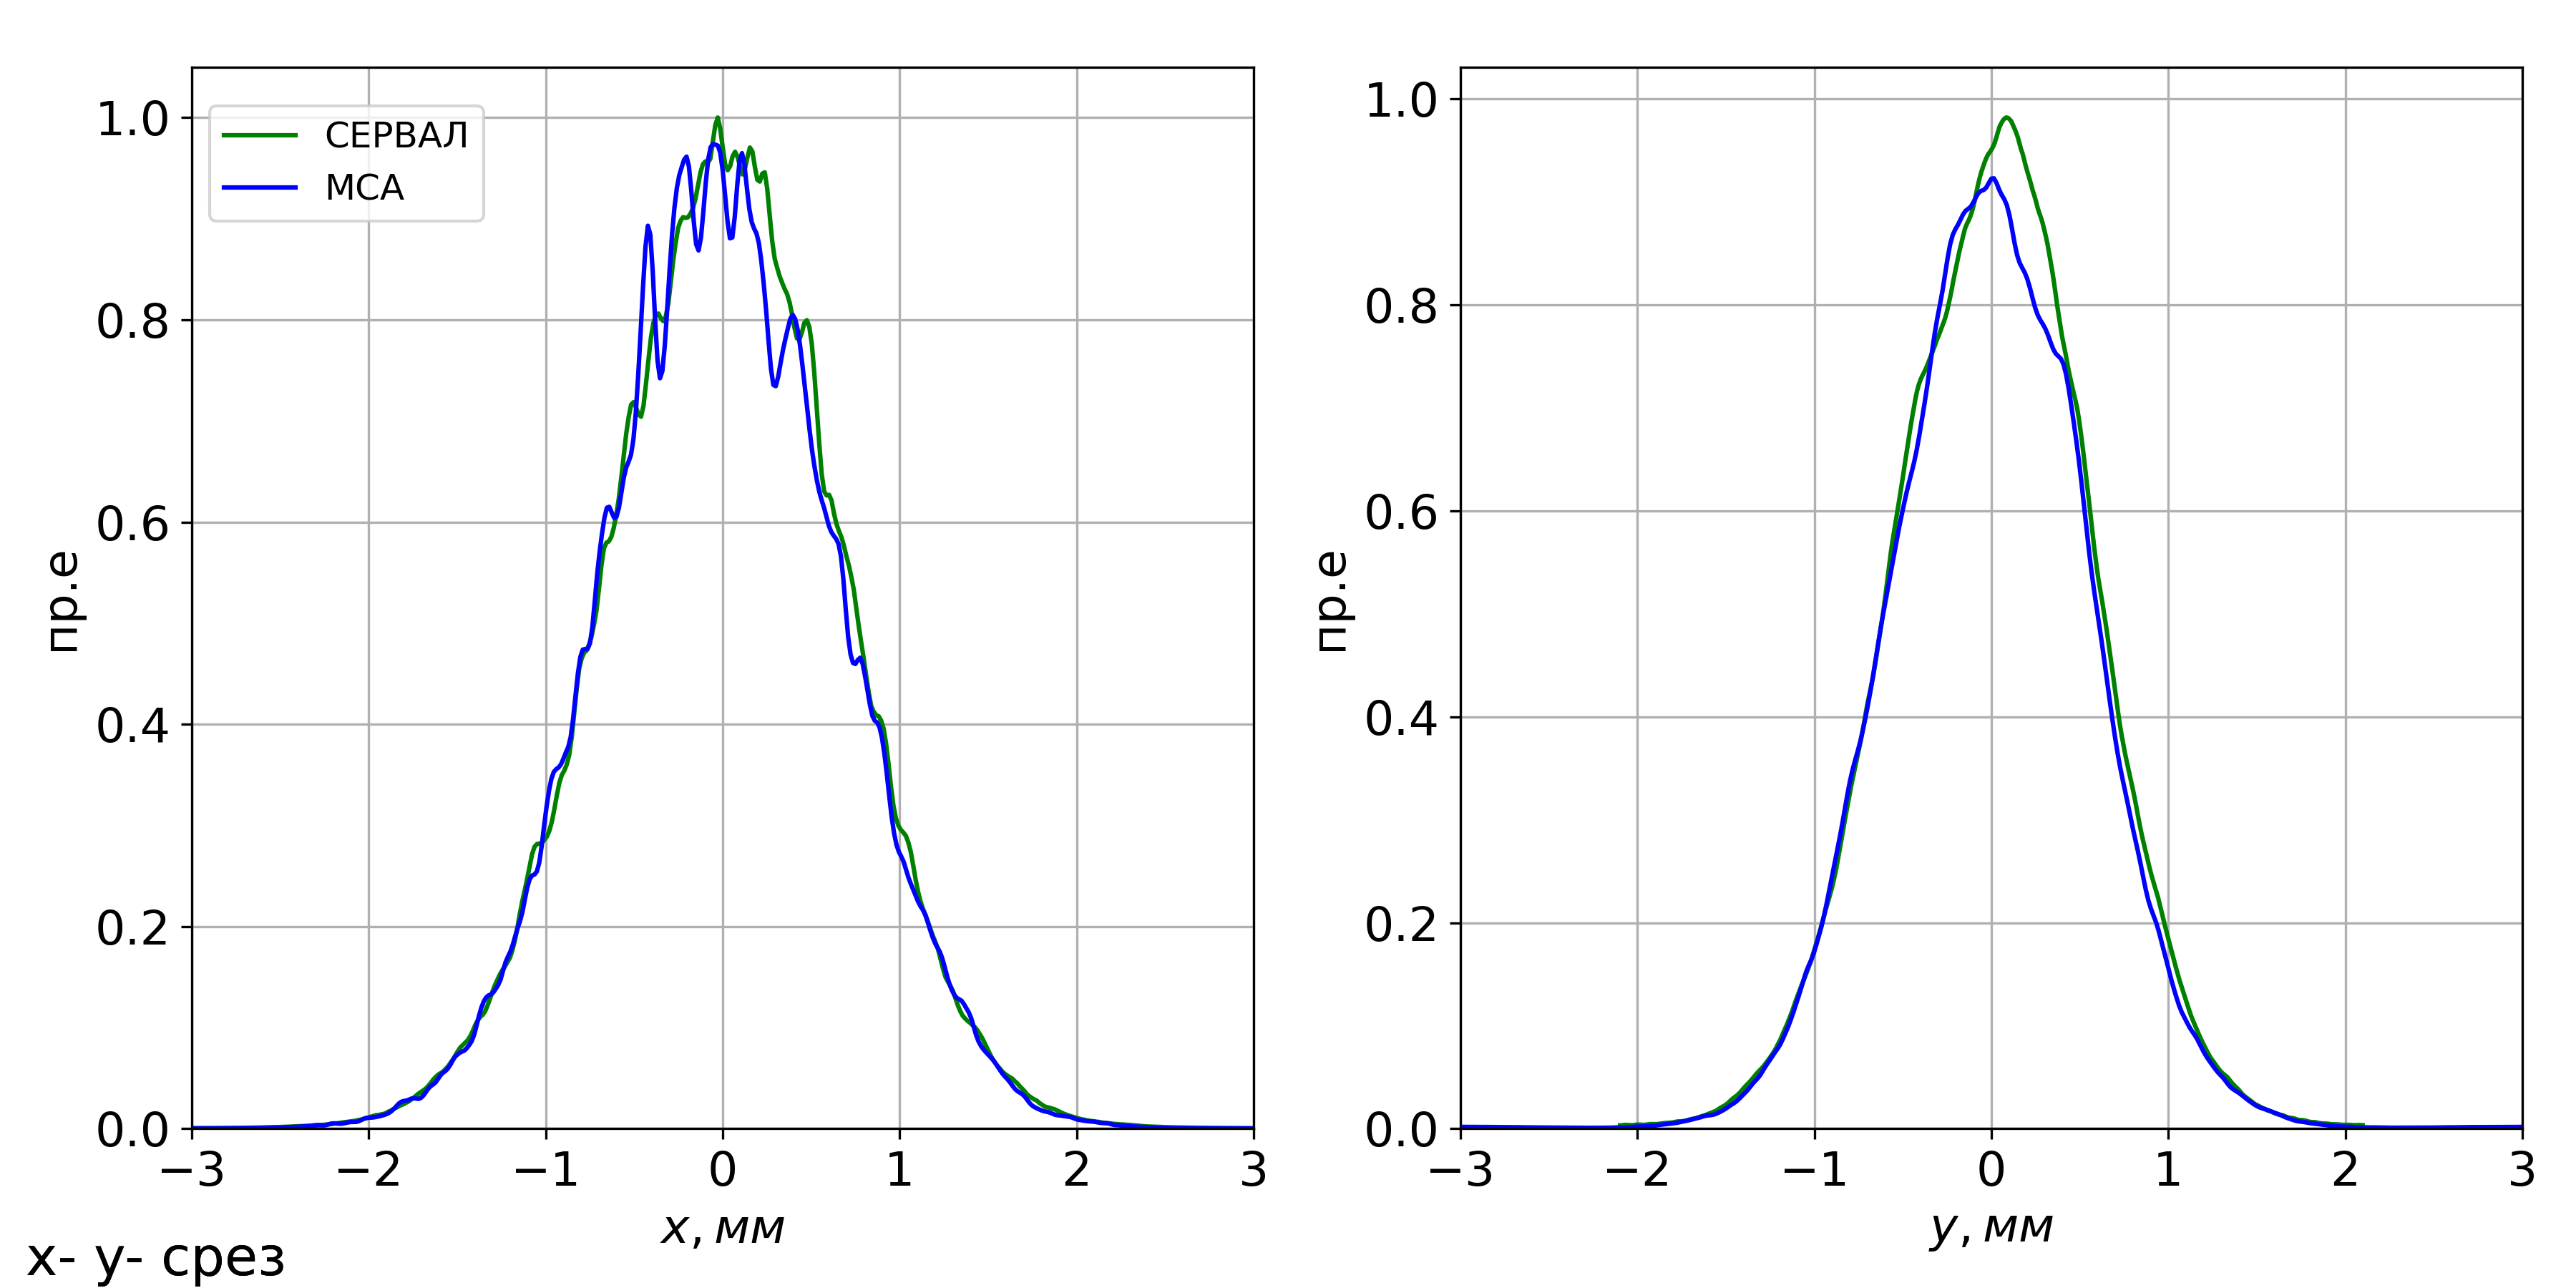
\includegraphics[width=0.99\linewidth]{SERVAL_envelopes_comparison_far_zone.png}
	\caption{Размеры излучения в дальней зоне (расходимость) на расстоянии $25$ м}
	\label{fig:SERVAL_envelopes_comparison_far_zone}
\end{figure}
В большинстве случаев можно выбирать свёртку интенсивностей по~\ref{intensity} Однако, стоит отметить, что СЕРВАЛ -- это оценочный метод и, в случае дифракционного ограниченного источника, необходимо перед проведением расчётов сделать подобный анализ подходящих распределений эффективного размера и расходимости излучения в источнике. В Приложении~\ref{AppendixA} дан подробный анализ подходящих функций для электронных сгустков с различными значениями эмиттанса.

\chapter{Применение СЕРВАЛа} \label{chapt3}
СЕРВАЛ является эффективным алгоритмом для моделирования частично когерентного синхротронного излучения. В предыдущей главе показано совпадение распределений интенсивностей излучения в дальней зоне, на источнике излучения, а также корреляционных функций, рассчитанных СЕРВАЛом, с методом сложения амплитуд, который даёт результат «из первых принципов» во всех ситуациях\footnote{необходимо помнить, что число $N_e$ должно быть достаточно велико для получения достоверного результата}. Этот сравнительный анализ свойств источника излучения показывает, что весьма ресурсозатратный по времени метод сложения амплитуд может быть заменён СЕРВАЛом без потери точности и физичности результатов. В настоящей главе приведены примеры использования СЕРВАЛа для расчёта фокусирующей системы с конечной апертурой, эксперимента Юнга и отражения частично когерентного излучения от рентгеновского зеркала с шероховатостями. 

В случае дифракционно ограниченных источников излучения, вместо СЕРВАЛа целесообразно применять метод сложения амплитуд или метод сложения интенсивностей, которые дадут сходимость за малое число реализация поля. Для СЕРВАЛа, в таком случае, потребуется тщательный анализ подходящих гладких функций, ограничивающих пространственные гармоники шума, и, строго говоря, СЕРВАЛ \textit{не моделирует} излучение электронного сгустка с бесконечно малым эмиттансом. В обратном случае источников с низкой степенью когерентности имеет смысл рассмотреть метод трассировки лучей. Для волновых методов потребуется моделировать большое число статистических реализаций поля, чтобы получить сходимость распределений к гладким функциям поперечных координат. 

В целом, прежде чем проводить оптический расчёт, необходимо изучить свойства источника излучения, например, при помощи программы SPECTRA~\cite{tanaka_spectra_2001}, где можно оценить ожидаемую степень когерентности. Только исходя из свойств источника, можно сделать выбор о наиболее предпочтительном методе моделирования. Именно такой подход даст оптимальный результат в смысле затраченного времени и достоверности полученных результатов. 

\section{Фокусирующая система с конечной апертурой}\label{section:focusing_system_with_aperture}
Оптическая схема состоит из источника излучения -- ондулятора, апертуры и фокусирующего элемента. Параметры ондулятора и электронного сгустка те же, что в Таблицах~\ref{tab:undulator_parameters} и~\ref{tab:SKIF parameters}. Размер апертуры $1 \times 1$ мм$^2$. Для СЕРВАЛа были выбраны гладкие функция поперечных координат, получающиеся в результате свёртки~\ref{intensity} Этот расчёт сопровождается сравнением результатов метода СЕРВАЛ с результатами метода сложения амплитуд.

\begin{figure}[H] 
	\centering 	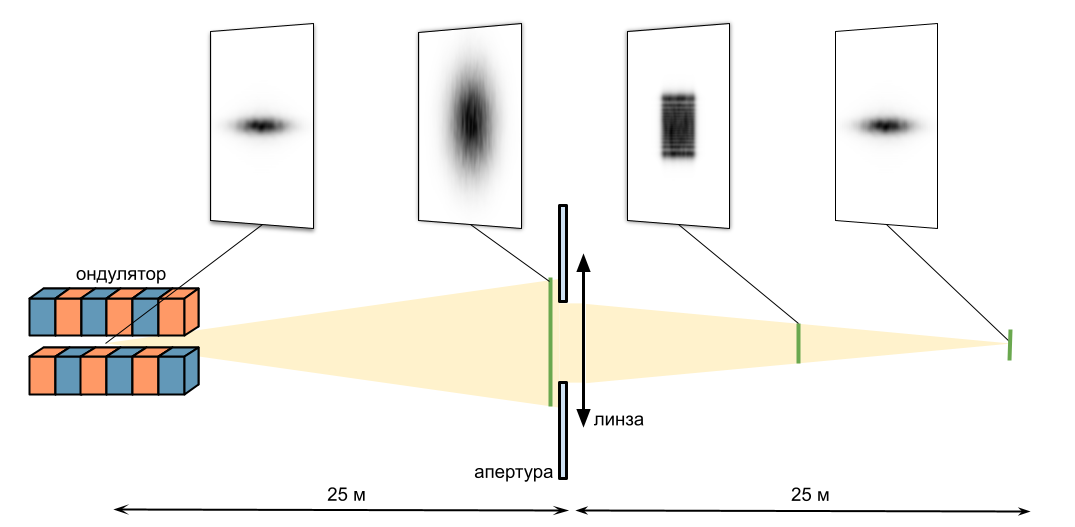
\includegraphics[width=0.99\linewidth]{beamline.png}
	\caption{Оптическая схема. Ондулятор в начале координат, апертура перед линзой на расстоянии 25 м от ондулятора, линза с фокусным расстоянием 12,5 м фокусирует излучение на образец, расположенный на 25 м от линзы. Распределения интенсивности приведены на источнике излучения, в дальней зоне перед апертурой, на половине пути к образцу и на самом образце (в фокусе).}
	\label{fig:beamline}
\end{figure}
Мнимое распределение интенсивности излучения на источнике представлено на~Рис.~\ref{fig:focusing_system_source}.
\begin{figure}[H] 
	\centering 	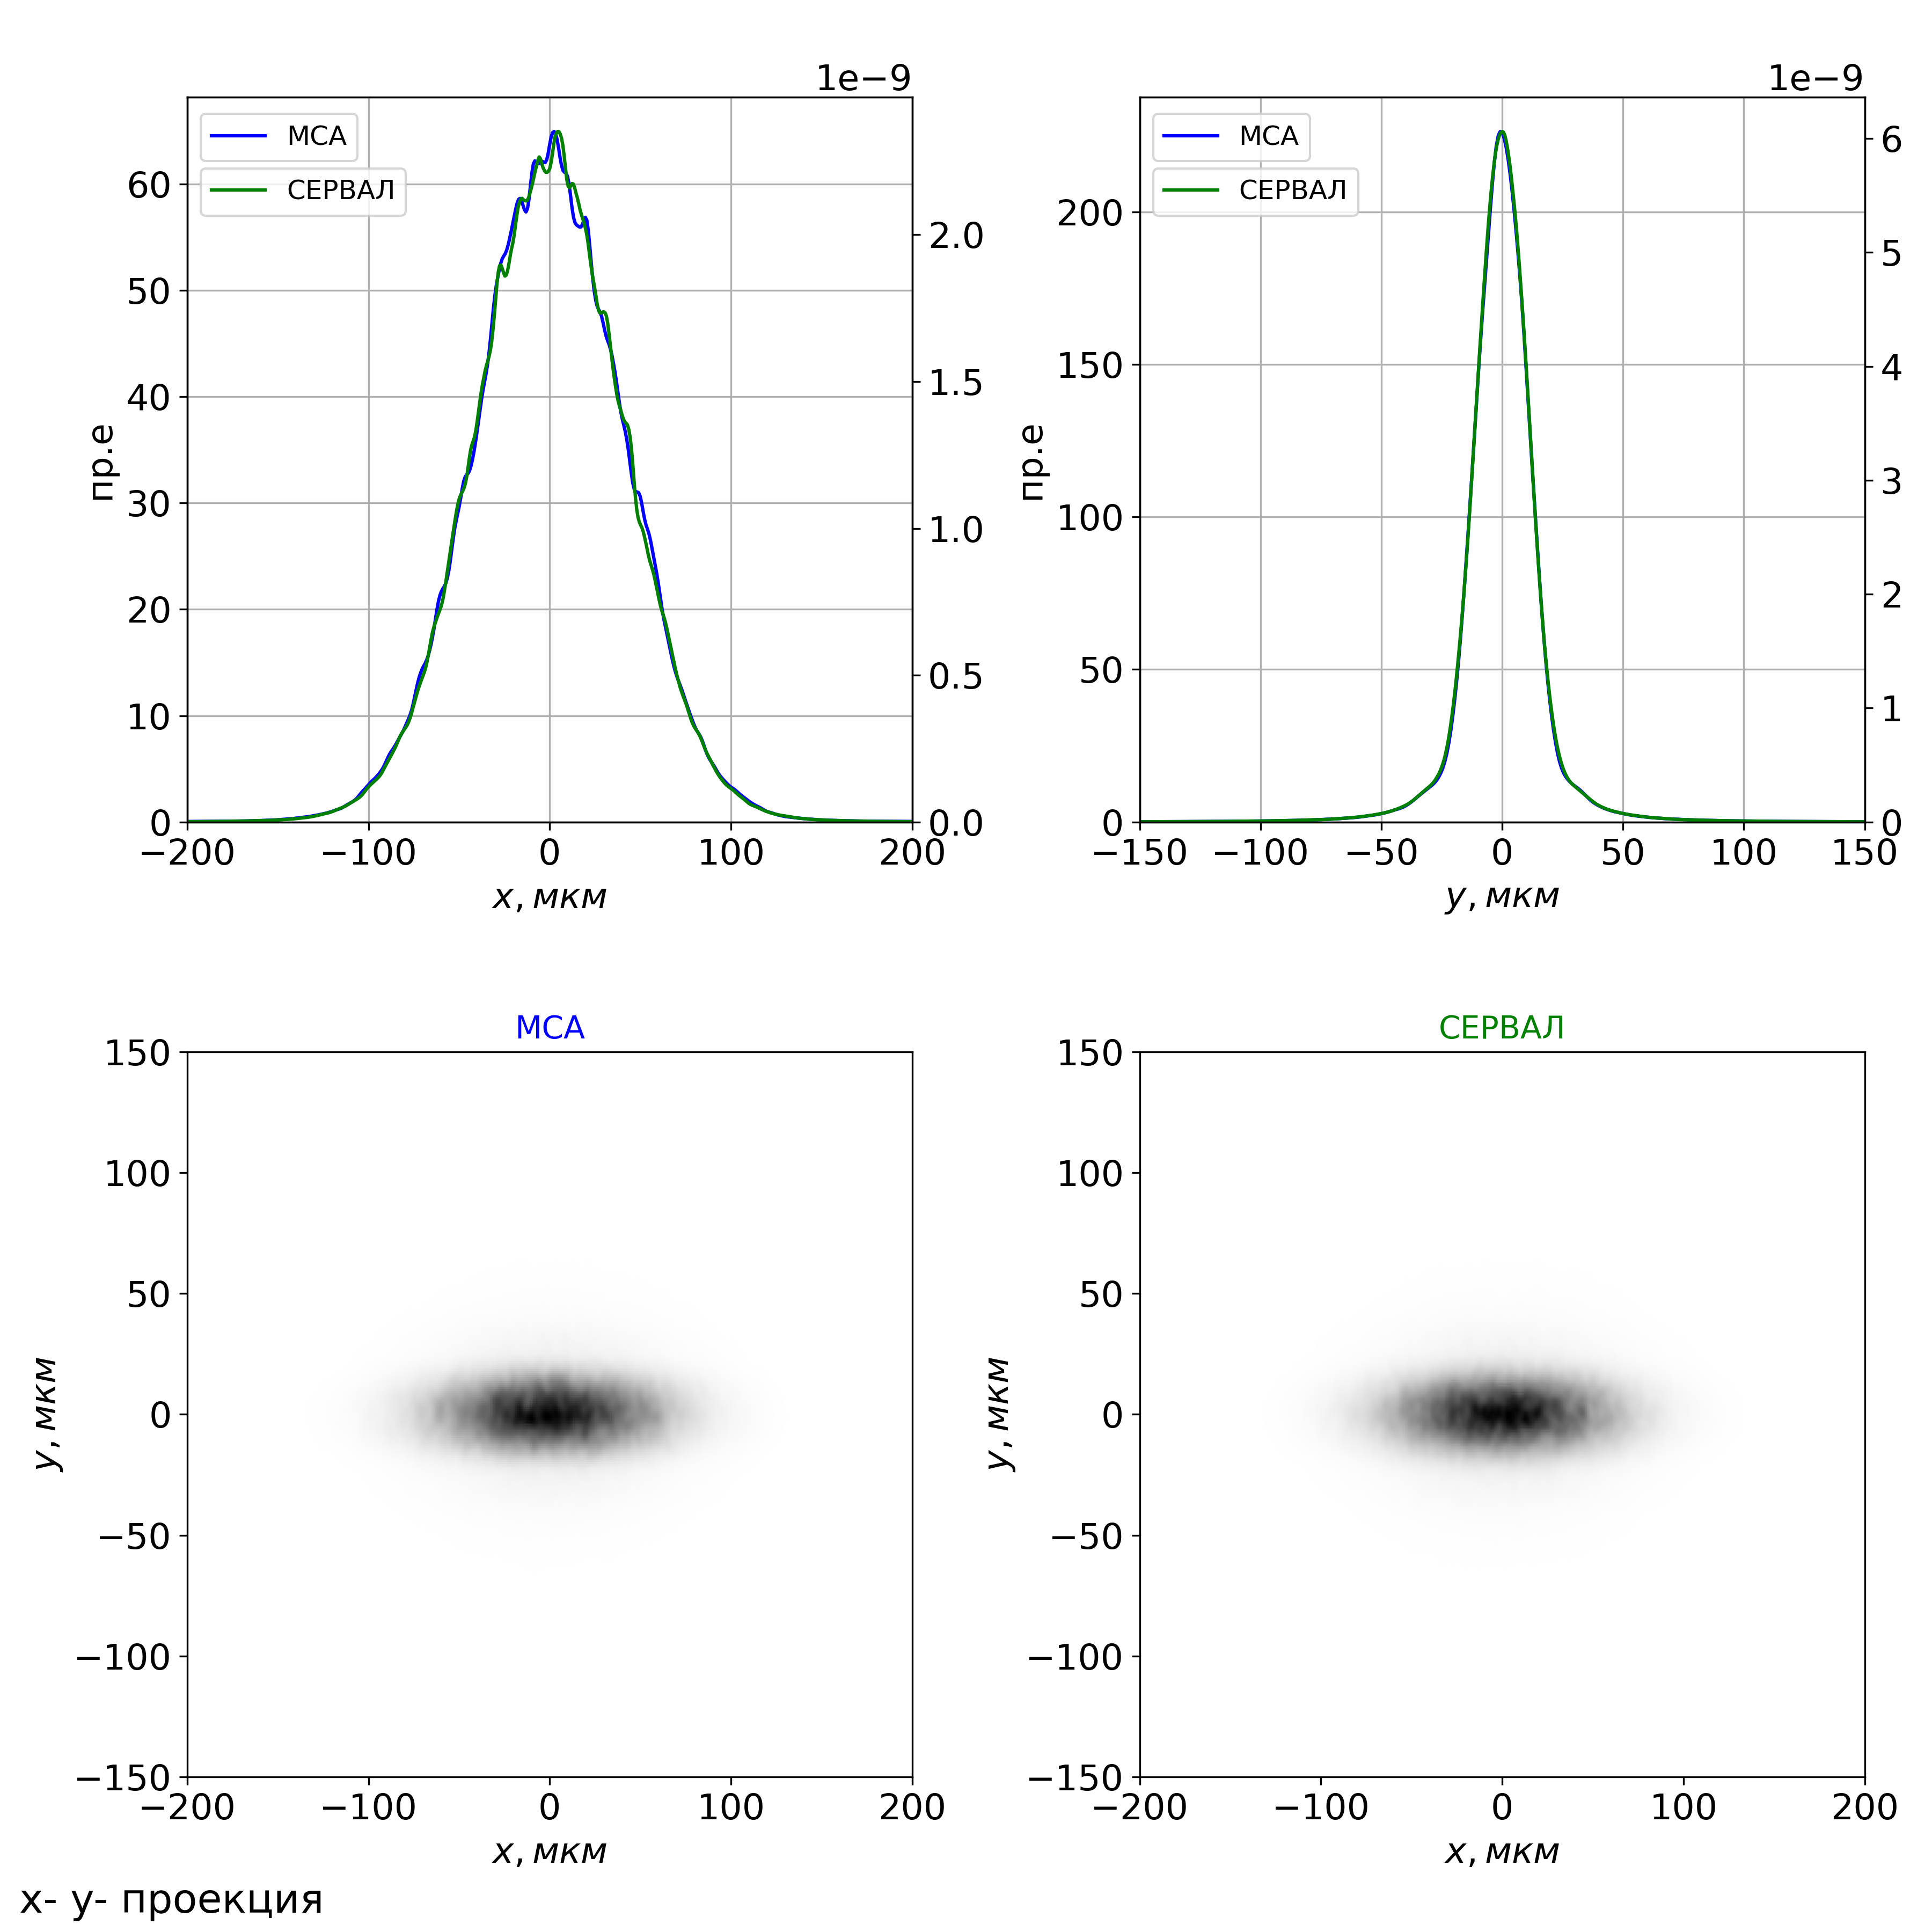
\includegraphics[width=0.99\linewidth]{0-source3.80E-05_um_4.68E-06_um_2.50E-05_urad_2.00E-05_urad_example_beamline.png}
	\caption{Распределение интенсивности на источнике излучения с величиной среднеквадратичного отклонения $40.8 \times 10.8$ мкм$^2$}
	\label{fig:focusing_system_source}
\end{figure}
\noindent Распределение поля в дальней зоне на 25 м от ондулятора представлено на Рис.~\ref{fig:focusing_system_far_zone}.
\begin{figure}[H] 
	\centering 	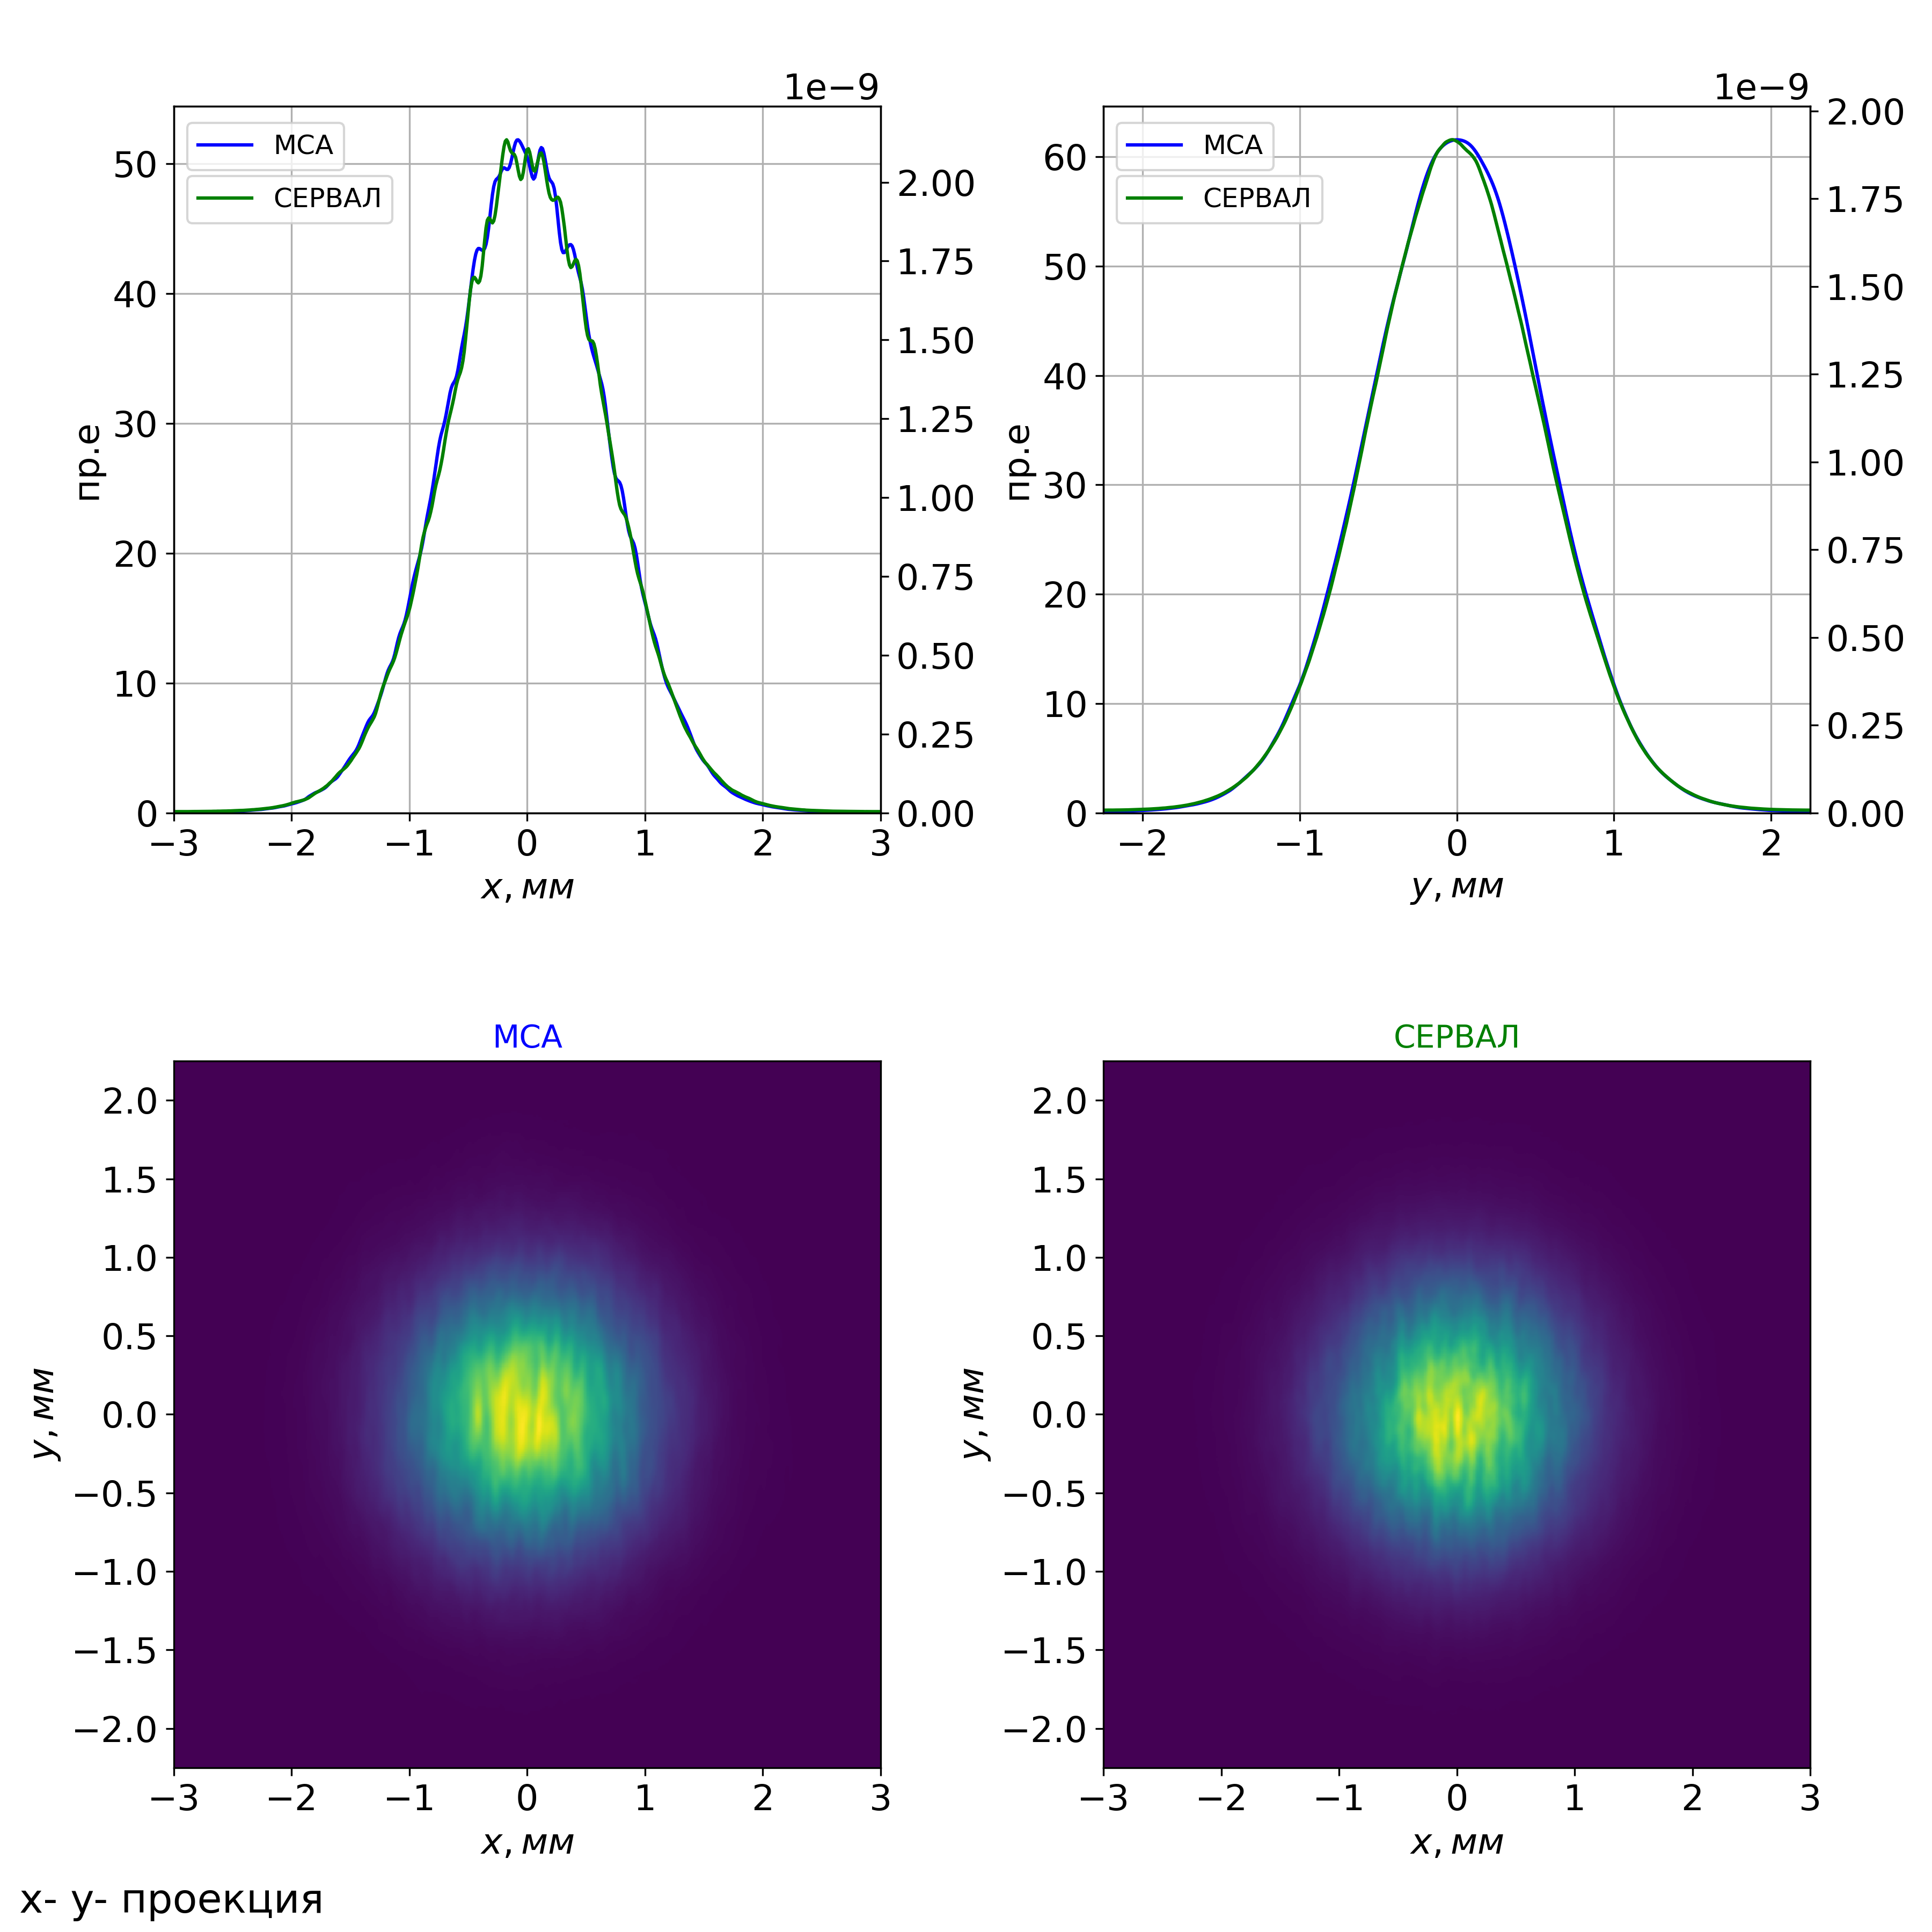
\includegraphics[width=0.99\linewidth]{1-far_zone_25_m3.80E-05_um_4.68E-06_um_2.50E-05_urad_2.00E-05_urad_example_beamline.png}
	\caption{Распределение интенсивности излучения в дальней зоне с величиной среднеквадратичного отклонения $750 \times 635$ мкм$^2$.}
	\label{fig:focusing_system_far_zone}
\end{figure}
\noindent Для усреднения было выбрано 300 статистических реализаций поля, что даёт достаточную сходимость. Однако, в структуре излучения всё ещё видны характерные спайки поля. Количество спайков в вертикальном направлении меньше, чем в горизонтальном. Их типичный размер в каждом из направлений соответствует длине поперечной когерентности. Размер пятна когерентности представлен на Рис.~\ref{fig:focusing_system_corr}.
\begin{figure}[H] 
	\centering 	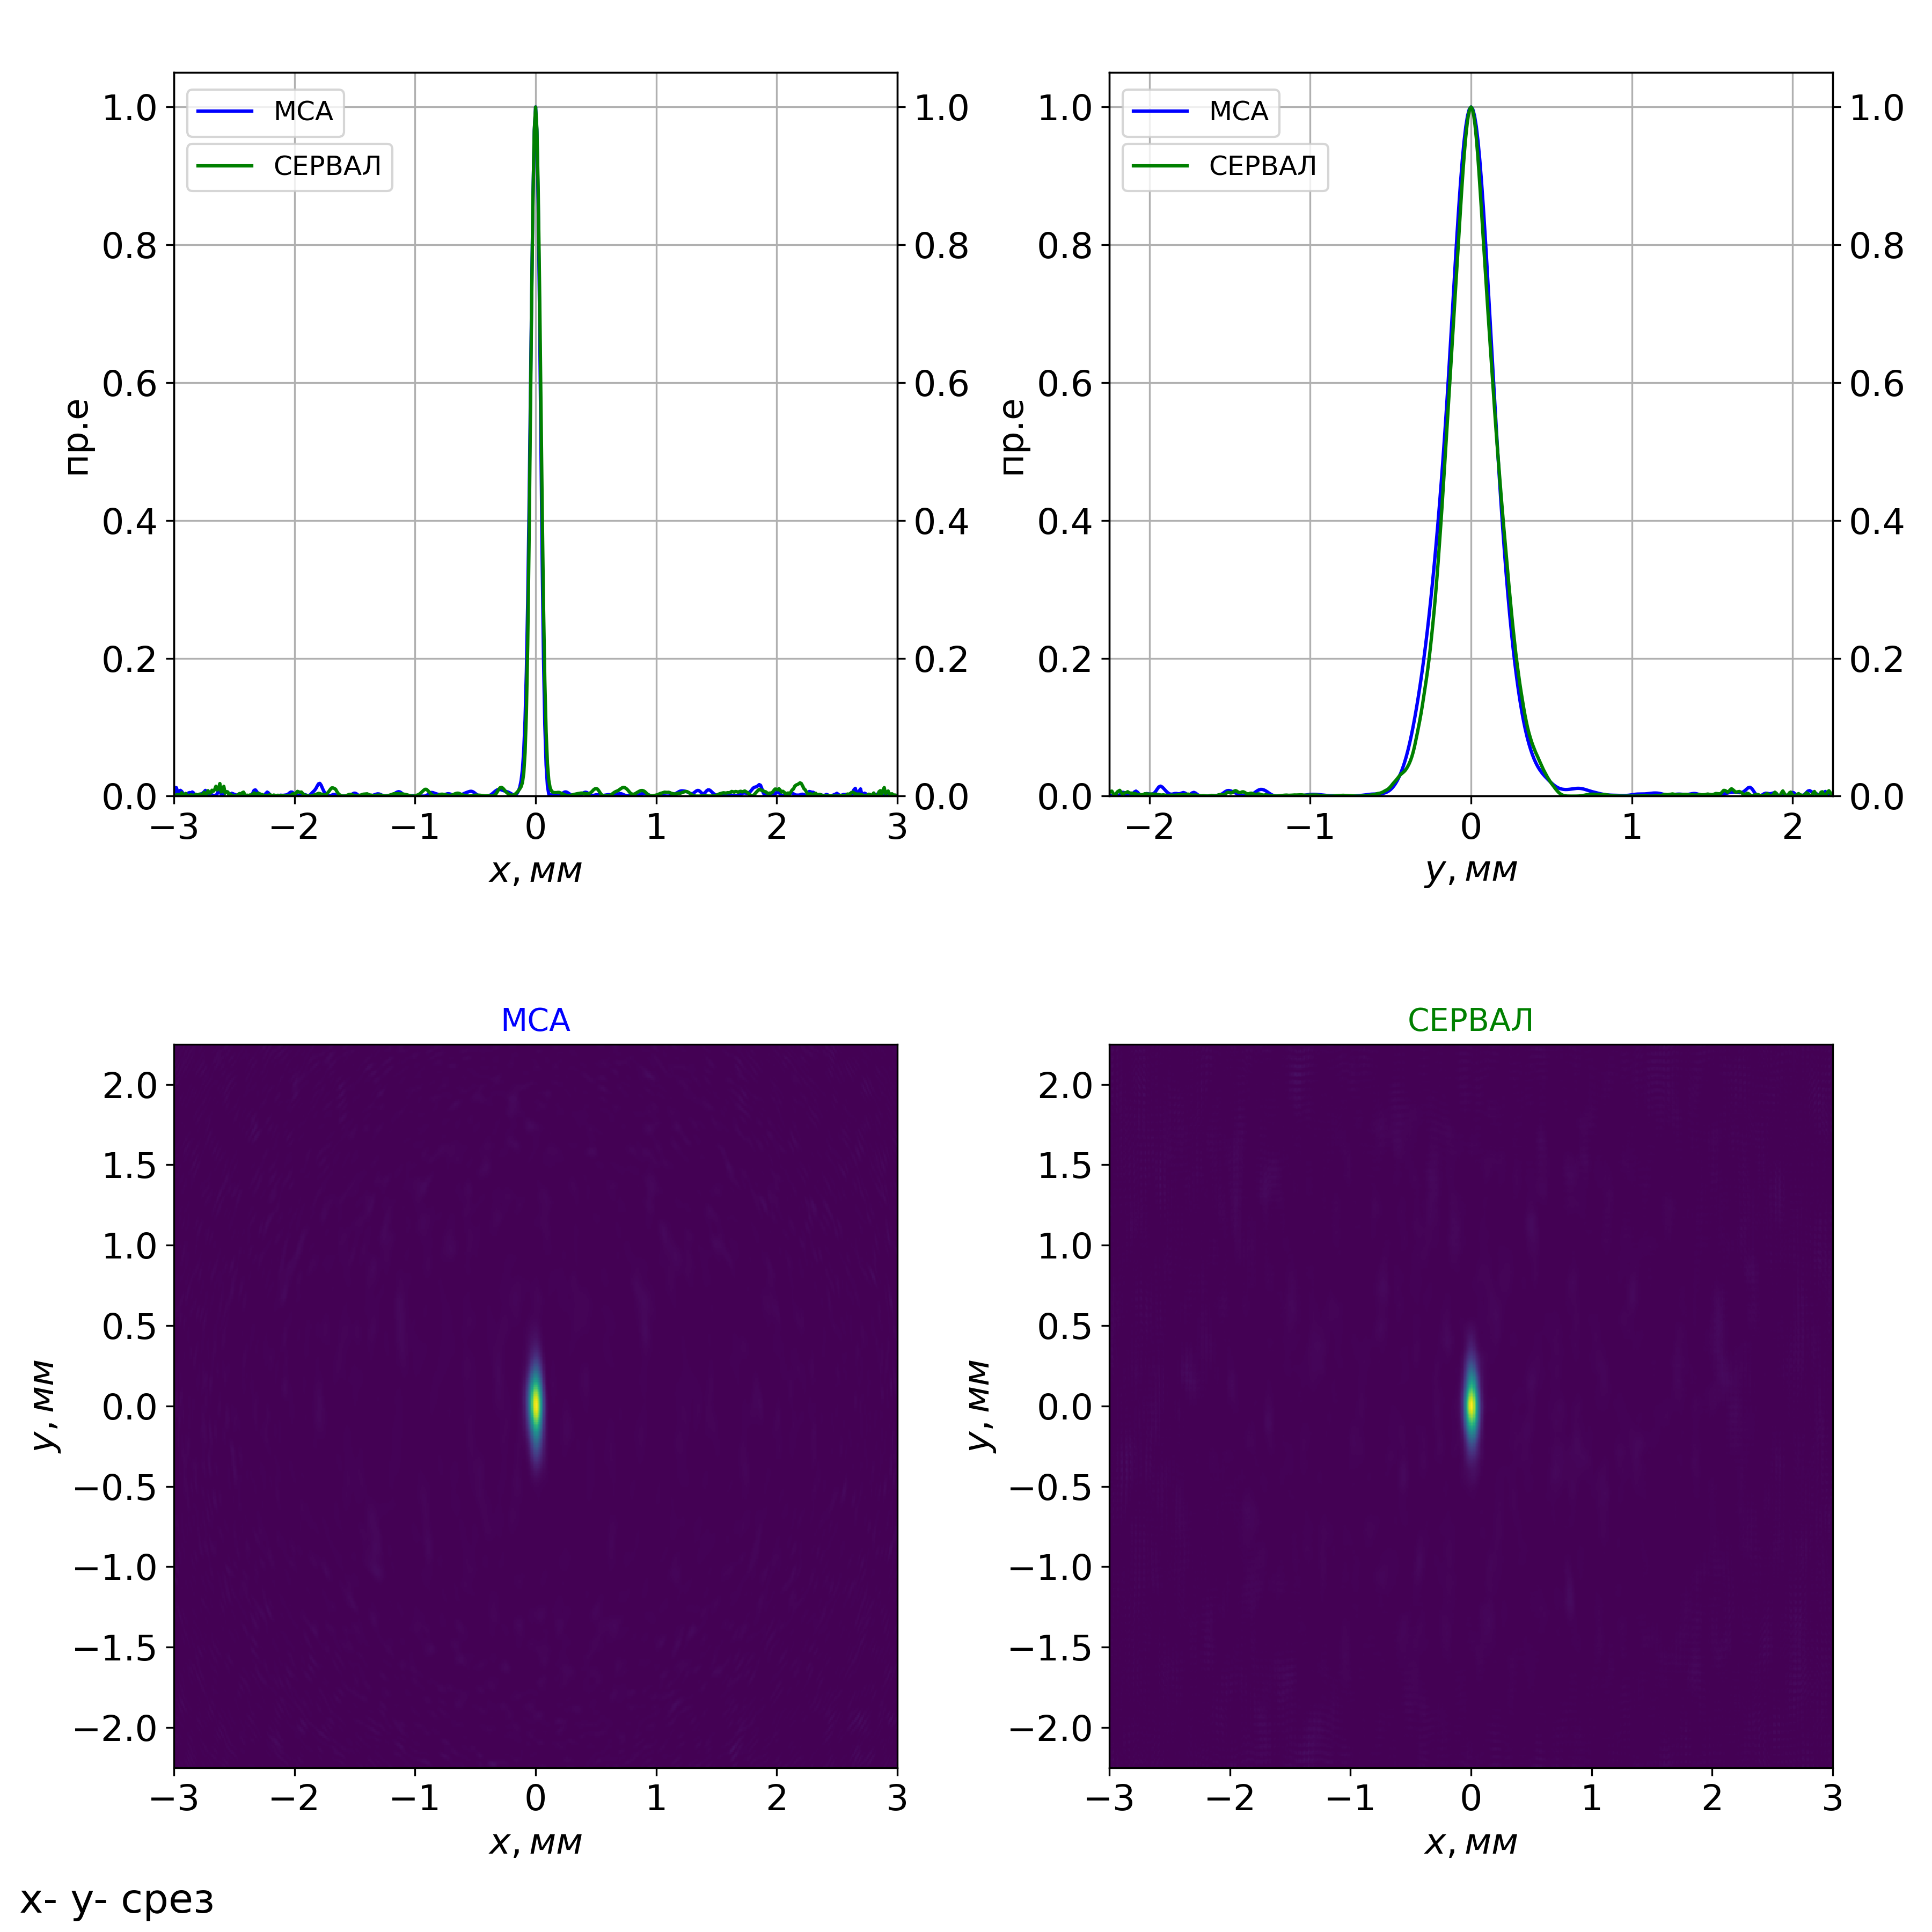
\includegraphics[width=0.99\linewidth]{corr3.80E-05_um_4.68E-06_um_2.50E-05_urad_2.00E-05_urad_example_beamline.png}
	\caption{Распределение функции взаимной когерентности, построенное по формуле~\ref{eq:g1} с величиной среднеквадратичного отклонения $40 \times 150 $ мкм$^2$.}
	\label{fig:focusing_system_corr}
\end{figure}
\noindent Распределение интенсивности поля после дифракции на апертуре и $12,5$ м распространения поля через пустое пространство приведено на Рис.~\ref{fig:focusing_system_after_aperture}.
\begin{figure}[H] 
	\centering 	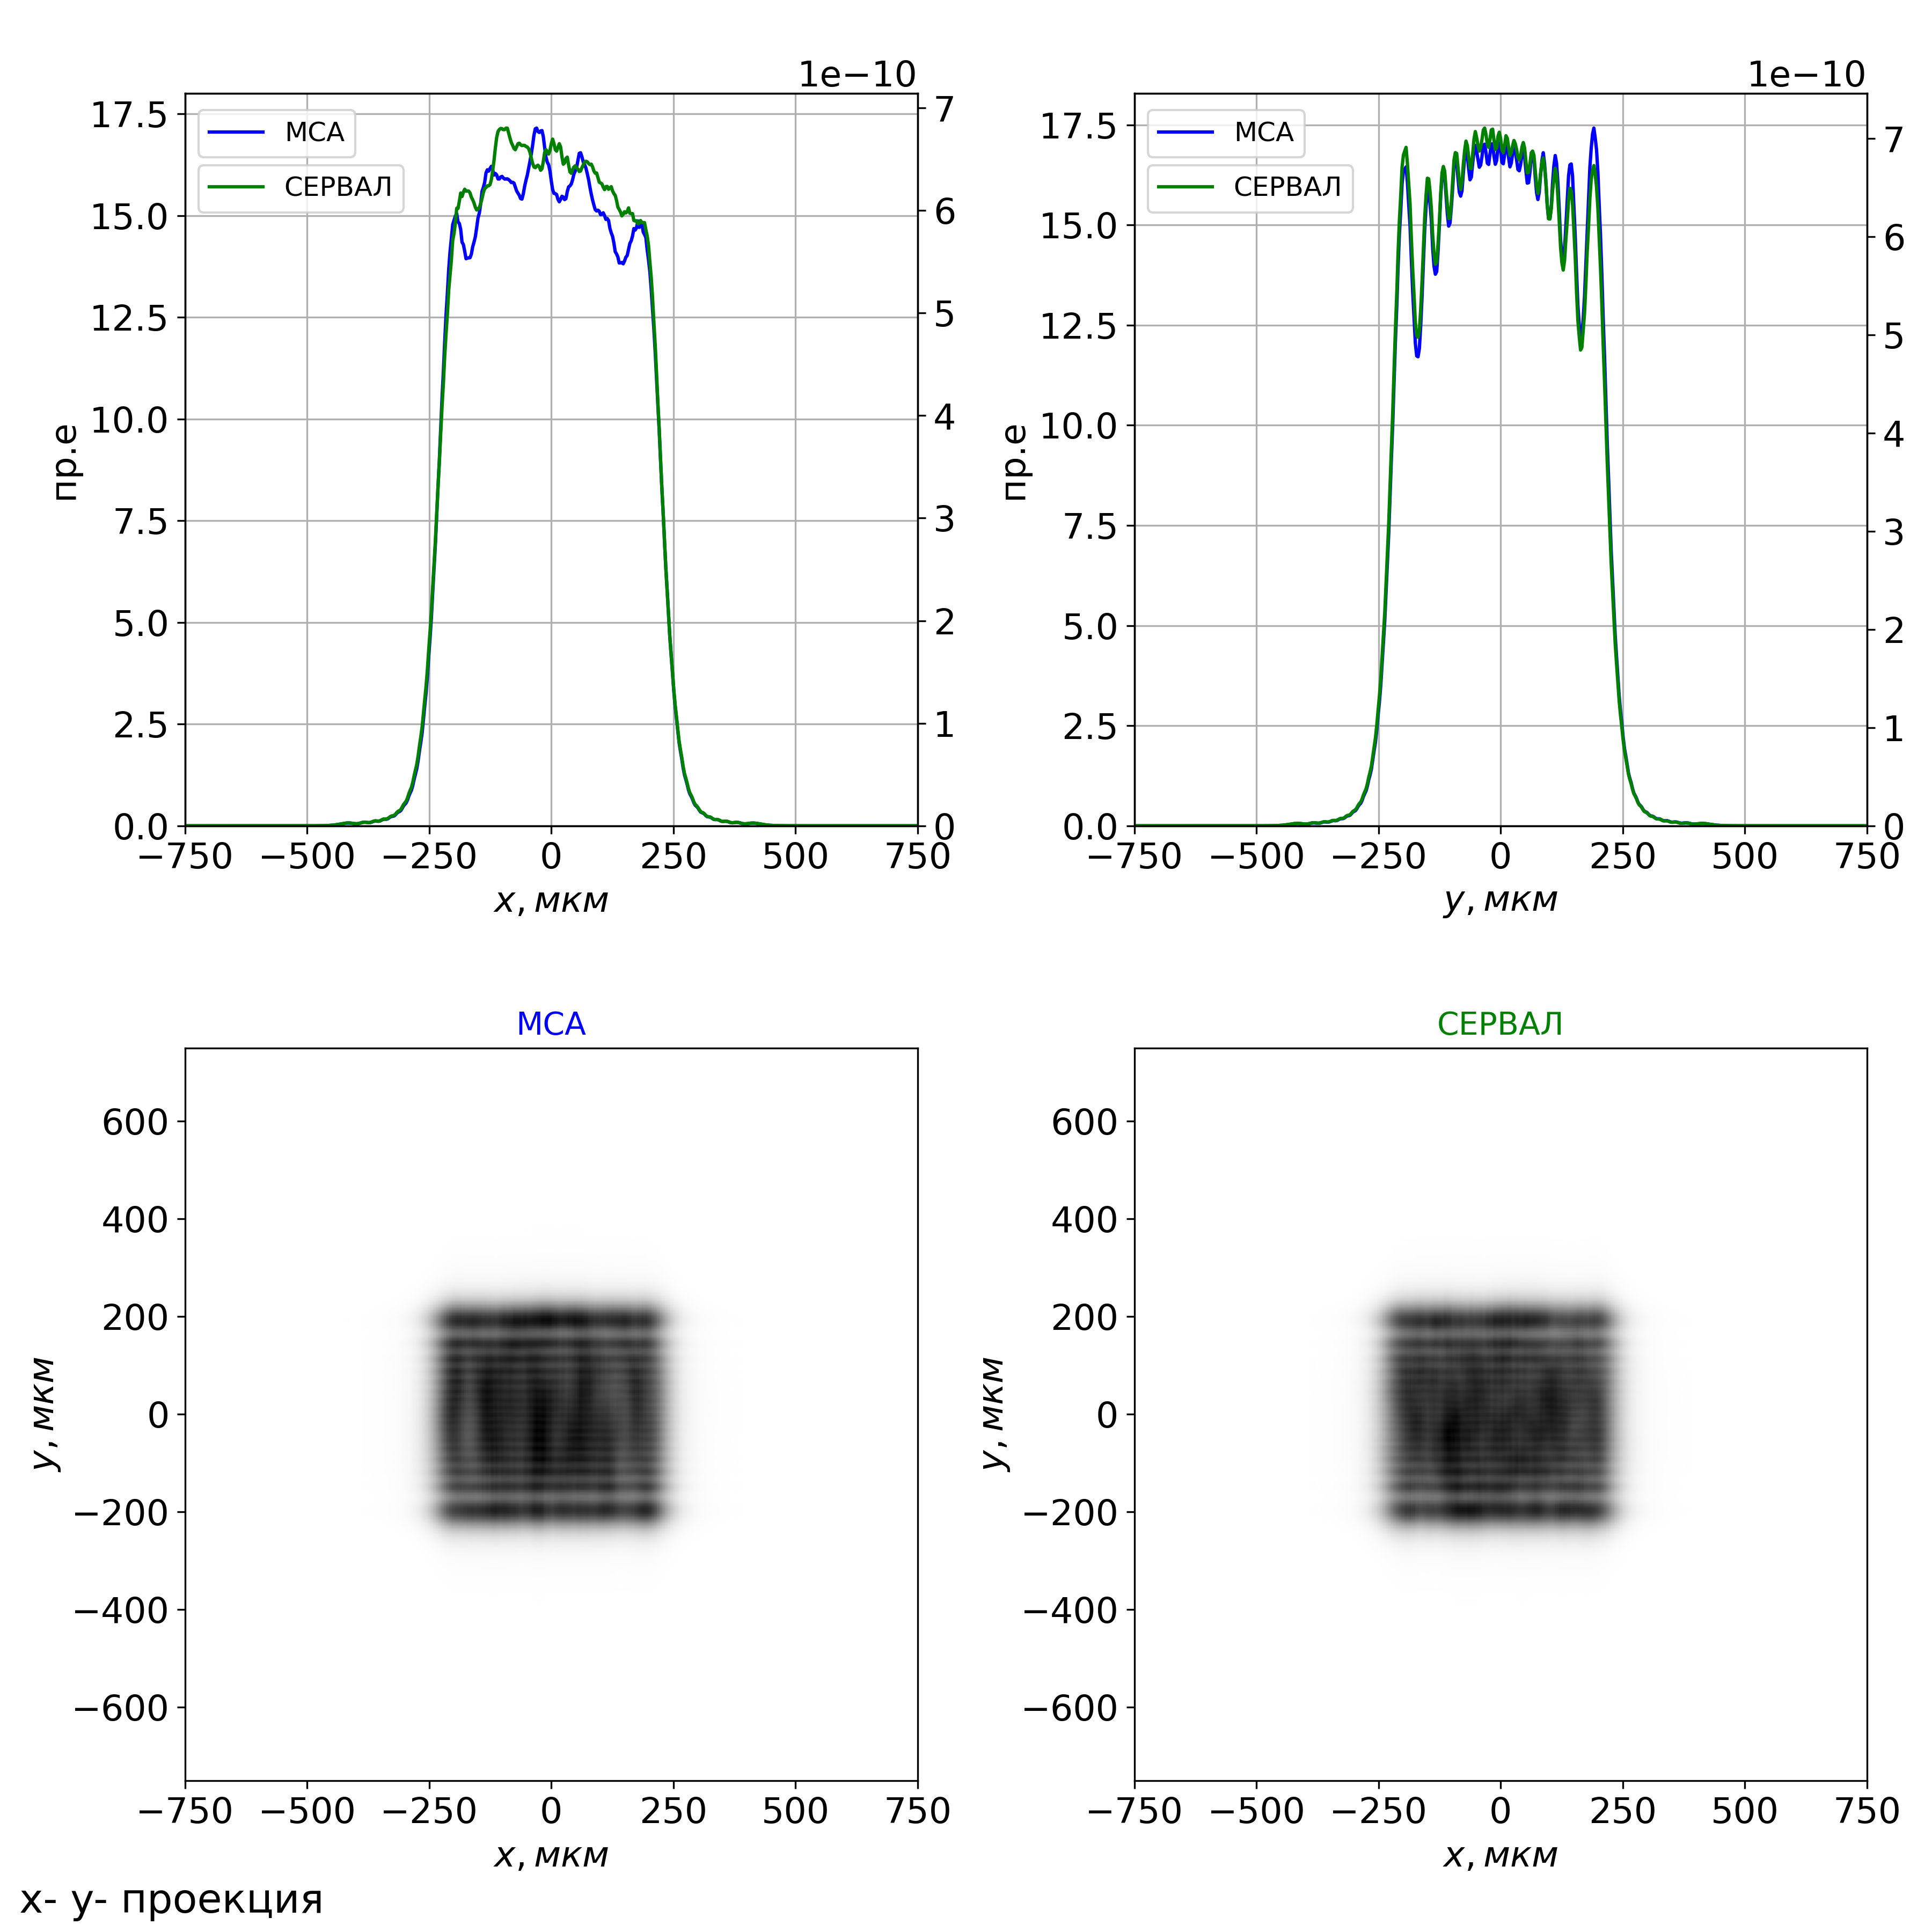
\includegraphics[width=0.99\linewidth]{2-far_zone_12_5_m_after_aperture3.80E-05_um_4.68E-06_um_2.50E-05_urad_2.00E-05_urad_example_beamline.png}
	\caption{Результат дифракции на апертуре и 12.5 м распространения через пустое пространство, величина среднеквадратичного отклонения представленных распределений $225 \times 222$ мкм$^2$}
	\label{fig:focusing_system_after_aperture}
\end{figure}
\noindent Дифракционные картины отличаются для каждого из направлений: для вертикального дифракционные пики более выраженные ввиду большей длины когерентности, для горизонтального направления заметен только первый дифракционный максимум из-за заметно меньшей степени когерентности.

Распределение поля на образце (в фокусе оптической системы) приведено на Рис.~\ref{fig:focusing_system_in_focus}.
\begin{figure}[H] 
	\centering 	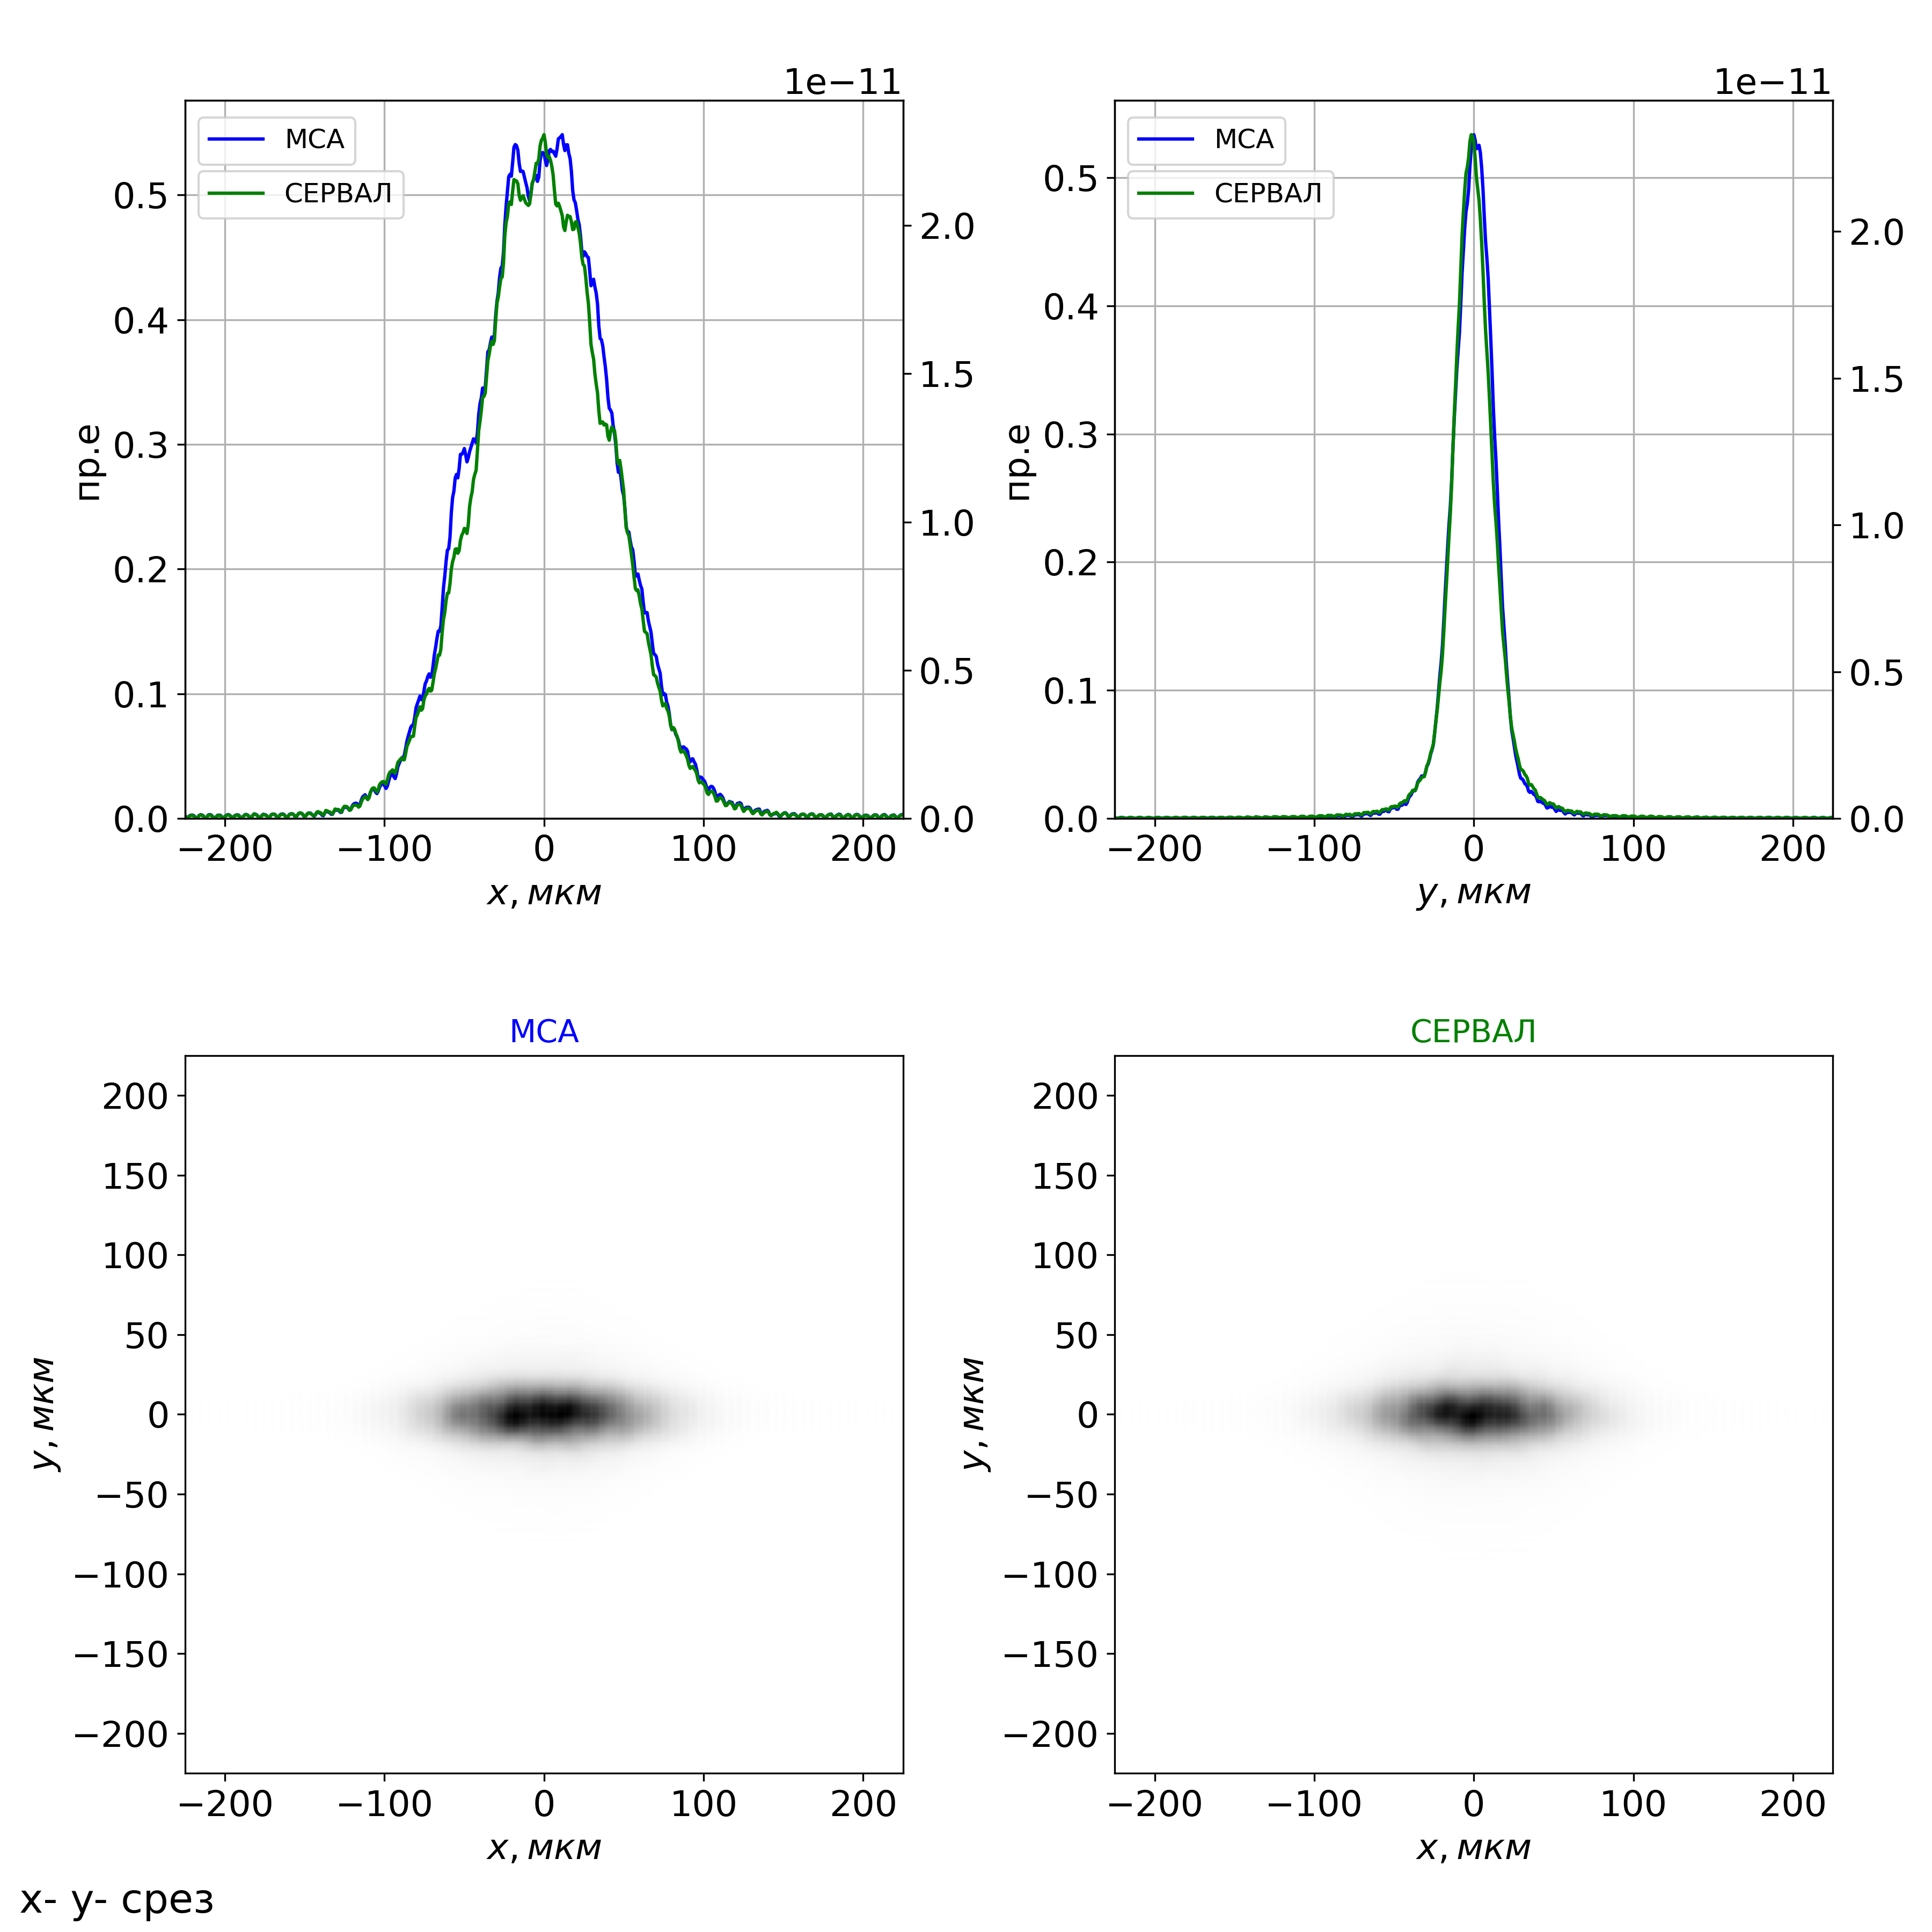
\includegraphics[width=0.99\linewidth]{3-70_m_focal_plane3.80E-05_um_4.68E-06_um_2.50E-05_urad_2.00E-05_urad_example_beamline.png}
	\caption{Распределение излучения в фокусе, величина среднеквадратичного отклонения представленных распределений $42 \times 13,5$ мкм$^2$}
	\label{fig:focusing_system_in_focus}
\end{figure}
\noindent Для моделирования было выбрано соотношение плеч фокусирующей системы -- $1:1$. По критерию Рэлея, при размере апертуры $1 \times 1$ мм$^2$ угловая разрешающая способность такой системы $\theta_{diff} = 1,22 \lambda / D  = 0,7$ мкрад, где $D$ размер апертуры. Угловой размер источника излучения $\theta_{source}$ для каждого из направлений $3,26 \times 0,86$ мкрад$^2$. Размер изображения в фокусе определяется как: $\sigma = b\sqrt{\theta^2_{source} +  \theta^2_{diff}}$, где $b$ -- расстояние от линзы до фокальной плоскости. Величины среднеквадратичного отклонения для такой оценки: в горизонтальном направлении $42$ мкм и в вертикальном направлении $14$ мкм, что согласуется с результатами моделирования, представленными на Рис.~\ref{fig:focusing_system_in_focus}.  
\section{Интерференционный эксперимент}
Для наглядной демонстрации эффектов, связанных с частичной когерентностью, показательно провести классический опыт Юнга (двухщелевой интерферометр Юнга). Ниже на Рис.~\ref{fig:double_slit_size_corr} приведён размер излучения на $25$ м от источника и распределение корреляционной функции в увеличенном масштабе. Щели на рис~\ref{fig:double_slit_size_corr} обозначены разными цветами: зелёный цвет -- межщелевой зазор $75$ мкм, красный -- $150$ мкм и оранжевый -- $300$ мкм, при среднеквадратичном отклонении функции поперечной когерентности $40 \times 150$ $\textup{мкм}^2$. 
\begin{figure}[H]
	\centering
	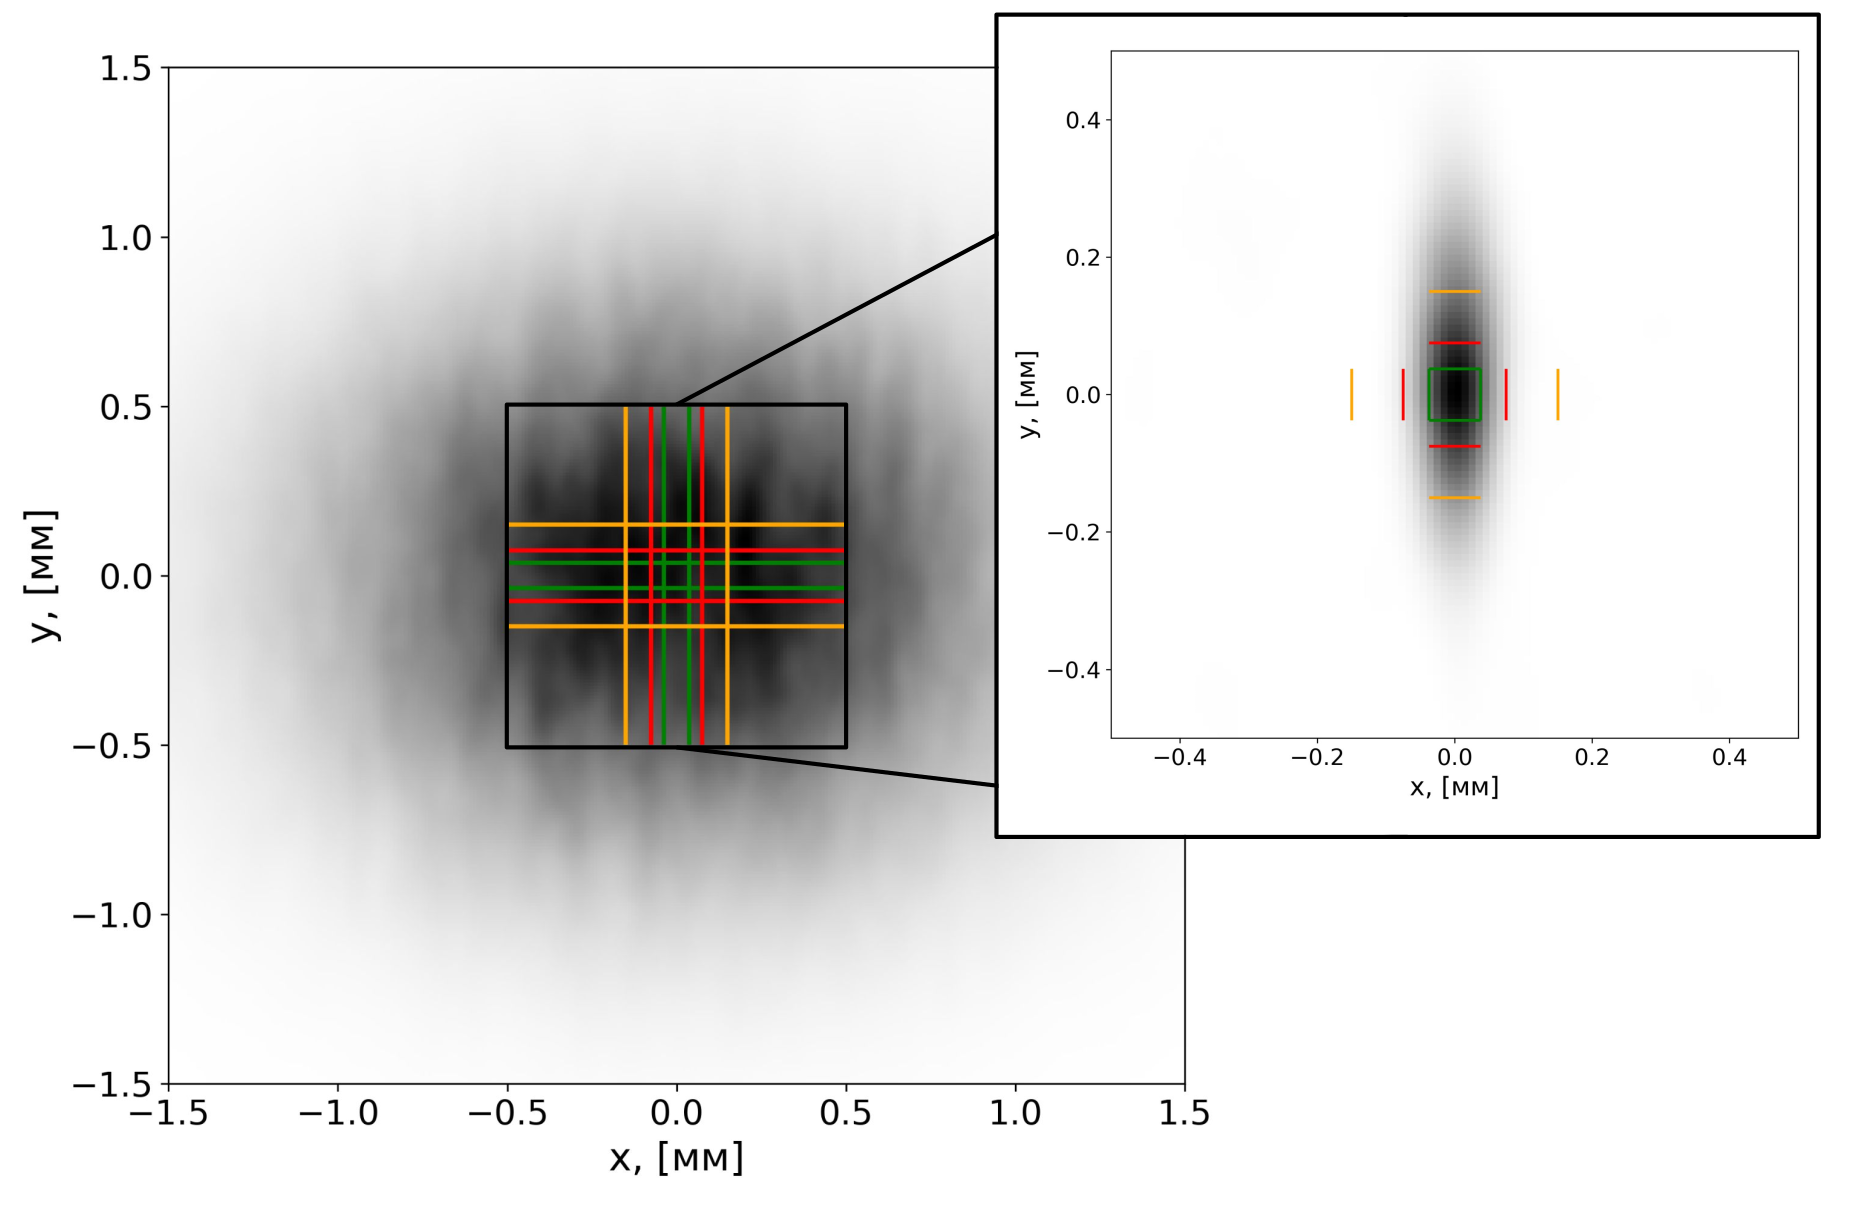
\includegraphics[width=0.75\linewidth]{double_slit_size_corr.png}
	\caption{Размер излучения на $25$ м от источника (слева) и пятно когерентности на $25$ м от источника с щелями (справа), щели обозначены цветными полосками. Три набора щелей для каждого из направлений. Межщелевые расстояния: зелёные полоски -- $75$ мкм, красные -- $150$ мкм и оранжевые -- $300$ мкм.}
	\label{fig:double_slit_size_corr}
\end{figure}
\noindent Схема эксперимента представлена на Рис.~\ref{fig:double slit experiment}.
\begin{figure}[H] 
	\centering 	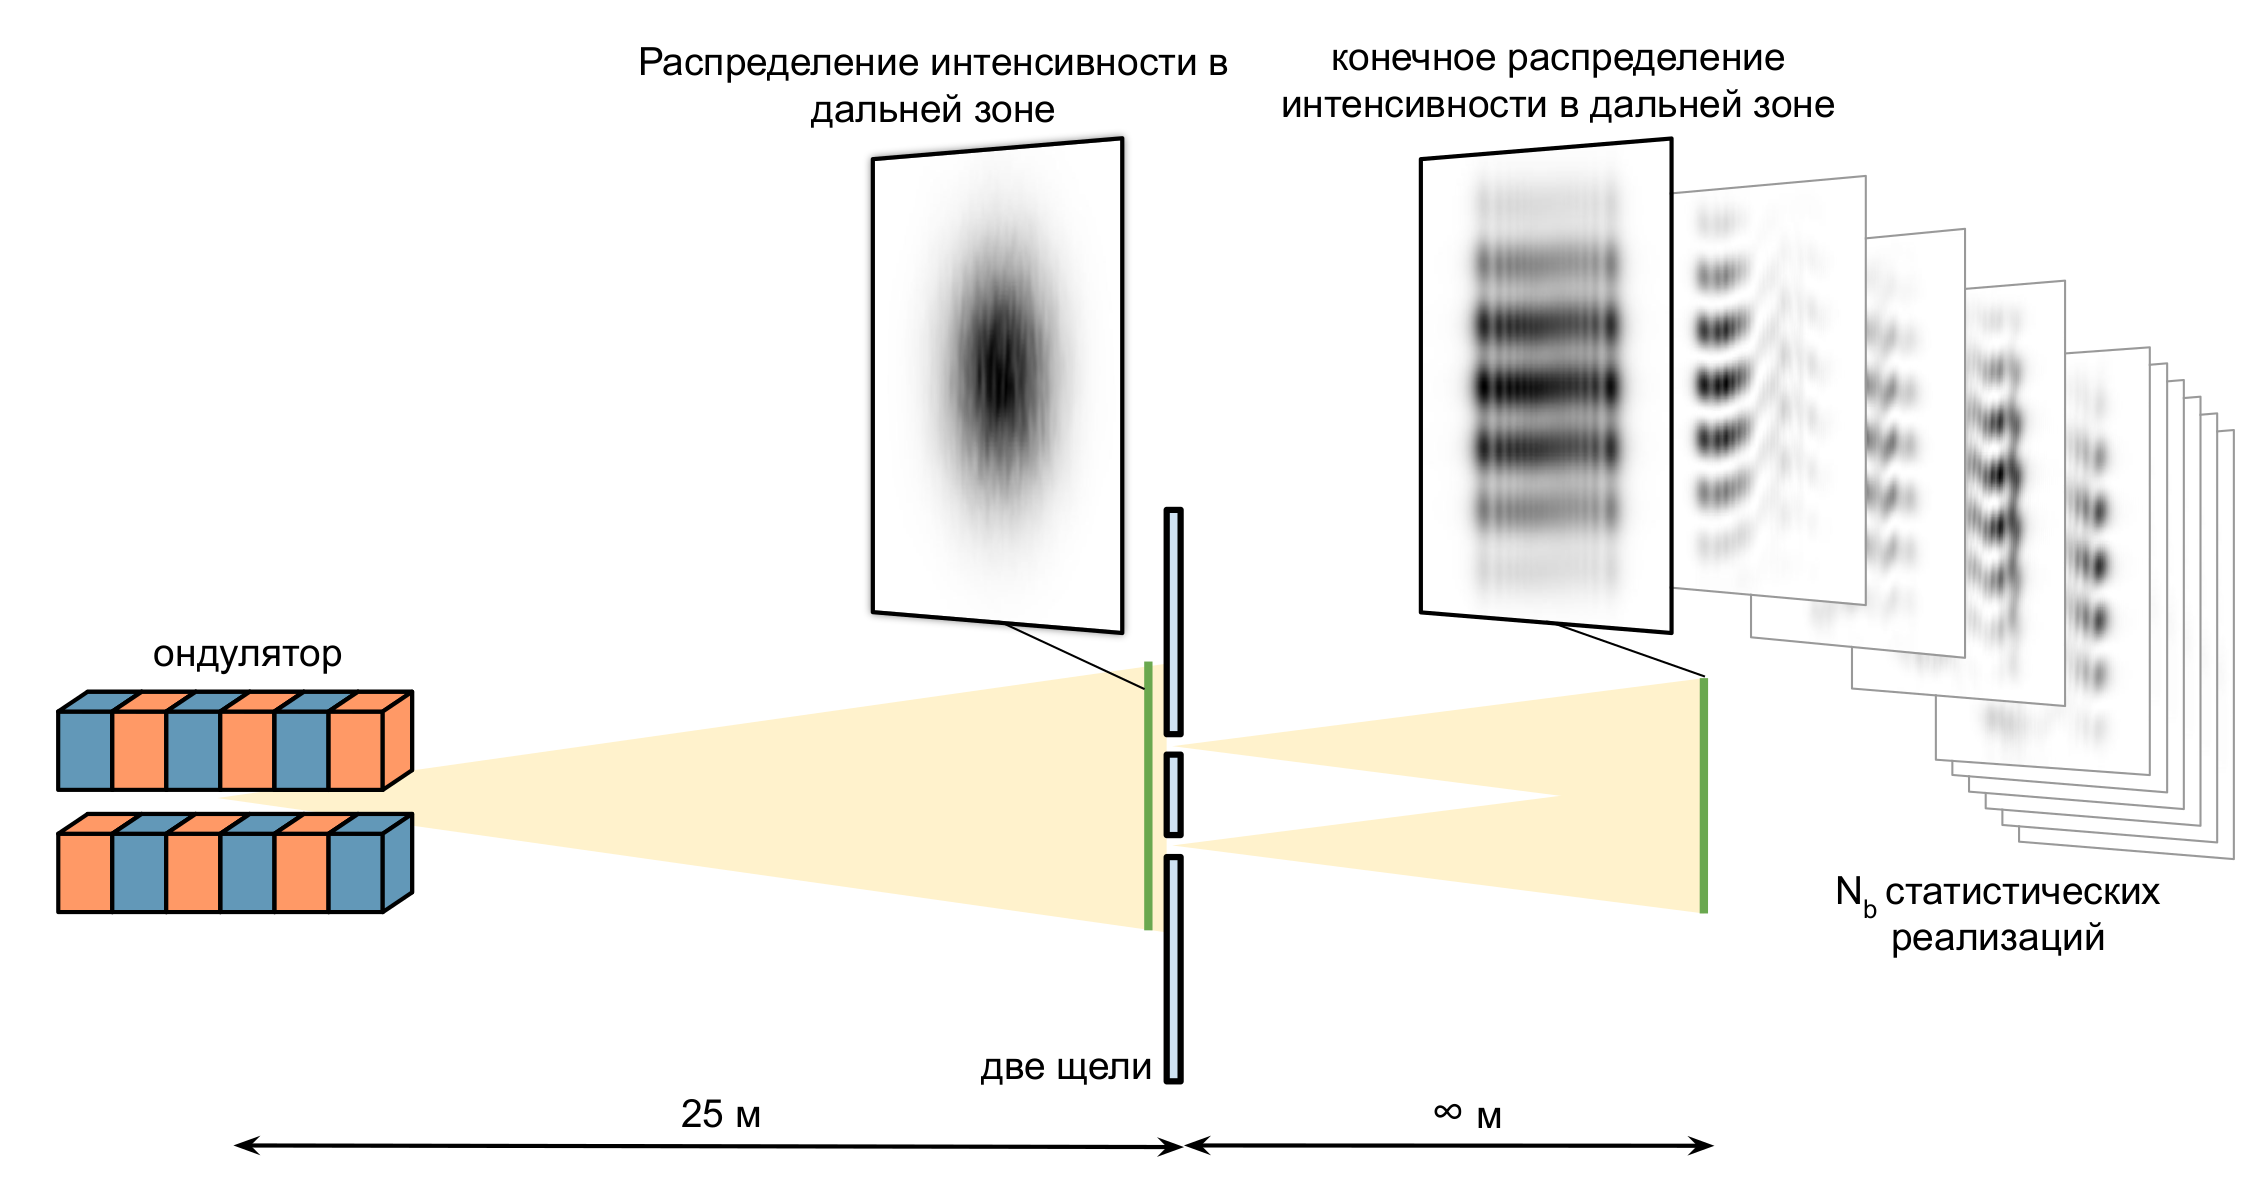
\includegraphics[width=0.99\linewidth]{double_slit_scheme.png}
	\caption{Схема двухщелевого эксперимента. После щелей -- интерферограмма усреднённа по 400 реализациям, за ней представлены интерферограммы для отдельных реализаций из статистического набора. Интерферограммы приведены в дальней зоне. Примечательно, что видность каждой из реализаций после дифракции на щелях равна единице~\cite{goodman_statistical_2015}, но при усреднении по многим реализациям видность падает из-за наличия частичной когерентности излучения.}
	\label{fig:double slit experiment}
\end{figure}
\noindent Интерферограммы для различных межщелевых расстояний показаны на Рис.~\ref{fig:x_slits_75},~\ref{fig:x_slits_150},~\ref{fig:x_slits_300}. Распределения представлены для \textit{вертикального} расположения щелей.
\begin{figure}[H]
	\centering
	\begin{subfigure}{0.33\textwidth}
		\centering
		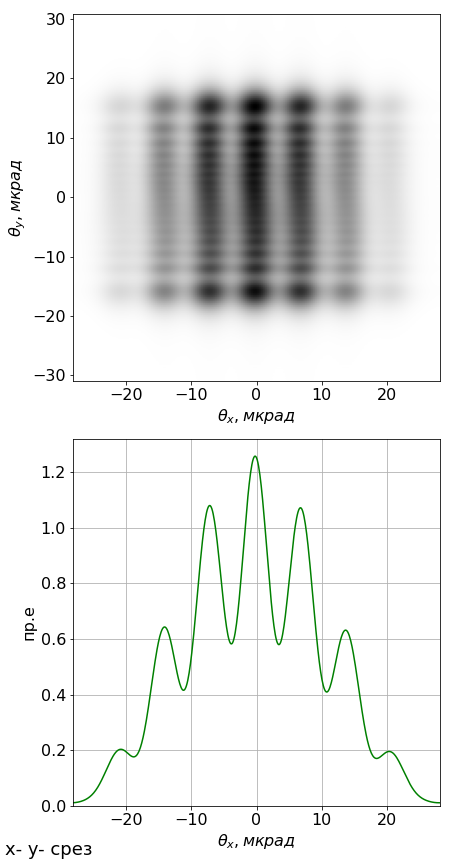
\includegraphics[width=1\linewidth]{x_slits_width_3e-05_separation_7.5e-05_.png}
		\caption{}
		\label{fig:x_slits_75}
	\end{subfigure}
	\begin{subfigure}{0.33\textwidth}
		\centering
		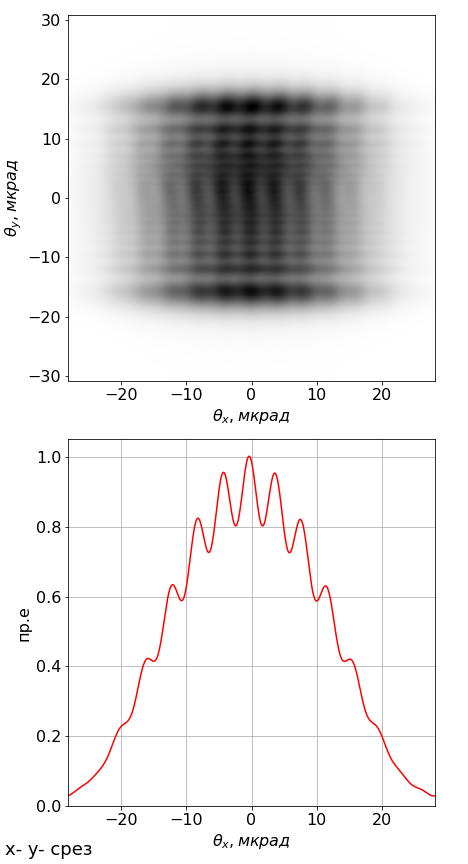
\includegraphics[width=1\linewidth]{x_slits_width_3e-05_separation_0.00015_.png}
		\caption{}
		\label{fig:x_slits_150}
	\end{subfigure}\hfill
	\begin{subfigure}{0.33\textwidth}
		\centering
		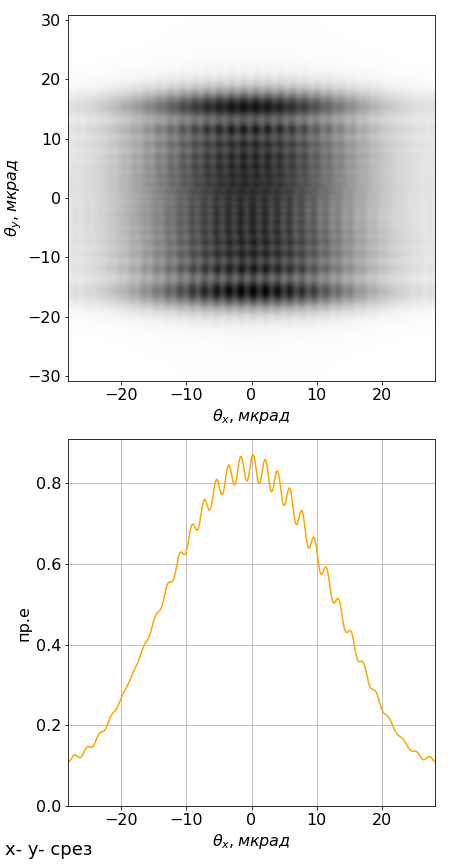
\includegraphics[width=1\linewidth]{x_slits_width_3e-05_separation_0.0003_.png}
		\caption{}
		\label{fig:x_slits_300}
	\end{subfigure}
	\caption{Дифракционные картины для \textit{вертикального} расположения щелей в дальней зоне, слева на право межщелевой зазор: $75$ мкм, $150$ мкм, $300$ мкм. Цвета линий соответствуют цветам на Рис.~\ref{fig:double_slit_size_corr}.}
	\label{fig:x_slits}
\end{figure}
\noindent Интерференционные картины представлены в $k$-пространстве или, другими словами, в дальней зоне на расстоянии $z \to \infty$ от щелей. Щели имеют конечный, в данном случае, \textit{горизонтальный} размер равный $1$ мм, именно поэтому в вертикальном направлении на Рис.~\ref{fig:x_slits_75},~\ref{fig:x_slits_150},~\ref{fig:x_slits_300} видна дифракция от полуплоскости.

Аналогичные интерферограммы построены для \textit{горизонтальной} ориентации щелей (Рис.~\ref{fig:y_slits}).
\begin{figure}[H]
	\centering
	\begin{subfigure}{0.33\textwidth}
		\centering
		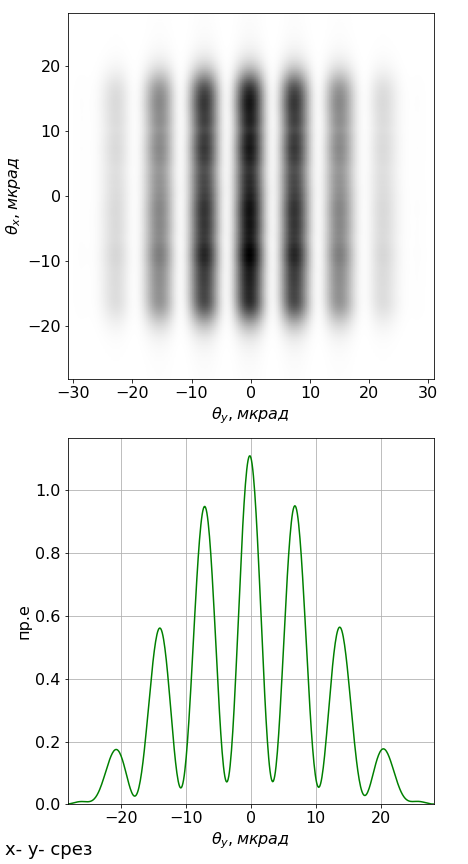
\includegraphics[width=1\linewidth]{y_slits_width_3e-05_separation_7.5e-05_.png}
		\caption{}
		\label{fig:y_slits_75}
	\end{subfigure}
	\begin{subfigure}{0.33\textwidth}
		\centering
		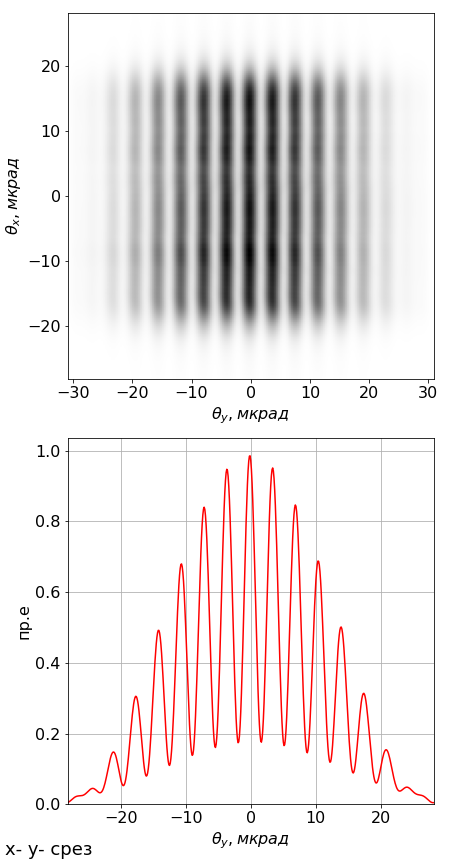
\includegraphics[width=1\linewidth]{y_slits_width_3e-05_separation_0.00015_.png}
		\caption{}
		\label{fig:y_slits_150}
	\end{subfigure}\hfill
	\begin{subfigure}{0.33\textwidth}
		\centering
		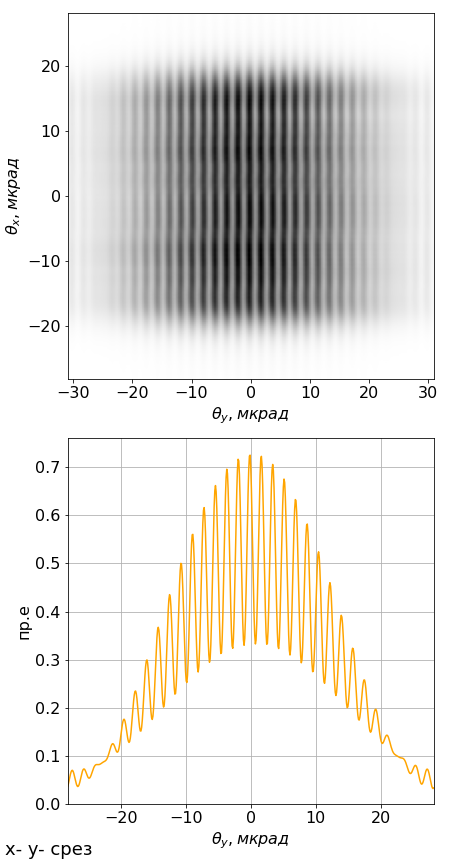
\includegraphics[width=1\linewidth]{y_slits_width_3e-05_separation_0.0003_.png}
		\caption{}
		\label{fig:y_slits_300}
	\end{subfigure}
	\caption{Дифракционные картины для \textit{горизонтального} расположения щелей в дальней зоне, слева на право межщелевой зазор: $75$ мкм, $150$ мкм, $300$ мкм. Цвета линий соответствуют цветам на Рис.~\ref{fig:double_slit_size_corr}}
	\label{fig:y_slits}
\end{figure}
\noindent В этом направлении излучение обладает большей степенью когерентности.

\section{Отражение от неидеального зеркала}\label{section:roughness}
CЕРВАЛ применим для расчёта отражения частично когерентного излучения от зеркал с шероховатостями. При отражении от неидеального зеркала волновой фронт деформируется, что может в значительной степени влиять на размер и максимальную интенсивность излучения в фокусе, а также на когерентные свойства излучения. Ошибки по высоте $\delta h$ профиля зеркала вносят фазовый сдвиг: 
\begin{align}
	\phi = \cfrac{4 \pi \delta h}{\lambda} \sin{(\theta_i)},
	\label{eq:roughness}
\end{align}
где $\theta_i$ -- угол падения, отсчитываемый от поверхности зеркала. 

Формула~\ref{eq:roughness} даёт простой путь учёта шероховатости поверхностей при моделировании в волновом подходе. Таким образом, действие неидеальной поверхности учитывается как фазовый фактор, модулирующий волновой фронт. Альтернативный подход -- использование пошагового моделирования процесса отражения волнового фронта от поверхности зеркала с учётом прохождения излучения в вещество, так называемый (англ.) split-step method. Сравнительный анализ этих двух подходов приведён в работе~\cite{serkez_design_2015}, где показано совпадение оценки числа Штреля для различных величин шероховатостей. Вопросы моделирования профиля зеркала $\delta h$ рассматриваются в Приложении~\ref{AppendixB}.

Для моделирования была выбрана та же оптическая схема, что и для фокусировки с апертурой в разделе~\ref{section:focusing_system_with_aperture}. В данном примере, в качестве фокусирующих элементов, рассматриваются зеркала с тем же фокусным расстоянием -- 12,5 метра. Апертура была исключена из рассмотрения, чтобы показать действие неидеального зеркала на свойства излучения при отражении. 

На Рис.~\ref{fig:x_SERVAL_radiaiton_after_reflection_2d_3A} и~\ref{fig:y_SERVAL_radiaiton_after_reflection_2d_3A} представлены распределения излучения после отражения от неидеальных фокусирующих зеркал в \textit{двух случаях}: вертикального расположения зеркала (Рис.~\ref{fig:x_SERVAL_radiaiton_after_reflection_2d_3A}) и горизонтального (Рис.~\ref{fig:y_SERVAL_radiaiton_after_reflection_2d_3A}). Среднеквадратичная амплитуда шероховатостей зеркала $h_{rms}$ в каждом случае составляет $0,3$ нм. Распределение излучения представлено после отражения и распространения волнового фронта на $12,5$ м через пустое пространство.
\begin{figure}[H]
	\centering
	\begin{subfigure}{0.49\textwidth}
		\centering
		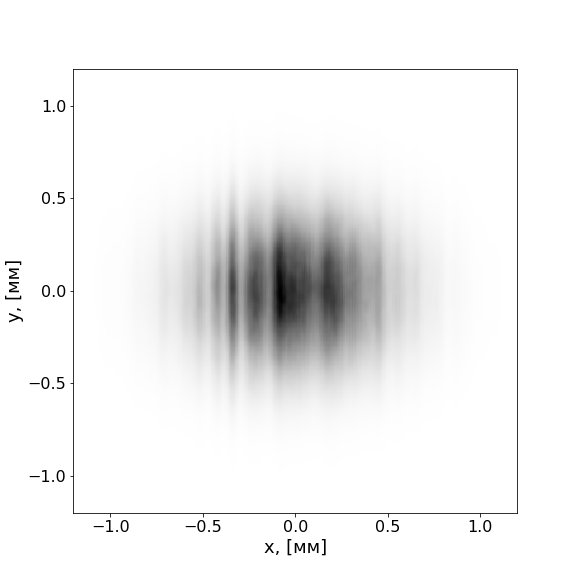
\includegraphics[width=1\linewidth]{x_SERVAL_radiaiton_after_reflection_2d_3.0_A.png}
		\caption{}
		\label{fig:x_SERVAL_radiaiton_after_reflection_2d_3A}
	\end{subfigure}
	\begin{subfigure}{0.49\textwidth}
		\centering
		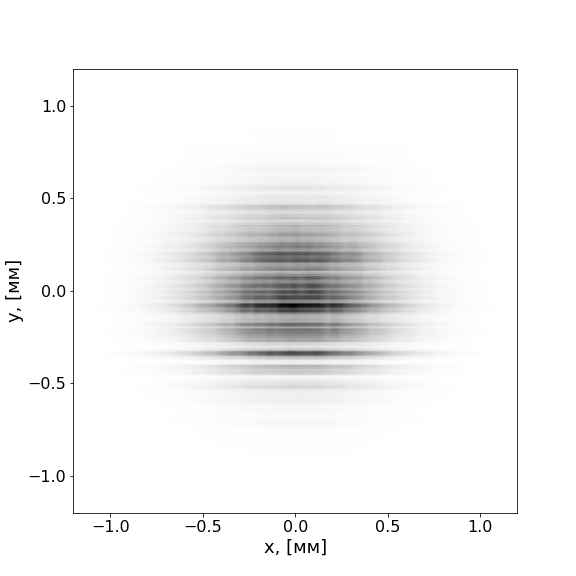
\includegraphics[width=1\linewidth]{y_SERVAL_radiaiton_after_reflection_2d_3.0_A.png}
		\caption{}
%{Распределение интенсивности излучения после отражения и $12,5$ м пустого пространства, ошибки по высоте введены по вертикальному направлению}
		\label{fig:y_SERVAL_radiaiton_after_reflection_2d_3A}
	\end{subfigure}
	\caption{Распределение интенсивности излучения после отражения от неидеального фокусирующего зеркал и распространение через $12,5$ м пустого пространства. На Рис.~\ref{fig:x_SERVAL_radiaiton_after_reflection_2d_3A} зеркало ориентировано \textit{вертикально}, на Рис.~\ref{fig:y_SERVAL_radiaiton_after_reflection_2d_3A} зеркало ориентировано \textit{горизонтально}.}
	\label{fig:SERVAL_radiaiton_after_reflection_2d_3A}
\end{figure}
\noindent Видно, при вертикальной ориентации зеркала модуляции волнового фронта более сглажены из-за меньшей степени когерентности в горизонтальном направлении, в отличии горизонтального расположения зеркала -- направление с большей степенью когерентности.

Для сравнения того, как влияют разные профили зеркала на свойства излучения после пропагации и в фокусе, на Рис.~\ref{fig:x_SERVAL_radiaiton_after_reflection}-\ref{fig:y_SERVAL_radiaiton_in_focus} представлены соответствующие распределения интенсивности излучения после отражения от зеркала со среднеквадратичными амплитудами шероховатостей равными $0,3$ нм и $0,6$ нм. Сравнение приведено для \textit{двух ориентаций} моделируемого зеркала: зеркало ориентировано вертикально Рис.~\ref{fig:x_SERVAL_radiaiton_after_reflection},~\ref{fig:x_SERVAL_radiaiton_in_focus}. и, соответственно, горизонтально на Рис.~\ref{fig:y_SERVAL_radiaiton_after_reflection},~\ref{fig:y_SERVAL_radiaiton_in_focus}. Для всех случаев была выбрана $PSD$ функция с коэффициентом $\beta = -1,8$, нормированная на соответствующие значения среднеквадратического отклонения ошибок профиля. Характер $PSD$ функции профилей рентгеновских зеркал разобран в Приложении~\ref{AppendixB}.

\begin{figure}[H] 
	\centering 	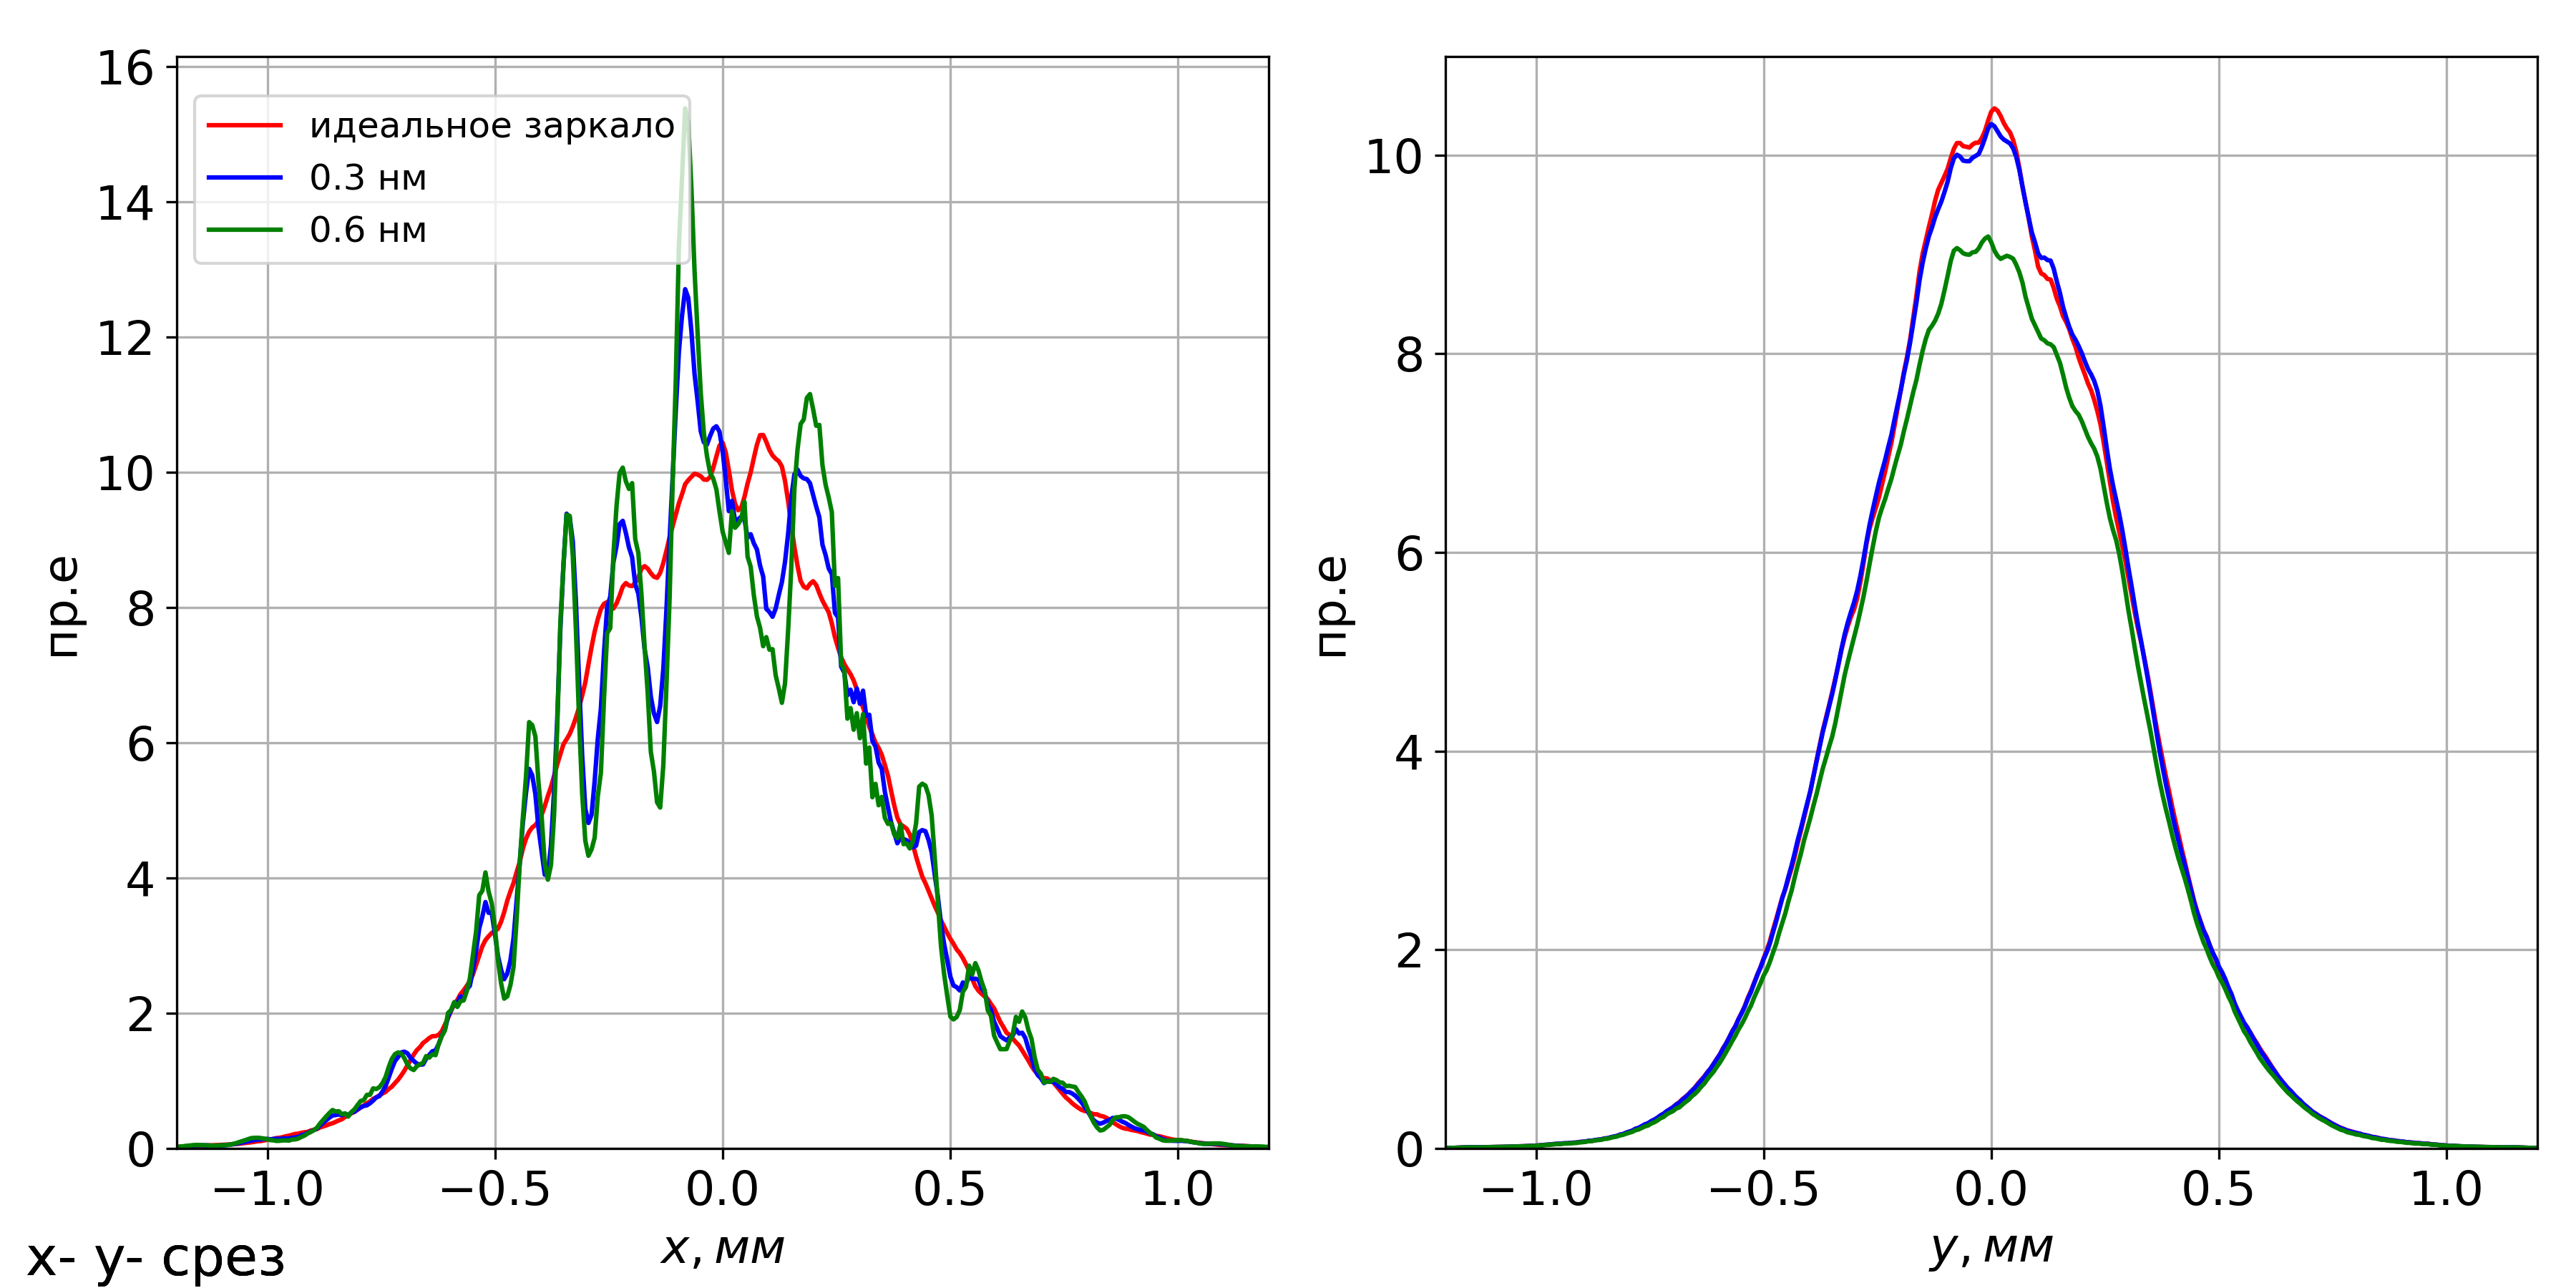
\includegraphics[width=0.99\linewidth]{x_SERVAL_radiaiton_after_reflection.png}
	\caption{Распределение интенсивности излучения после пропагции на 12,5 м от зеркала, зеркало ориентировано \textit{вертикально}}
	\label{fig:x_SERVAL_radiaiton_after_reflection}
\end{figure}

\begin{figure}[H] 
	\centering 	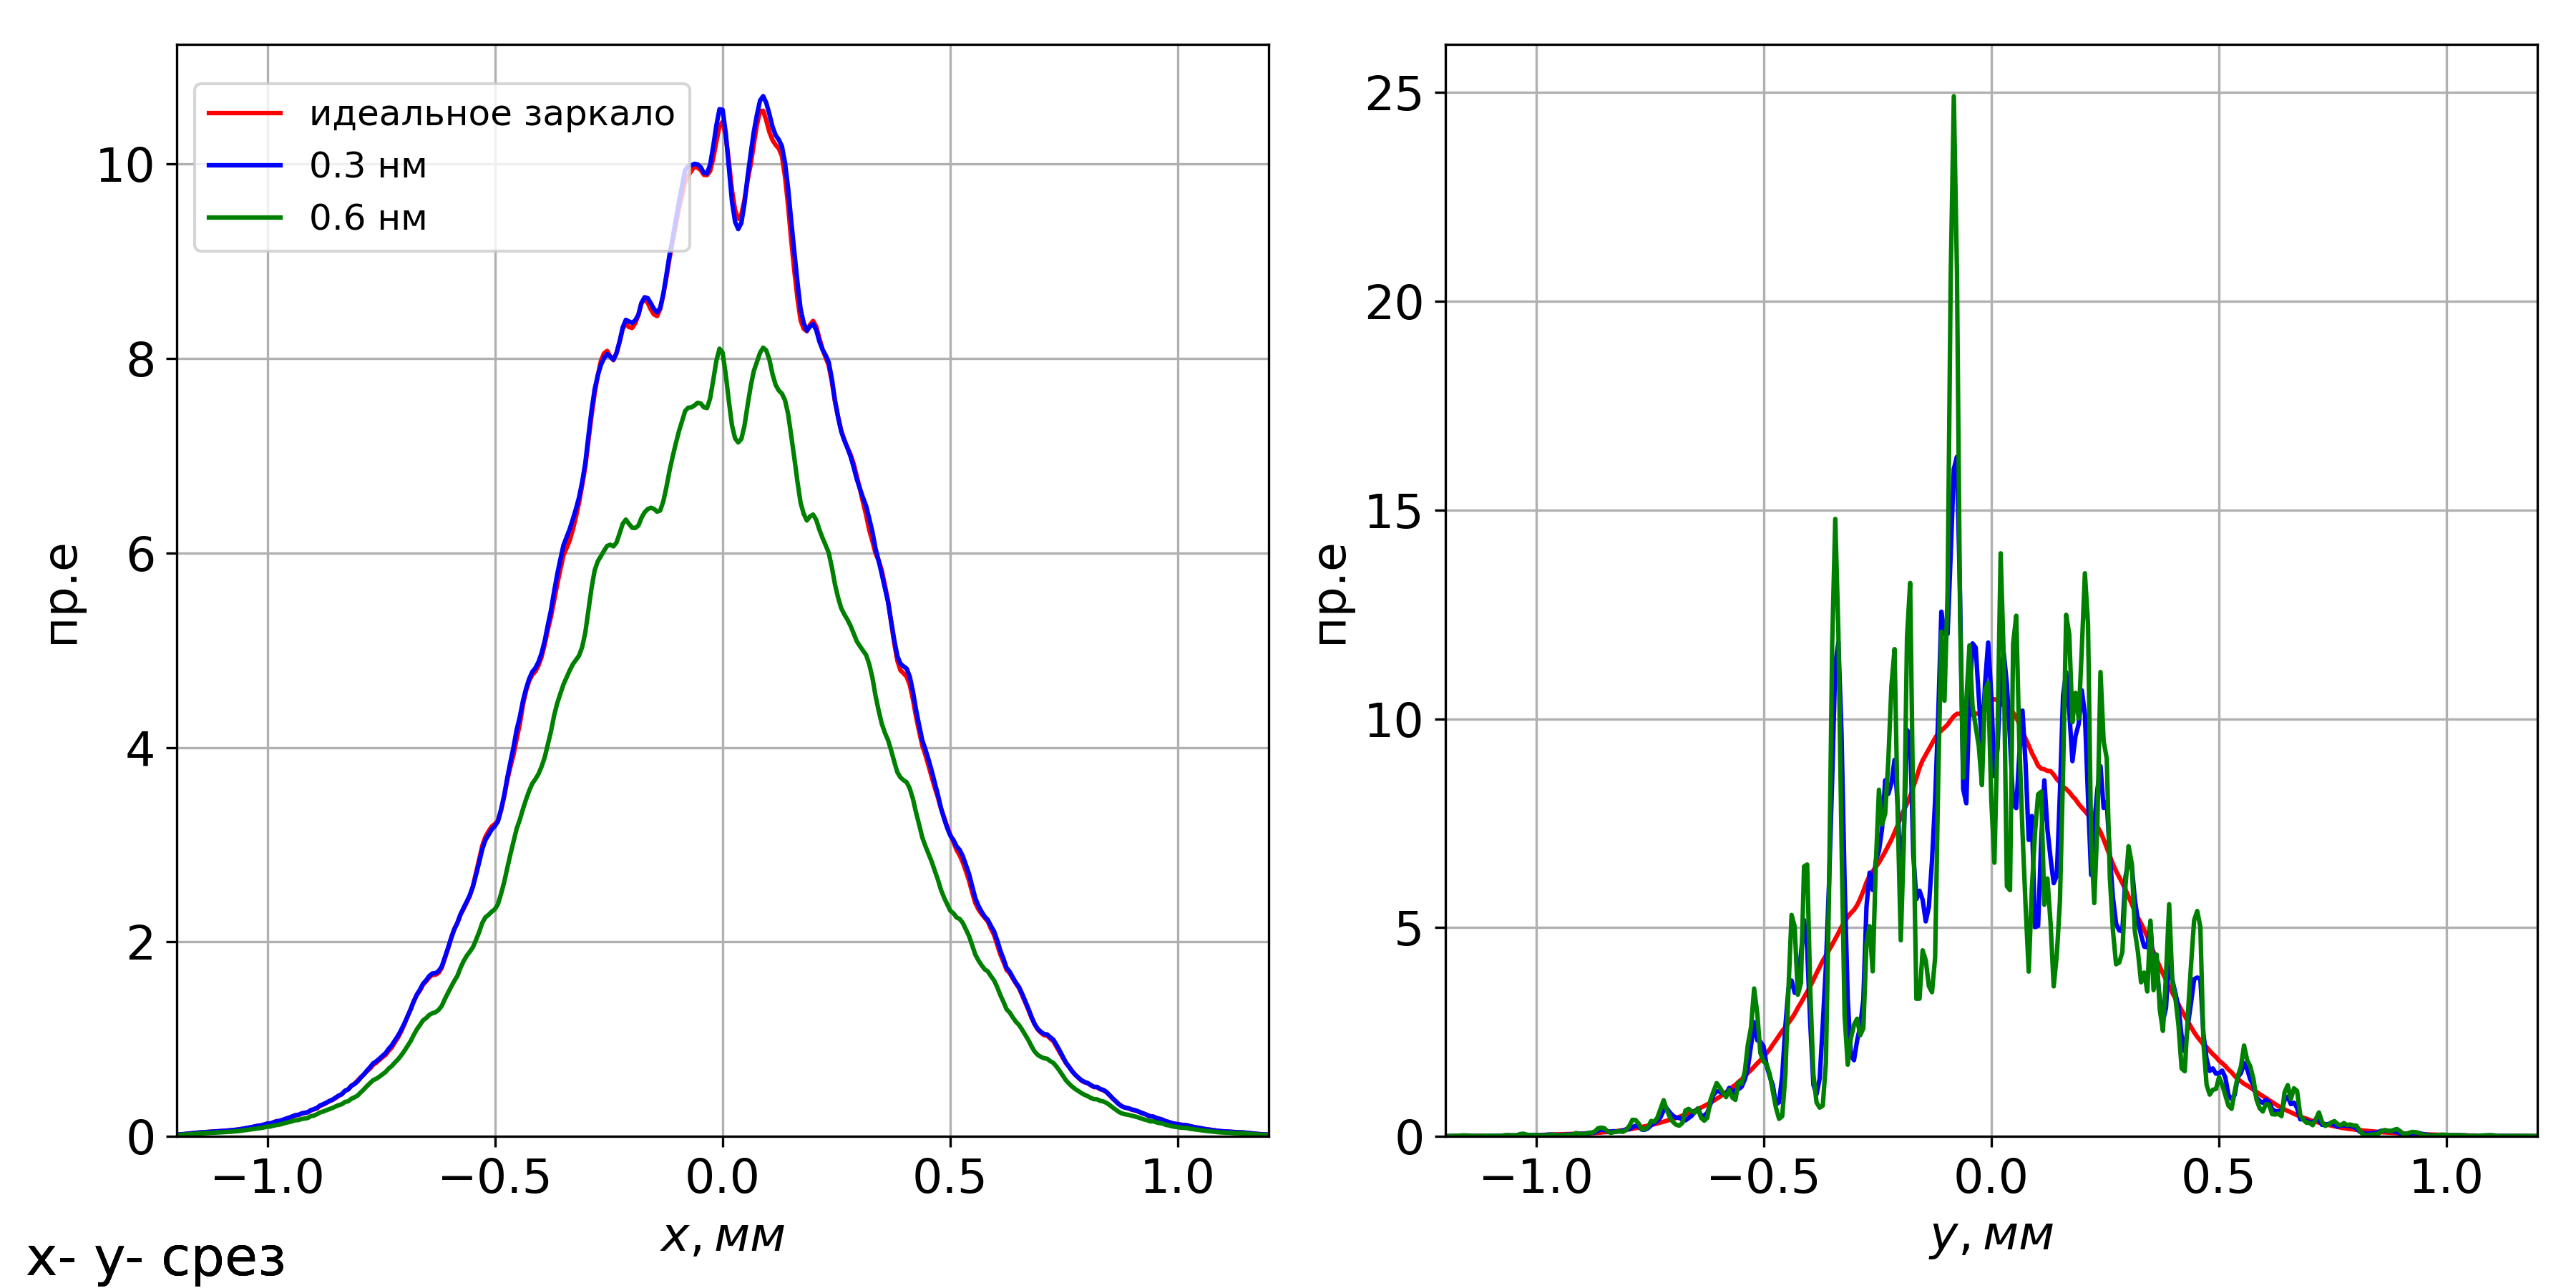
\includegraphics[width=0.99\linewidth]{y_SERVAL_radiaiton_after_reflection.png}
	\caption{Распределение интенсивности излучения после распространение на 12,5 м от зеркала, зеркало ориентировано \textit{горизонтально}}
	\label{fig:y_SERVAL_radiaiton_after_reflection}
\end{figure}
\noindent При генерации профиля зеркала выбиралось одинаковое начальное число (англ. seed) для генерации псевдослучайной величины, что необходимо для статистической воспроизводимости результатов. Именно поэтому модуляции распределений на Рис.~\ref{fig:x_SERVAL_radiaiton_after_reflection} и~\ref{fig:y_SERVAL_radiaiton_after_reflection} при увеличении величины шероховатости просто повторяют свою форму, но с большей амплитудой.

На Рис.~\ref{fig:x_SERVAL_radiaiton_in_focus} и~\ref{fig:y_SERVAL_radiaiton_in_focus} представлены распределения интенсивности излучения на образце (в фокусе).
\begin{figure}[H] 
	\centering 	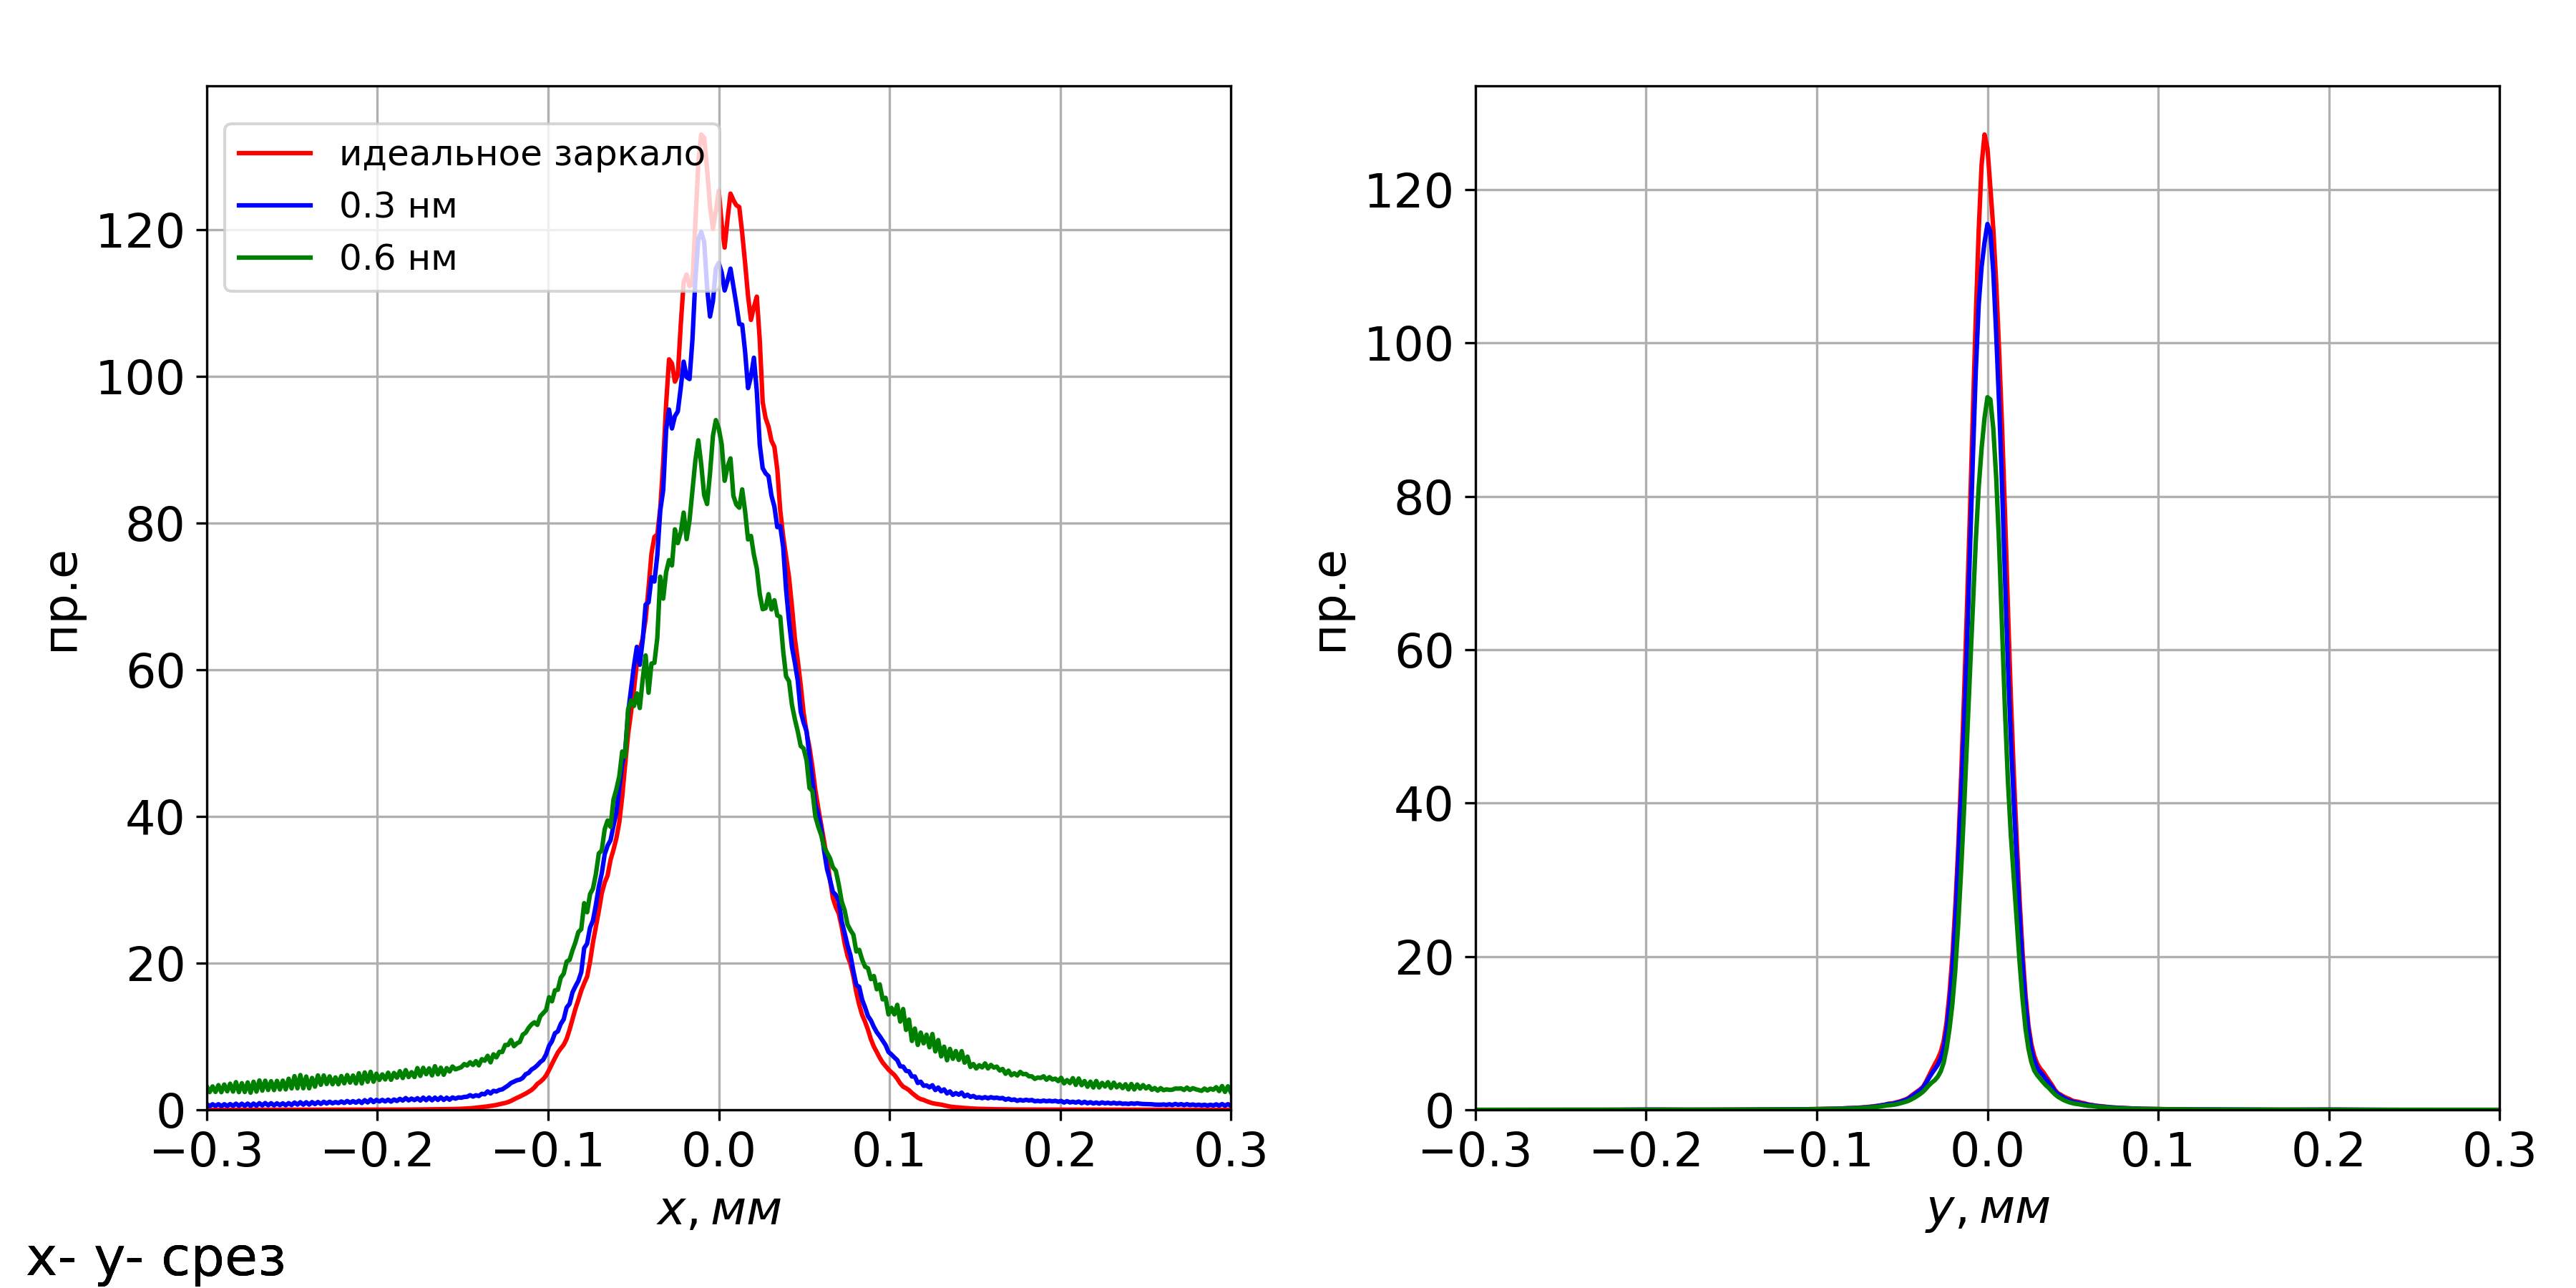
\includegraphics[width=0.99\linewidth]{x_SERVAL_radiaiton_in_focus.png}
	\caption{Распределение интенсивности излучения в фокусе, зеркало в данном случае ориентировано \textit{вертикально}}
	\label{fig:x_SERVAL_radiaiton_in_focus}
\end{figure}

\begin{figure}[H] 
	\centering 	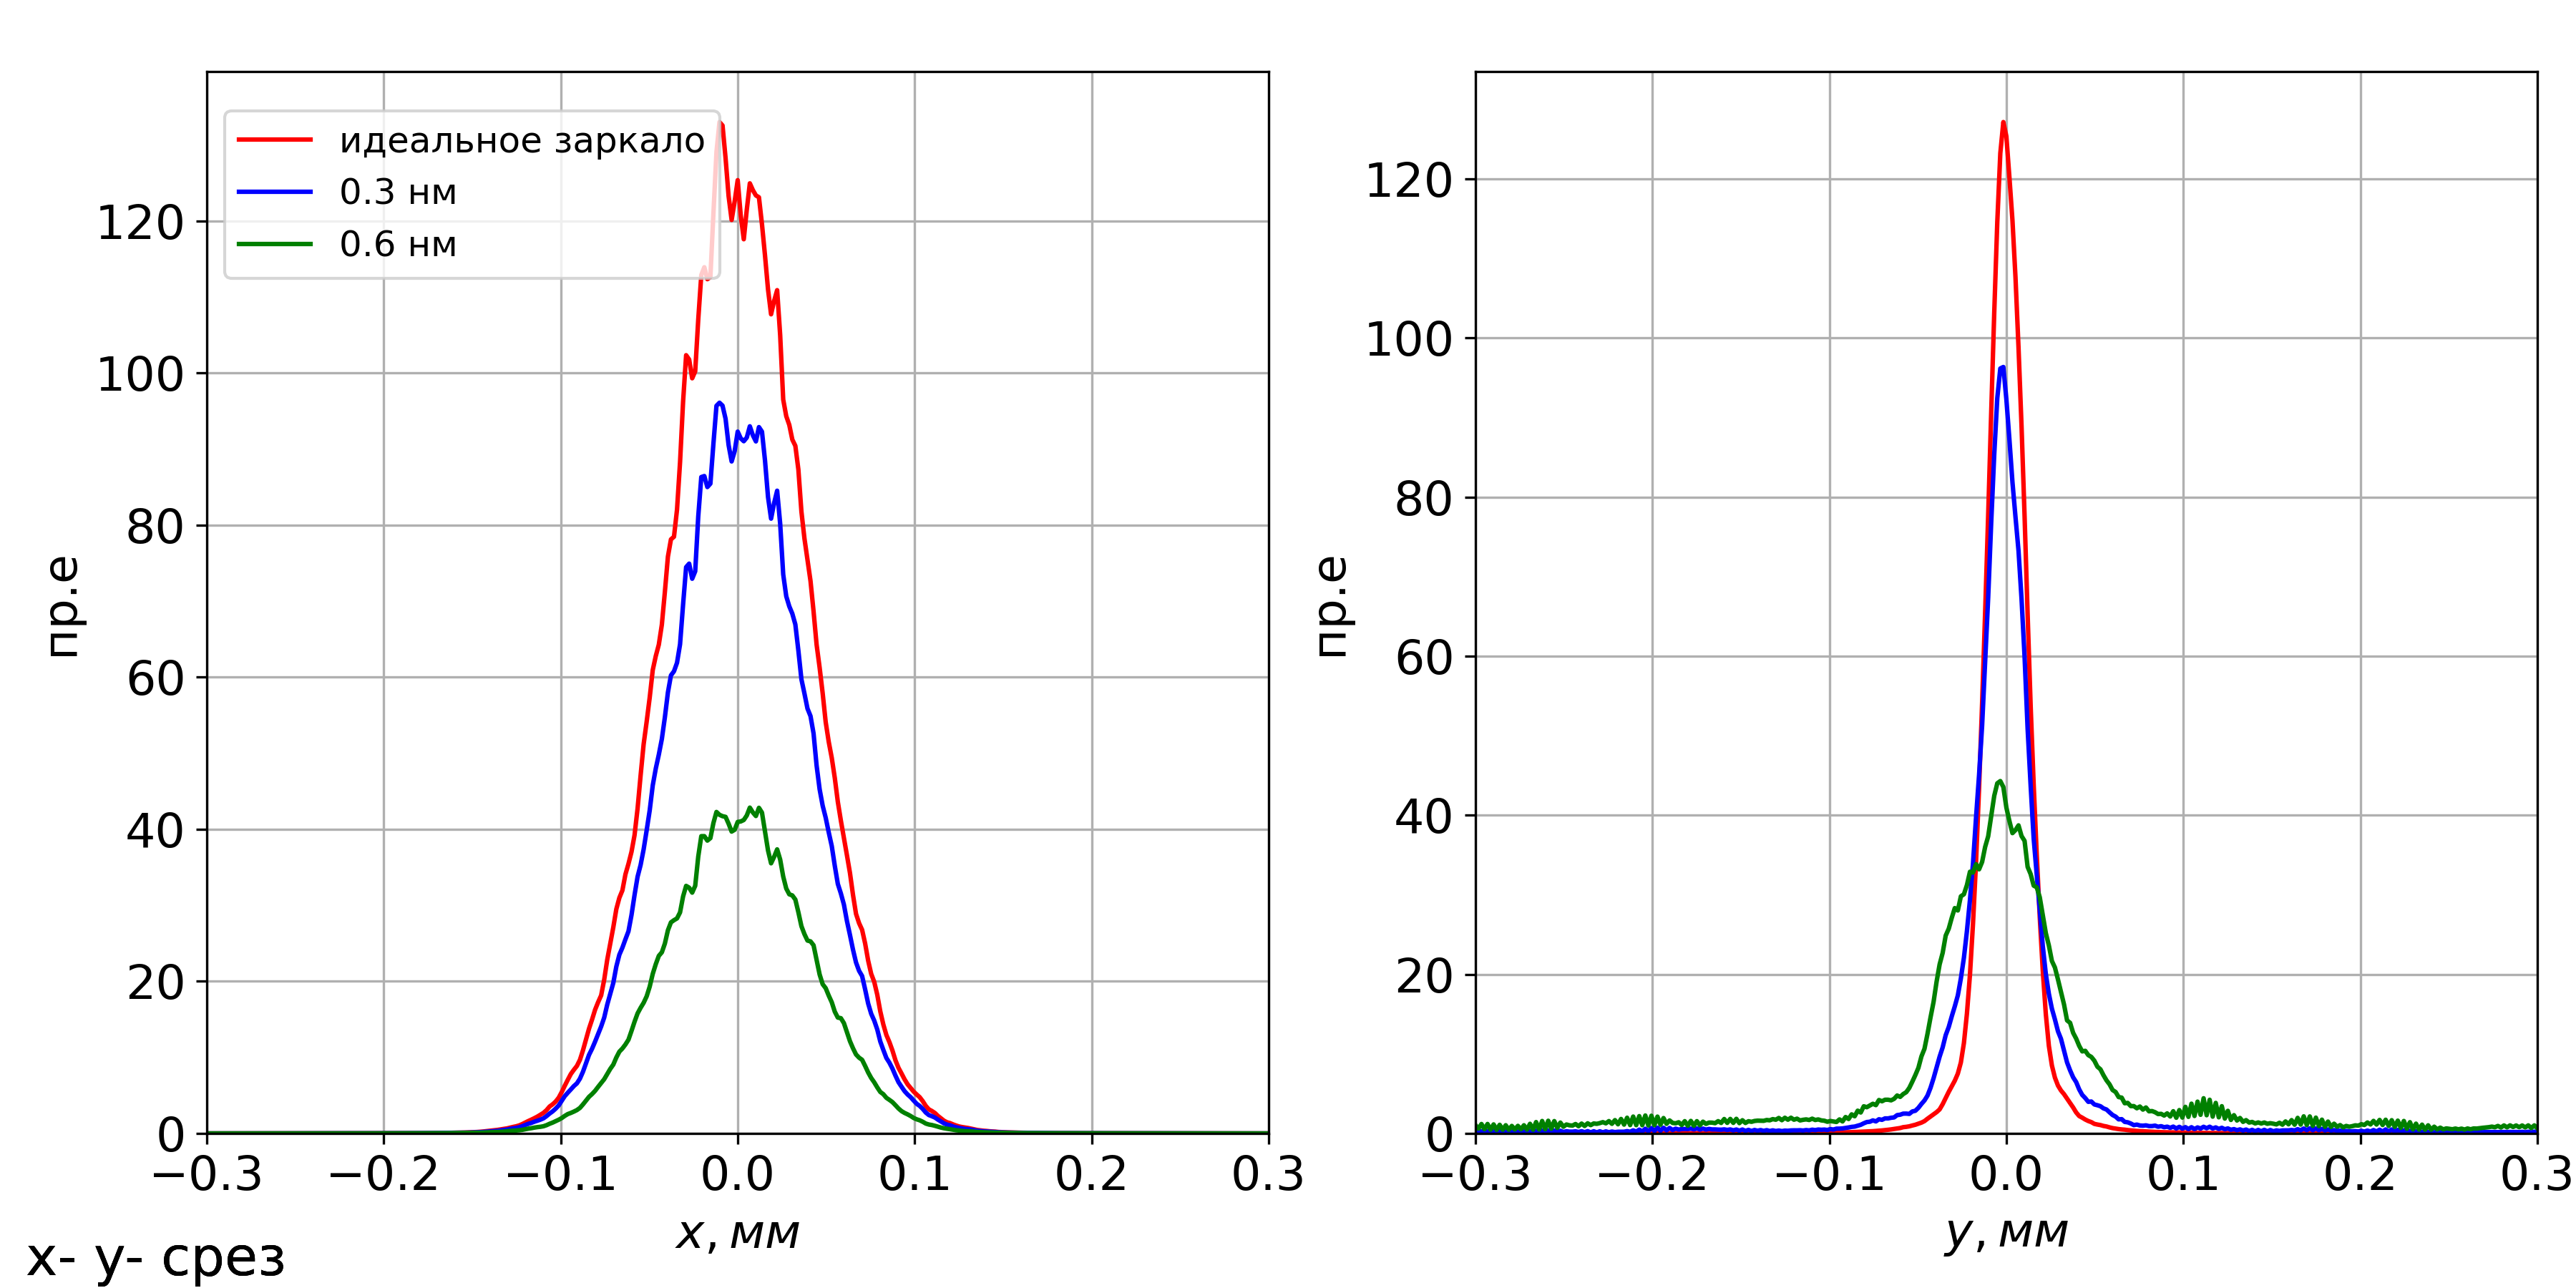
\includegraphics[width=0.99\linewidth]{y_SERVAL_radiaiton_in_focus.png}
	\caption{Распределение интенсивности излучения в фокусе, зеркало ориентировано \textit{горизонтально}}
	\label{fig:y_SERVAL_radiaiton_in_focus}
\end{figure}

Как видно на Рис.~\ref{fig:x_SERVAL_radiaiton_in_focus} и~\ref{fig:y_SERVAL_radiaiton_in_focus} шероховатости приводят к расплыванию фокусного пятна и, следственно, падению пиковой амплитуды интенсивности поля. Этот эффект играет критическую роль, например, для монохроматоров, основанных на дифракционных решётках, где размер фокусного пятна определяет разрешающую способность монохроматора. Поэтому следует налагать довольно жёсткие требования на среднеквадратичные амплитуды шероховатостей рентгеновских зеркал,~\cite{strocov_high-resolution_2010},~\cite{sankari_hippie_nodate}. 

